%% ----------------------------------------------------------------
%% Thesis.tex -- MAIN FILE (the one that you compile with LaTeX)
%% ---------------------------------------------------------------- 

% Set up the document
\documentclass[a4paper, 11pt, oneside]{Thesis}  % Use the "Thesis" style, based on the ECS Thesis style by Steve Gunn
\graphicspath{{Figures/}}  % Location of the graphics files (set up for graphics to be in PDF format)

% Include any extra LaTeX packages required
\usepackage[square, numbers, comma, sort&compress]{natbib}  % Use the "Natbib" style for the references in the Bibliography
\usepackage{verbatim}  % Needed for the "comment" environment to make LaTeX comments
\usepackage{vector}  % Allows "\bvec{}" and "\buvec{}" for "blackboard" style bold vectors in maths
\usepackage{wrapfig}
\hypersetup{urlcolor=blue, colorlinks=true}  % Colours hyperlinks in blue, but this can be distracting if there are many links.

%% ----------------------------------------------------------------
\begin{document}
\frontmatter	  % Begin Roman style (i, ii, iii, iv...) page numbering

% Set up the Title Page
\title  {Thesis}
\authors  {\texorpdfstring
            {\href{your web site or email address}{Junjie Zhang}}
            {Junjie Zhang}
            }
\addresses  {\groupname\\\deptname\\\univname}  % Do not change this here, instead these must be set in the "Thesis.cls" file, please look through it instead
\date       {\today}
\subject    {}
\keywords   {}

\maketitle
%% ----------------------------------------------------------------

\setstretch{1.3}  % It is better to have smaller font and larger line spacing than the other way round

% Define the page headers using the FancyHdr package and set up for one-sided printing
\fancyhead{}  % Clears all page headers and footers
\rhead{\thepage}  % Sets the right side header to show the page number
\lhead{}  % Clears the left side page header

\pagestyle{fancy}  % Finally, use the "fancy" page style to implement the FancyHdr headers

%% ----------------------------------------------------------------
% Declaration Page required for the Thesis, your institution may give you a different text to place here
\Declaration{

\addtocontents{toc}{\vspace{1em}}  % Add a gap in the Contents, for aesthetics

I, Junjie Zhang, declare that this thesis titled, `Weather Classification' and the work presented in it are my own. I confirm that:

\begin{itemize} 
\item[\tiny{$\blacksquare$}] This work was done wholly or mainly while in candidature for a research degree at this University.
 
\item[\tiny{$\blacksquare$}] Where any part of this thesis has previously been submitted for a degree or any other qualification at this University or any other institution, this has been clearly stated.
 
\item[\tiny{$\blacksquare$}] Where I have consulted the published work of others, this is always clearly attributed.
 
\item[\tiny{$\blacksquare$}] Where I have quoted from the work of others, the source is always given. With the exception of such quotations, this thesis is entirely my own work.
 
\item[\tiny{$\blacksquare$}] I have acknowledged all main sources of help.
 
\item[\tiny{$\blacksquare$}] Where the thesis is based on work done by myself jointly with others, I have made clear exactly what was done by others and what I have contributed myself.
\\
\end{itemize}
 
 
Signed:\\
\rule[1em]{25em}{0.5pt}  % This prints a line for the signature
 
Date:\\
\rule[1em]{25em}{0.5pt}  % This prints a line to write the date
}
\clearpage  % Declaration ended, now start a new page

% The Abstract Page
% \addtotoc{Abstract}  % Add the "Abstract" page entry to the Contents

\begin{abstract}
   Weather classification is an important field in computer vision. For similar weather condition, there are some obstacles for extracting features from outdoor images. In this paper, we present a novel approach to classify cloudy and sunny weather. Inspired by recent study of deep multi-layer neural network and spatial pyramid polling, generate a model based on imagenet dataset. Starting with parameters trained from more than 1 million images, we fine-tune the parameters. Experiment demonstrates that our classifier can achieve the state of the art accuracy.
\end{abstract}



\clearpage  % Abstract ended, start a new page
%% ----------------------------------------------------------------

\setstretch{1.3}  % Reset the line-spacing to 1.3 for body text (if it has changed)

% The Acknowledgements page, for thanking everyone
\acknowledgements{
\addtocontents{toc}{\vspace{1em}}  % Add a gap in the Contents, for aesthetics

The acknowledgements and the people to thank go here, don't forget to include your project advisor\ldots

}
\clearpage  % End of the Acknowledgements
%% ----------------------------------------------------------------

\pagestyle{fancy}  %The page style headers have been "empty" all this time, now use the "fancy" headers as defined before to bring them back


%% ----------------------------------------------------------------
\lhead{\emph{Contents}}  % Set the left side page header to "Contents"
\tableofcontents  % Write out the Table of Contents

%% ----------------------------------------------------------------
\lhead{\emph{List of Figures}}  % Set the left side page header to "List if Figures"
\listoffigures  % Write out the List of Figures

%% ----------------------------------------------------------------
\lhead{\emph{List of Tables}}  % Set the left side page header to "List of Tables"
\listoftables  % Write out the List of Tables

%% ----------------------------------------------------------------
\setstretch{1.5}  % Set the line spacing to 1.5, this makes the following tables easier to read
\clearpage  % Start a new page
\lhead{\emph{Abbreviations}}  % Set the left side page header to "Abbreviations"
\listofsymbols{ll}  % Include a list of Abbreviations (a table of two columns)
{
% \textbf{Acronym} & \textbf{W}hat (it) \textbf{S}tands \textbf{F}or \\
\textbf{LAH} & \textbf{L}ist \textbf{A}bbreviations \textbf{H}ere \\

}

%% ----------------------------------------------------------------
\clearpage  % Start a new page
\lhead{\emph{Physical Constants}}  % Set the left side page header to "Physical Constants"
\listofconstants{lrcl}  % Include a list of Physical Constants (a four column table)
{
% Constant Name & Symbol & = & Constant Value (with units) \\
Speed of Light & $c$ & $=$ & $2.997\ 924\ 58\times10^{8}\ \mbox{ms}^{-\mbox{s}}$ (exact)\\

}

%% ----------------------------------------------------------------
\clearpage  %Start a new page
\lhead{\emph{Symbols}}  % Set the left side page header to "Symbols"
\listofnomenclature{lll}  % Include a list of Symbols (a three column table)
{
% symbol & name & unit \\
$c$ & distance & m \\
$P$ & power & W (Js$^{-1}$) \\
& & \\ % Gap to separate the Roman symbols from the Greek
$\omega$ & angular frequency & rads$^{-1}$ \\
}
%% ----------------------------------------------------------------
% End of the pre-able, contents and lists of things
% Begin the Dedication page

\setstretch{1.3}  % Return the line spacing back to 1.3

\pagestyle{empty}  % Page style needs to be empty for this page
\dedicatory{For/Dedicated to/To my\ldots}

\addtocontents{toc}{\vspace{2em}}  % Add a gap in the Contents, for aesthetics


%% ----------------------------------------------------------------
\mainmatter	  % Begin normal, numeric (1,2,3...) page numbering
\pagestyle{fancy}  % Return the page headers back to the "fancy" style

% Include the chapters of the thesis, as separate files
% Just uncomment the lines as you write the chapters
% Chapter 1
\title  {Weather Classification}
\chapter{Introduction} % Write in your own chapter title
\label{Chapter1}
\lhead{Chapter 1. \emph{Introduction}} % Write in your own chapter title to set the page header


\section{Overview}

Computer is one of the most significant inventions in history. It provides huge power in data processing field, like scientific computation. Also, computer system can aid human being in daily life, for example driverless vehicles. However, human brain still has compelling advantage in some fields, like identifying our keys in our pocket by feel. The complex processes of taking in raw data and taking action based on the pattern are regarded as pattern recognition. Pattern recognition has been important for people daily life for a long period and human brain has developed an advanced neural and cognitive system for such tasks.

Weather classification is one of the most important pattern recognition tasks which relates our work and lives. There are several major kinds of weather conditions, like sunny, cloudy, rainy. And people can classify them easily through eyes. However, it is not a easy job for machines, especially in computer vision literacy. 

In this thesis, I describe an approach to this problem of weather classification based upon the new big trend in machine learning, and more precisely, deep learning. It differs with feature detectors method that extracts features manually and training a model to do classification.  

Compared to shadow learning which includes decision trees, SVM and naive bayes, deep learning passes input data through several non-linearities functions to generate features and does classification based on the features. It generates a mapping and finds a optimist solution.

\section{Statistical Pattern Recognization}

In the statistical approach, the pattern is represented in terms of d dimensional feature vector and each element of the vector describes some subjects of the example. In brief, three components are essential to do statistical pattern recognization. First is a representation of the model. Second is an objective function used to evaluating the accuracy of the model. Third is an optimization method for learning a model with minimum errors.

\section{Artificial Neural Networks}

Artificial neural networks(ANNs) were proposed in the mid-20th century. The term is inspired by the structure of neural networks in the brain. It is one of the most successful statistical learning models used to approximate functions. Learning with ANNs yields an effective learning paradigm and has achieved cutting-edge performance in computer vision. 

The single-layer perceptron  has shown great success for a simple model. For increasing complex models and applications, multi-layer perceptron has exhibited the power of features learning. With hardware developing At the same time, the demanding of more efficient optimizing and model evoluation methods is needed for BIG DATA. 

Recent development in ANNs approaches have giantly advanced the performance of state-of-the-art visual recognition systems. With implementing deep convolutional neural networks, it achieves top accuracy in ImageNet Challenge. The model has been used in related fields and succeeds in competition.

\section{Weather Classification}

Weather classification is an important job in daily life. In this thesis, we are focused on two class weather conditions, sunny and cloudy. 

There are some obstacles in front of weather classification. First, because inputting pixels are independent and high dimension, say a 500x500 RPG image means 750000 pixels, computation is huge. Second, some simple middle level image characters are difficult to machines, like light, shading, sun shine. It is still not easy to detect these characters with high accuracy.  Thirdly, there are no decisive features, for example brightness and lightness, to classify scene. For example, sun shine can be both found in sunny and cloudy weather. Last but not least, outdoor images are various background.


 % Introduction

% Chapter 2

\chapter{Background} % Write in your own chapter title
\label{Chapter2}
\lhead{Chapter 2. \emph{Background and Related Work}}


\section{Single-Layer Networks}

Artificial neurons were introduced as information processing devices more than fifty years ago\citep{mcculloch1943logical}. Following the early work, perceptrons were deployed in layers to do pattern recognition job. A lot of resource was invested in researching capability of learning perceptrons theoretically and experimentally. As shown in Figure 2.1, a perceptron computes a weighted summation of its n inputs and then thresholds the result to give a binary output y. We can treat n input as an vector with n elements, and represent the vector as either class A(for output +1) or class B(for output -1).
\graphicspath{ {./Figures/} }
\begin{figure}[!htb]
\centering
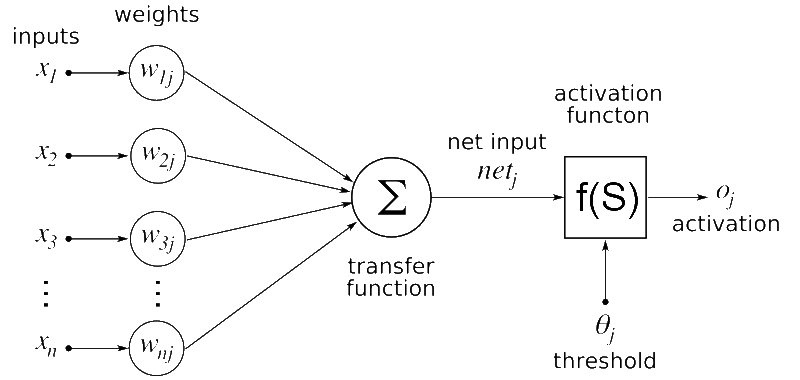
\includegraphics[width=0.8\textwidth]{Figure2-1.png}
\caption{\label{fig:perceptron}Diagram of a perceptron.}
\end{figure}


Each output is updated according to the equation:
\begin{equation}\label{eq:BasicEq}
y_{i} = f(h_{i}) = f\left(\sum_{j}w_{ij}x_{j}\right)
\end{equation}
where $y_{i}$ is the $i$th output, $h_{i}$ is the net input into node $i$, The weight $w_{ij}$ connects the $i$th output and the $j$th input, and $x_{j}$ is the $j$th input. The function $f(h)$ is the activation function and usually makes up the form
\begin{equation}\label{eq:FullEq}
f(h) = sign(h) = 
  \begin{cases}
    -1       & \quad h < 0 \\
    1  & \quad h \geq 0\\
  \end{cases}
\end{equation}
We can also represent \ref{eq:FullEq} in vector notation, as in 
\begin{equation}\label{eq:UsedEq}
y = f(h) = f(\bf w \cdot x)
\end{equation}
where \textbf{w} and \textbf{x} can be regarded as $nx1$ dimensional column vectors, and $n$ is the number of input data.
The term $w \cdot x$ in \ref{eq:UsedEq} constructs a $(n-1)$-dimension hyperplane which passes the origin. The hyperplane can be shifted by adding an parameter to \ref{eq:BasicEq}, for example
\begin{equation}\label{eq:WithBias}
y = f(h) = f(\bf w \cdot x + b)
\end{equation}
We can have the same effect by putting a constant value $1$ and increase the size of $x$ and $w$ by one. The extra weight $w$ with fixed value 1 is called \textit{bias weight}; it is adaptive like other weights and provides flexibility to hyperplane. Then we get:
\begin{equation}\label{eq:finalEq}
y = f(h) = f(\sum_{i=0}^{n}w_{i}x_{i})
\end{equation}
The aim of learning is to find a set of weights $w_{i}$ so that:
\begin{align*}
y = f(\sum_{i=0}^{n}w_{i}x_{i}) = 1  & \quad x \in Class A\\
y = f(\sum_{i=0}^{n}w_{i}x_{i}) = 0  & \quad x \in Class B
\end{align*}


\section{Multi-Layer Networks}

Single-layer networks have some important limitation in terms of the representing range of functions. We are seeking to learn the nonlinearity as the linear discriminant.To improve the representation capability, we can stack layers networks. This is the approach of multilayer neural networks. Multilayer neural networks implement linear discriminants via mapping input data to a nonlinear space. They can use fairly simple algorithms to learn form of the nonlinearity from training data.

In the thesis, we limit multi-layer networks in subset of feedforward networks. As feedforward networks can provide a general mechanism for representing nonlinear functional mapping between a set of input data and a set of labels. The \ref{fig:ffnet} is a feedforward network having two layers of adaptive weights.

\begin{figure}[!htb]
\centering
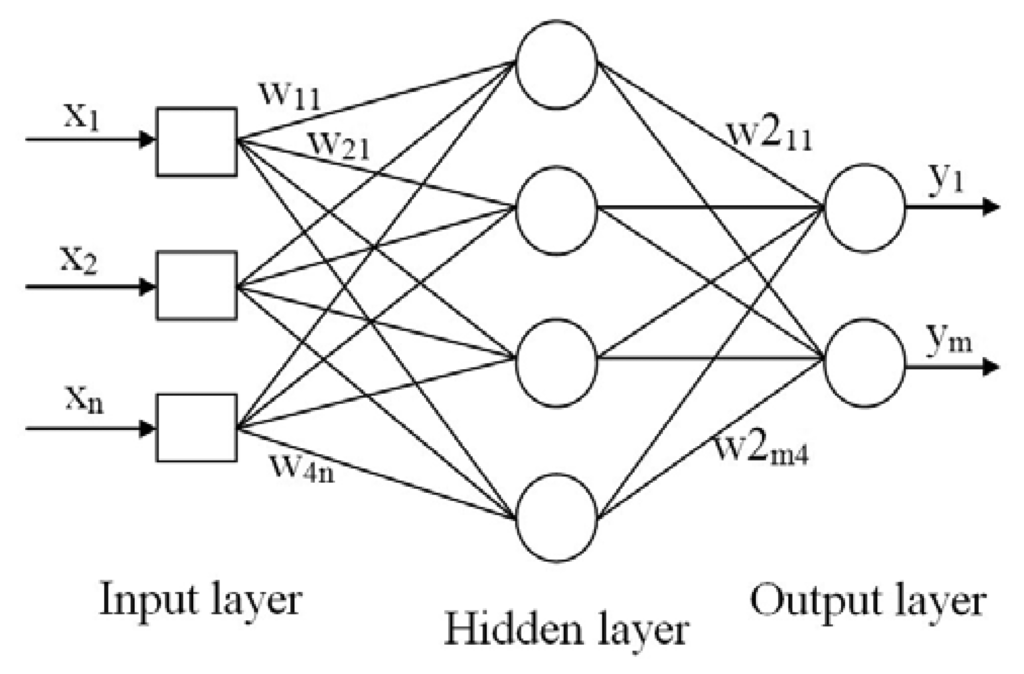
\includegraphics[width=0.8\textwidth]{Figure2-2.png}
\caption{\label{fig:ffnet}Diagram of a feedford neural networks.}
\end{figure}

In the example, the middle column perceptrons act as hidden units. The network has $n$ inputs, $4$ hidden units and $m$ output units. The network diagram represents the function in the form
\begin{equation}\label{eq:ffEq}
y_{m} = \hat{f}\Big(\sum_{j=0}^{m}w_{j4}^{(2)}f\big(\sum_{i=0}^{n}w_{4i}^{(1)}x_{i}\big)\Big)
\end{equation}
In the \ref{eq:ffEq}, outer activation function could be different with the inner one.

There are some choices for activation functions, sigmoid and tanh are related and can provide high capability with continuous input data. Logistic activation function sigmoid can be represented as 
\begin{equation}\label{eq:sigmoid}
f(x) = \frac{1}{1+e^{-x}}
\end{equation}
Its outputs lies in range $(0,1)$. We can do a linear transformation $hat{x}=x/2$ on input data and a linear transformation $hat{y}=2y-1$ on the output. Then we can get an equivalent activation function tanh which can be represented as
\begin{equation}\label{eq:tanh}
f(x) = tanh(x) = \frac{e^{x}-e^{-x}}{e^{x}+e^{-x}}
\end{equation}

The three layer neural network is capable of approximating any function with enough hidden units which means the networks with two layers of weights and sigmoid nonlinearities can provide any accuracy in classification problems. 

\section{Backpropagation}

Multi-layer neural networks can represent mapping from input data to output classes. How to learn a suitable mapping from training dataset? And there is no explicit mapping between output and hidden units. This will be resolved by a popular learning algorithm-backpropagation.

Because networks have differentiable activation functions, the activation of output units can be propagated to hidden units with regard to weights and bias. If we have an error function, we can evaluate derivatives of the error and update the weights to minimize the error function via some optimization methods.

Backpropagation can be applied to find the derivatives of an error function related to the weights and biases in the network via two stages. First, the derivatives of the error functions, for instance sum-of-squares and Jacobian, with respect to the weights must be evaluated. Second, a variety of optimization schemes can be implemented to compute the adjustment of weights based on derivatives. After putting data forward propagation through the network, we can get the output result. It updates weight changes based on grandient descent. Suppose the network has $i$ inputs, $h$ hidden units and $k$ outputs. The update equation can be represented as 
\begin{equation}\label{eq:UpdateWeights}
w(j+1) = w(j) + \Delta w(j)
\end{equation}
where $\Delta w(j)$ defined as 
\begin{equation}\label{eq:DeltaWeights}
\Delta w(j) = -\eta \frac{\partial E}{\partial w}
\end{equation}

For the hidden to output layer weights
\begin{equation}\label{eq:h2oBP}
\Delta w(jk) = -\eta \frac{\partial E}{\partial w_{jk}} = -\eta \delta_{k}y_{j}
\end{equation}
where $$\delta_{k} = \frac{\partial E}{\partial a_{k}} = (y_{k} - t_{k})y_{k}(1 - y_{k})$$

For the hidden layer weights
\begin{equation}\label{eq:hiddenBP}
\Delta w(ij) = -\eta \frac{\partial E}{\partial w_{ij}} = -\eta \delta_{j}y_{i}
\end{equation}
where $$\delta_{j} = \frac{\partial E}{\partial a_{j}} = \displaystyle\sum_{k} \delta_{k}w_{jk}y_{j}(1 - y_{j})$$

The $\delta_{j}$ of a hidden unit is based on the $\delta_{k}$s of output units to which it links. To minimise the error function$E$ with gradient descent, it needs the propagation of errors backwards.

\section{Softmax classifier}

Softmax function, also named normalized exponential, is a generalization of logistic function which squeezes a $d$ dimensional arbitrary real values vector to a $d$ dimensional vector of real values in the range $(0,1)$ that add up to 1. Because the softmax function is the gradient log normalizer of categorical probability distribution, it can be used in probabilistic multiclass classification methods.

The softmax function derives from log linear models and interprets the weights in terms of convenient odds ratios. We can constrain the layer input to the output neurons to be positive and divide by the sum.

The softmax layer begins the same way as normal layer which forms the weighted inputs $z^L_j = \sum_{k} w^L_{jk} x^{L-1}_k + b^L_j$ where $L$ is layer number, $k$ is input data number and $j$ is output neuron number. Then it implements a softmax function to the $z^L_j$ and the activation $a^L_j$ of the $j$ output neuron is
\begin{equation}\label{eq:SoftmaxActivation}
f_j(z) = \frac{e^{z_j}}{\sum_k e^{z_k}}
\end{equation}
The equation \ref{eq:SoftmaxActivation} implies that the output values are all positive and the sum of all values $\sum_k a_k$ is $1$.

Softmax classifier is used to handle a multiclass classification. For a training dataset $(x_{1}, y_{1}), \ldots, (x_{m}, y_{m}), y_{i} \in \{1, 2, \ldots, K\} $ of $m$ labelled examples, label $y$ can have $K$ different values.

Suppose to predict an unseen sample $x$, we will use hypothesis to estimate the probability $P(y=k | x)$ for each value $k = 1, \ldots, K$. For example, we want to compute the probability of the class label on each of $K$ different possible values. Then the neural network will output a $K$ dimensional vectors which represent $K$ estimated probabilities. 
%\begin{equation}\label{eq:SoftmaxPostPro}
\begin{align}
h_{W}(x) =
\begin{bmatrix}
P(y = 1 | x; W) \\
P(y = 2 | x; W) \\
\vdots \\
P(y = K | x; W)
\end{bmatrix}
=
\frac{1}{ \sum_{j=1}^{K}{\exp(W^{(j)\top} x) }}
\begin{bmatrix}
\exp(W^{(1)\top} x ) \\
\exp(W^{(2)\top} x ) \\
\vdots \\
\exp(W^{(K)\top} x ) \\
\end{bmatrix}
\end{align}
%\end{equation}
Where $W^{j}$ are the weights of the model and the normalized distribution ensures that the sum is one.

On the one hand, cross entropy can be used to interpreted softmax classifier. The cross entropy between actual  distribution $p$ and a predicted distribution $q$ is represented as
\begin{equation}\label{eq:CrossEntropyDiff}
H(p,q) = - \sum_x p(x) \log q(x)
\end{equation}
Hence, the task of softmax classifier is to minimize the cross entropy between the actual distribution and the predicted distribution. 

On the other hand, softmax classifier can be interpreted in probability view. Given a sample $(x_i, y_i)$ and parameters $W$, we can compute the normalized probability by
\begin{equation}\label{eq:ProbInter}
P(y_i \mid x_i; W) = \frac{e^{f_{y_i}}}{\sum_j e^{f_j} }
\end{equation}
where $f_{y_i}$ is the score predicted by the model with weights $W$. Therefore the normalized probabilities are computed by exponentiating the values and dividing sum of all values. Then we can minimize the negative log likelihood of the ground truth labels which can be regarded as performing Max Likelihood Estimation(MLE). Instead of MLE, Maximum a posteriori(MAP) can be used to evaluate the performance of the model.

\subsection{Practical issues}

For numerical view, the exponentiation computation is easy overflow. Thus, the output of softmax function is not numeric stable through computing $e^{f_{y_i}}$ and $\sum_j e^{f_{y_j}}$ in straight way. It is important to implement with a normalization trick. It is mathematically equivalent if multiplying a constant $C$ both with top and bottom of the fraction.
\begin{equation}\label{eq:SoftmaxTricks}
\frac{e^{f_{y_i}}}{\sum_j e^{f_j}}
= \frac{Ce^{f_{y_i}}}{C\sum_j e^{f_j}}
= \frac{e^{f_{y_i} + \log C}}{\sum_j e^{f_j + \log C}}
\end{equation}
where $C$ can be any positive value. The $C$ does not change the output value, while it can improve the numerical stability of the computation. An experienced choice of $C$ is to set $\log C = -\max_j f_j$, and it can shift the vector $f$ to preserve the highest value as $0$.

\subsection{Error function}
The error function is used to evaluate the performance of the model. We will generate an error function for softmax regression. An indicator function, $I\{\cdot\}$, is introduced to represent the accuracy for each label. If the predicted result corresponds to the actual label, say $y^{(i)} = k$, the indicator function returns $1$, otherwise $0$. The error function will be defined as
\begin{equation}\label{eq:LogLossFunc}
L(W) = - \left[ \sum_{i=1}^{m} \sum_{k=1}^{K}  I\left\{y^{(i)} = k\right\} \log \frac{\exp(W^{(k)\top} x^{(i)})}{\sum_{j=1}^K \exp(W^{(j)\top} x^{(i)})}\right]
\end{equation}
where this generates the logistic regression error function
\begin{align}\label{eq:LogRegLossFunc}
L(W) &= - \left[ \sum_{i=1}^m   (1-y^{(i)}) \log (1-h_W(x^{(i)})) + y^{(i)} \log h_W(x^{(i)}) \right] \\
&= - \left[ \sum_{i=1}^{m} \sum_{k=0}^{1} 1\left\{y^{(i)} = k\right\} \log P(y^{(i)} = k | x^{(i)} ; W) \right]
\end{align}
Similar to the logistic regression error function, the softmax error function sum over the predicted different $K$ values of the class value. In the softmax regression, the posterior probability distribution can be represented as
\begin{equation}\label{eq:PostProbDis}
P(y^{(i)} = k | x^{(i)} ; W) = \frac{\exp(W^{(k)\top} x^{(i)})}{\sum_{j=1}^K \exp(W^{(j)\top} x^{(i)}) }
\end{equation}
It is not easy to solve equation \ref{eq:LogRegLossFunc}. Usually an optimization algorithm can help to approximate the optimal value. Taking derivative with respect to weights, we can get the entire gradient 
\begin{equation}\label{eq:PartDer}
\nabla_{W^{(k)}} L(W) = - \sum_{i=1}^{m}{ \left[ x^{(i)} \left( 1\{ y^{(i)} = k\}  - P(y^{(i)} = k | x^{(i)}; W) \right) \right]  }
\end{equation}
We can take partial derivative of $L(W)$ with respect to the $j$th element of $W^{(k)}$.

\section{Training protocols}

In supervised learning, we have training dataset which is data with labels. We can use the neural networks to find the output of the training data and adjust the weights to optimal values. There are mainly  three types of training protocols, stochastic, batch and online training. In stochastic training, we randomly choose samples from training dataset and update weights every time depending on output of neural networks. In batch training, we use some samples and pass them through network, then update weights. In online training method, each sample of training dataset is used once and weights are updated each time. We usually call one time of passing all training dataset through neural networks one epoch.

\section{Stochastic Gradient Descent}

Because weights space in neural networks is continuous, training can reach the optimal weights value through optimization algorithms, which means minimizing loss value of function
\begin{equation}\label{eq:LossMin}
L(f_{w}) = \sum L(y, f_{w}(x))
\end{equation}
Gradient descent is a method which starts from a random point, then moves to a nearby point that is downhill repeatly. It converges on a minimum possible loss.

Stochastic gradient descent is a subtype of gradient descent. It only considers a single training point and move to nearby point based on
\begin{equation}\label{eq:SGDUpdate}
w = w - \eta  \Delta L(w) = w - \eta \sum_{i=1}^{n} \Delta L_{i}(w)
\end{equation}
where $\eta$ is the learning rate and $L_{i}(w)$ is the value of the loss function at the $i^{th}$ sample. Although stochastic gradient descent does not guarantee convergence, it is fast.

\section{Convolutional Neural Networks}

Convolutional Neural Networks\citep{lecun1998gradient} are widely applied in image data and they achieved top rank in image classification competetion\citep{krizhevsky2012imagenet}. Convolutional neural networks have three types of layers, convolutional layer, pooling layer and fully connected layer. At the output of the network, a softmax layer is used to do classification job.  Convolutional layer is used to detect invariants in locat receptive fields. Pooling layer is downsampling feature maps. Fully connected layer makes the output of each unit an activation of dot product of all inputs.

\graphicspath{ {./Figures/} }
\begin{figure}[!htb]
\centering
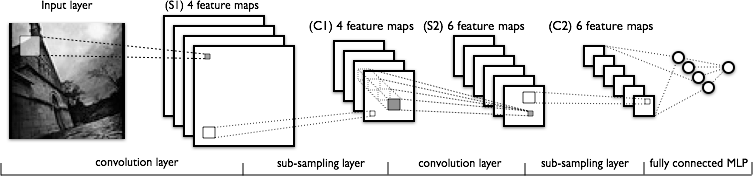
\includegraphics[width=0.8\textwidth]{lenet.png}
\caption{\label{fig:perceptron}Diagram of LeNet.}
\end{figure}

\section{Spatial Pyramid Match}

Spatial pyramid match\citep{lazebnik2006beyond} is used to classify high-level semantic attributes, based on low-level features. The method subdivides a image in several different levels of resolution and counts features falling in each spatial bin. It extends bags of features and derives spatial information from images.
\graphicspath{ {./Figures/} }
\begin{figure}[!htb]
\centering
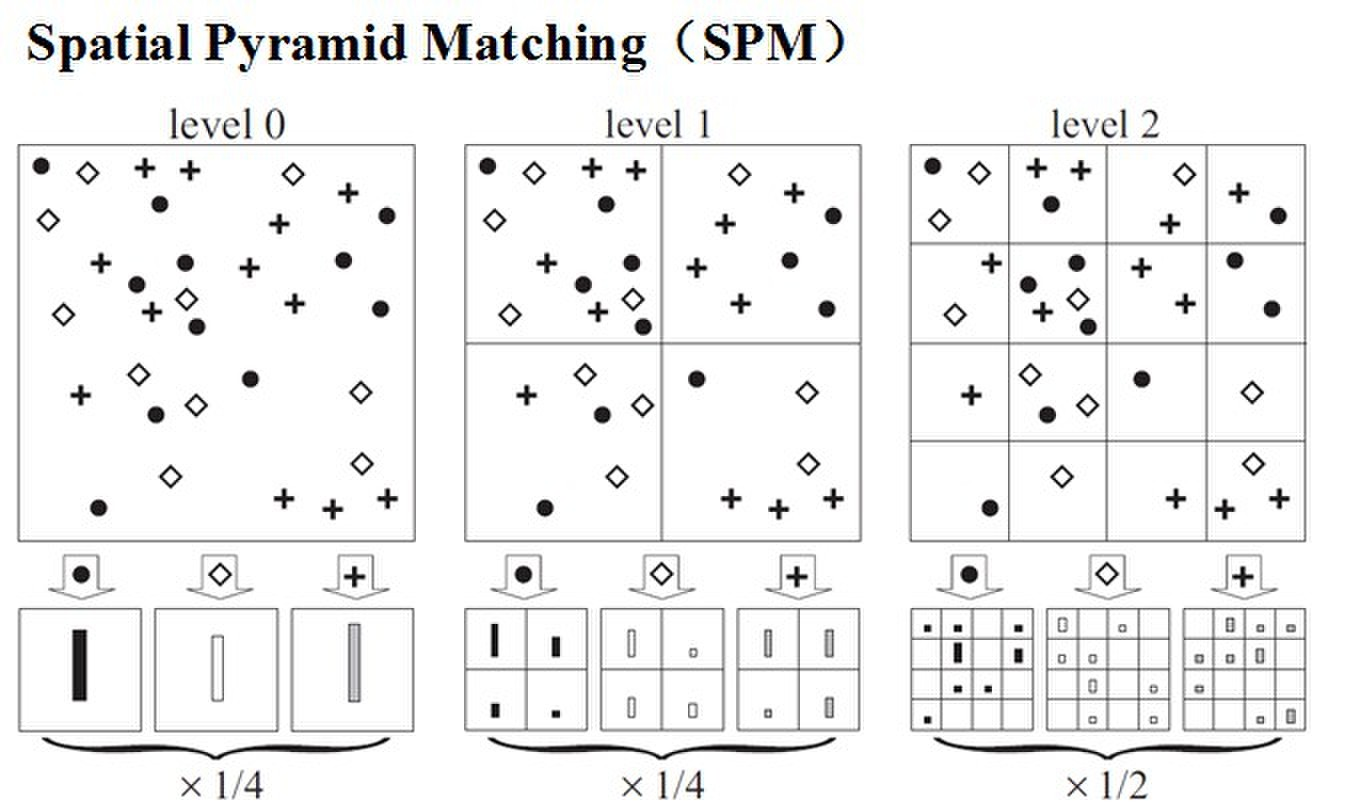
\includegraphics[width=0.8\textwidth]{spm.jpg}
\caption{\label{fig:perceptron}Diagram of Spatial Pyramid Match.}
\end{figure}

\section{Transfer Learning}

In machine learning literature, transfer learning\citep{pan2010survey} focuses on storing knowledge from one domain and applying it to a related problem. It has two benefits. One is saving time to build a model from scratch up. Another is saving effort to collect training data.

A domain with two components, a feature space and a marginal probability distribution, can be represented
\begin{equation}\label{eq:TransLearning}
D = \{ \chi, P(X) \}
\end{equation}
where $\chi$ is feature space and $P(X)$ is the marginal probability distribution. 
\graphicspath{ {./Figures/} }
\begin{figure}[!htb]
\centering
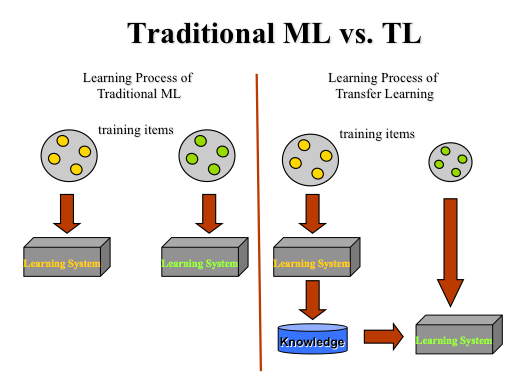
\includegraphics[width=0.8\textwidth]{MLvsTL.png}
\caption{\label{fig:perceptron}Diagram of Transfer Learning.}
\end{figure}
 % Background Theory and Related Work

% Chapter 2

\chapter{Methodology} % Write in your own chapter title
\label{Chapter3}
\lhead{Chapter 3. \emph{Approach of Weather Classification}}

\section{Dataset}

There are over 15 million labeled images in ImageNet database belonging to about 22,000 categories. The images were collected from the Internet and labeled manually. From 2010, an annual competition named the ImageNet Large-Scale Visual REcognition Challenge (ILSVRC) has been held. The competition uses a subset of dataset which is 1000 images in 1000 categories. Totally, there are over 1 million training images and 50,000 validation images and 150,000 images for testing.
\graphicspath{ {./Figures/} }
\begin{figure}[!htb]
    \centering
	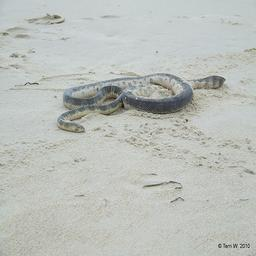
\includegraphics[width=0.4\textwidth]{ILSVRC2012_val_00000001.JPEG}
    \qquad
    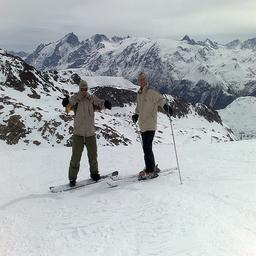
\includegraphics[width=0.4\textwidth]{ILSVRC2012_val_00000002.JPEG}
    \caption{2 Figures from ImageNet}%
    \label{fig:ImageNetExamples}%
\end{figure}

For weather dataset, it contains 10,000 images for two categories evenly, cloudy and sunny. They are from three sources, Sun Dataset\citep{russell2008labelme}, Labelme Dataset\citep{xiao2010sun} and Flickr. They were classified manually and similar images are removed. There are no unambiguous images.
\graphicspath{ {./Figures/} }
\begin{figure}[!htb]
    \centering
	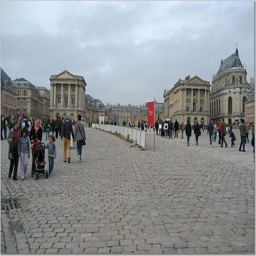
\includegraphics[width=0.4\textwidth]{cloudy_0001.png}
    \qquad
    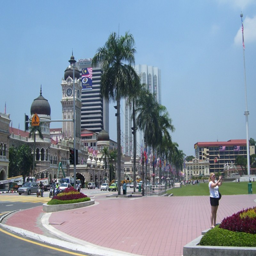
\includegraphics[width=0.4\textwidth]{sunny_0003.png}
    \caption{2 Figures from Weather Dataset}%
    \label{fig:WeatherExamples}%
\end{figure}

The two datasets are different. ImageNet dataset is for object classification and weather dataset is for scenes classification. Because the two datasets consists of different resolution images, we have to resize them to a fixed resolution of $256x256$ for constant dimension input for neural networks. To train the model with ImageNet images, we resize shorter side of images to length 256 and then cropped out a $256x256$ image from center.


\section{Convolutional Neural Networks Architecture}

Due to the significant performance of AlexNet \citep{krizhevsky2012imagenet} deep convolutional neural networks, we train a model based on it. The architecture of the network has seven hidden adaptive layers-five convolutional and two fully connected layers.
\begin{figure}[!htb]
    \centering
	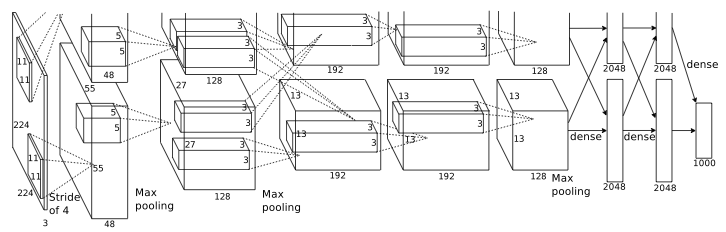
\includegraphics[width=0.8\textwidth]{AlexNet.png}
    \caption{Architecture of AlexNet}%
    \label{fig:ImageNetArch}%
\end{figure}
The network is very deep and the early layers are split over on two GPUs. It is able to give $62.5\%$ accuracy rates with one prediction and $83\%$ accuracy rates with five predictions.

The network replaces each neuron's outputs nonlinearity function $f$ from $f(x) = tanh(x)$ or $f(x) = (1 + e^{-x})^(-1)$ to Rectified Linear Units(RELUs)\citep{nair2010rectified} which can accelerate learning speed several times faster than $tanh$ function. 

In the network, there are three types of layers and they play different roles in the model. The input data dimension is $224x224x3$ which means the raw pixel value stored in a width 224, height 224 and with three color channels R,G,B matrix. In the first convolutional layer, there are 98 kernel of size $11x11x3$ with stride size 4 and outputs are 96 neurons. A max pooling layer downsamples the spatial dimensions. The second convolutional layer filters output of previous pooling layer with kernel size $5x5x48$. The third convolutiona layer owns 384 kernels of $3x3x256$ and receives outputs of the second convolutional layer. The fourth convolutional layer has 384 kernels of size $3x3x192$ and the last convolutional layer has 256 kernels of size $3x3x192$. Each fully connected layers have 4096 units. At the end of network, there is a softmax layer with 1000 outputs.

\section{Data Argument}

The model has about 60 million neurons, and it is essential to avoid overfitting. One of methods is to do data argument. Dataset is artificially enlarged via image transformations and horizontal reflections. For each $256x256$ image, the network extracts five $224x224$ patches from four corners and center and reflects them horizontally. Hence, there are 10 patches for 1 image in total. 

\section{Spatial Pyramid Pooling}

To improve the capability of generalization, a spatial pyramid pooling layer is deployed behind the fifth convolutional layer. A set of bin sizes are set to discern different size local information from output of the fifth convolutional layer.  A sliding window pooling  is implemented on the feature maps after the fifth convolutional layer. Assuming dimension of feature map is $axa$ and bin size is $n$, each window size is $\lceil a/n \rceil$ and stride size is $\lfloor a/n \rfloor$ where $\lceil \rceil$ and $\lfloor \rfloor$ denote ceiling and flooring operations. For $l$ level pyramid, there are $l$ spatial pyramid pooling layers, The the $l$ layers will be concatenated into a fully connected layer. The bin sizes are 1, 2, 3 and 6.

\begin{figure}[!htb]
    \centering
	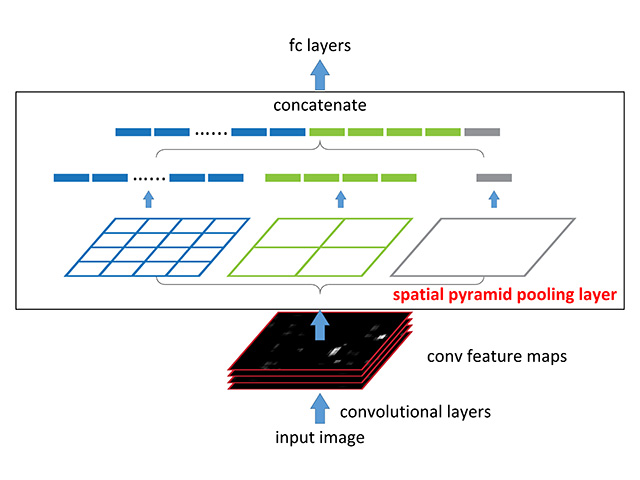
\includegraphics[width=0.8\textwidth]{sppnet.jpg}
    \caption{Diagram of Spatial Pyramid Pooling layer}%
    \label{fig:sppnet}%
\end{figure}

With implementing spatial pyramid pooling layers in convolutional neural networks, all contribution of different scales are considered. 

\section{Learning Rates}















 % Methodology

% Chapter 4

\chapter{Experiment} % Write in your own chapter title
\label{Chapter4}
\lhead{Chapter 4. \emph{Experiment}}

We set up experiment environment on a desktop which has hardware i7 CPU, 8G RAM and a GeForce GTX 770 and software operation system Ubuntu Linux 14.04. We train models in Caffe\citep{jia2014caffe} which is a open source framework and develop spatial pyramid pooling layer in the architecture.

\section{Training Neural Network}

We trained model with the 1000-category ImageNet2012 on deep learning framework CaffeNet~\cite{jia2014caffe} on a  We use the base network architecture of fast(smaller) model~\cite{ZeilerF13} which achieved an excellent result in 2013 ImageNet Competition. We implement SPP with CUDA C language and deploy them before the first fully-connected layer.

In experiment, a subset of ImageNet dataset, which contains 1.2 million labelled high-resolution images depicting 1000 object categories for training and 50,000 validation images, is used as training dataset. ImageNet contains of multi-scale and some grey images which are converted to a constant input dimensionality. Then images are resized to $256x256$. And for grey images, they are combined it triple to minic a RGB image. Model is trained on the raw RGB values of pixels. Activation function is chosen  Rectified Linear Units(ReLUs), which allows for faster and effective training of deep neural networks.

\begin{equation}\label{eq:ReLU}
f(x) = max(0, x)
\end{equation}

The network model \ref{eq:NetPara} is trained with stochastic gradient descent as backpropagation learning rule, with a batch size of 128, and momentum of 0.9. The weights are initialized from a $0$ mean Gaussian distribution with standard deviation 0.01 in each layer. The neuron biases, in the $Conv_{2}$, $Conv_{4}$, $Conv_{5}$ and fully connected layers, are initialized with the constant 1, while biases in other layers are initialized with constant 0.

The learning rates are set equally for all layers. It was initialized at 0.01 and decreases with stepdown policy which means that it would drop by a factor of 10 after 100000 iteration. In total, the learning rate drops 3 times and accuracy stops after 370K iterations. 

The training was regularised by dropout and weight decay. Dropout regularisation is implemented in the first two fully-connected layers and dropout ratio is set to 0.5. The neurons which are dropped out output zero and do not participate in backpropagation. Therefore, the neural network samples a different architecture each time. It greatly decreases complex co-adaptations of neurons because a neuron cannot depend on the existence of distinct other neurons. For weight decay $\epsilon$, it is set to 0.0005 which means , after each weight update, the new weight is shrunk according to 
\begin{equation}\label{eq:ffEq}
w^{new} = w^{old}(1 - \epsilon)
\end{equation}

\section{Fine-tuning Model}

As mentioned previously, the CNN network is pre-trained with aim of classifying objects in images. However, the target task is to classify weather scene and the pre-trained model contains more than 60 million parameters which are too high for training target model from scratch up, because the target dataset has only 10000 images in total. With the excellent accuracy achieved from previous works about transfer learning, it is a good approach to fine-tune previous model. The previous model does a job to classify 1000 categories and the target model does for two class classification. 

Fine-tuning transfers weights of each layers in previous model to new one except the last fully connected layer. The last layer is taken over by a new one which contains the same amount of neurons as class number in the dataset, say two, and is initialized with random weights. One advantage of fine-tune is that it highly reduces the probability of overfitting  while training with small dataset. The other advantage is the existing weights are close to optimal values and the gradient descent algorithm can converge quickly.

In the problem, we want to classify sunny and cloudy images, then the last layer of the previous architecture, $fc8$, is taken place by a layer with two neurons, one for sunny and one for cloudy. The model, trained using ILSVRC2012 dataset, is used to initialize most weights in the neural network for the fine-tuning experiment. At the same time, $1000$ images are used to evaluate model. The model is fine-tuned in $10000$ iterations which means that total training images are fed into CNN $\frac{128x10000}{9000}=142$ times. The initial base learning rate is 0.001 and the rate is divided by 10 every 10 epochs. Because the weights in $fc8$ are randomly initialized which means they are not close to final optimization value, the learning rate of $fc8$ is 10 times of the base learning rate in order to converge faster.

To minimise risk of overfitting, data augmentation is introduced in to experiment. Different version of patches are generated from each image via simple transformations, for example flipping and cropping. Some practical methods have been implemented and increase accuracy \citep{krizhevsky2012imagenet}. We do this job by increasing the spatial generalization capability of the model  by cropping 5 different patches from four corners and center of images, and flipping them. Totally, we generate 10 different images with the same label.

\section{Companion Experimental}

To compare the performance of fine-tuned model, we do some a experiment with other method. We use a pre-trained model with AlexNet architecture and extract features from fc7. Then we apply SVM on the features and learn a classifier to do weather classification.

\section{Experimental Result}

The results in table\ref{ExpRes} shows that supervised pre-training model have excellent generalization capability. 

\begin{table}[h]
\begin{center}
    \begin{tabular}{| c | c | c | c | c |}
    \hline
    Methods & CNN+SVM & SPP+SVM & Finetune on CNN & Finetune on SPP  \\ \hline
    Accuracy & $84.8\%$ & $82.1\%$ & $93.1\%$ & $93.98\%$ \\ \hline
    \end{tabular}
    \caption{CNN means with original trained model, SPP means model deployed with spatial pyramid pooling layer}
    \label{ExpRes}
\end{center}
\end{table}

The fine-tuning process is very quick, and accuracy rate convergences to over $90\%$. 
After 12 epoch, the accuracy rate exceeds $90\%$. 
\graphicspath{ {./Figures/} }
\begin{figure}[!htb]
    \centering
	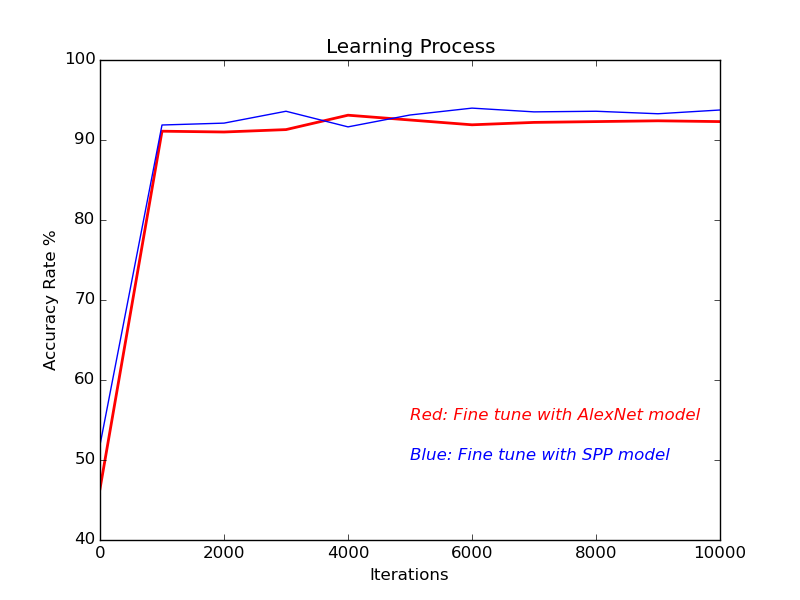
\includegraphics[width=0.8\textwidth]{FinetuneAccuracy.png}
    \caption{Finetune Process}%
    \label{fig:finetuneprocess}%
\end{figure}

No single image dataset can totally capture variation in natural images, so even ImageNet is biased in some fields. Then pre-training may be make the CNN to overfit and then damage model generalization capability. To learning the process of ImageNet pre-training, we look into the effect of pre-training period on generalization performance with and without fine-tuning. In figure \ref{fig:finetuneprocess}, we can find that longer pre-training improves performance.

To have a more detailed information of fine-tuning process, we can have a closer look at training loss. We plot the curve of first 200 iterations and loss value.

\begin{figure}[!htb]
    \centering
	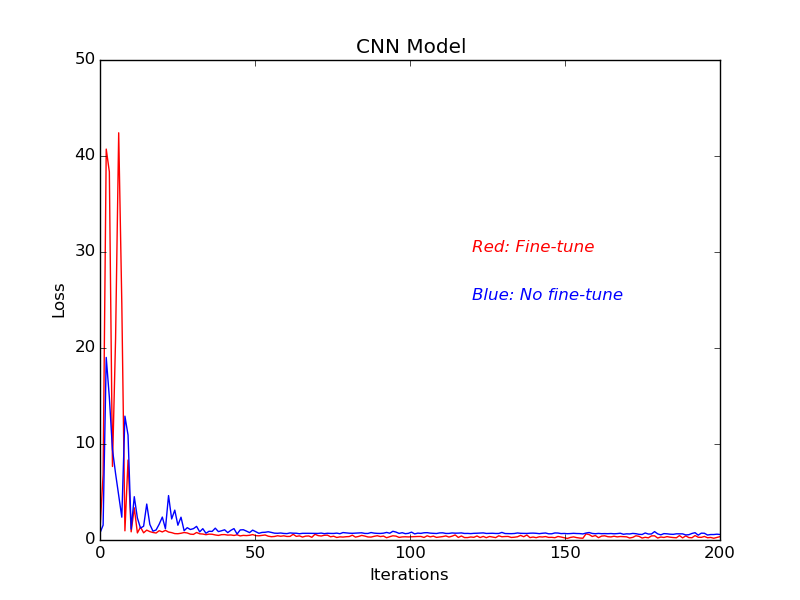
\includegraphics[width=0.4\textwidth]{finetuneCNNProcess.png}
	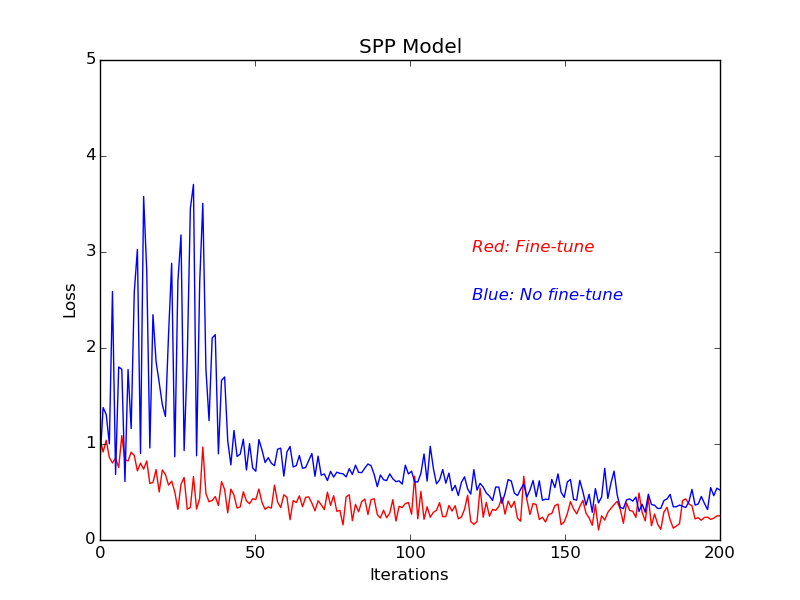
\includegraphics[width=0.4\textwidth]{finetuneSPPProcess.png}
    \caption{Finetune Process}%
    \label{fig:FTvsSC}%
\end{figure}

From figure \ref{fig:FTvsSC}, we can find that the fine-tuning procedure produces a more smooth loss function curve and ceases with a better loss. In the left figure, the loss value of fine tune procedure is higher than no fine tune process at the beginning, then it shrinks sharply and keeps lower. In the other figure, we can find that starting loss value are both less than in the left figure. And the loss values of fine tune are less than no fine tune process. We can conclude that generally fine tune is a effective approach to reduce loss value and fine tune on SPP model can achieve a better result than CNN model.

\section{Architecture Analysis}

Although CNNs have excellent performance in computer vision field, there is still a long way to understand insight working mechanism. In order to have more insight about the reason why deep layers can increase performance of visual sentiment classification, we will do some analysis on fine-tuned network.

The outputs of each layers have been treated as visual descriptors \citep{razavian2014cnn}, while the vectors are composed by outputs of neurons in previous layer. While the lower layers encode low-level features, top layers have been used to capture high-level information. In other words, we can train classifiers basing on features extracted from each layer.

In fully-connected layer, units can be represented as d dimensional vectors, and no further manipulation is needed. The layer takes all outputs of previous layer ,for example CONV, POOL, NORM,whose feature maps are multidimensional, and flats the feature maps into d dimensional vectors. The outputs of fully connected layer are feed into a classifier. Two types of linear classifiers are used. They are linear Support Vector Machine and Softmax.

 % Experiment 1

% Chapter 5

\chapter{Introduction} % Write in your own chapter title
\label{Chapter5}
\lhead{Chapter 5. \emph{Introduction}} % Multi-label classification


\section{Overview}

In machine learning literature, multi-label classification is a variant of the classification problem in which each instance has several labels. In general, the task of multi-label learning is to find a model that can maps inputs \textbf{x} to binary vector \textbf{y}. While it is different with multi-class classfication in terms of the later one scalars outputs in classification problem.

\graphicspath{ {./Figures/} }
\begin{figure}[!htb]
    \centering
	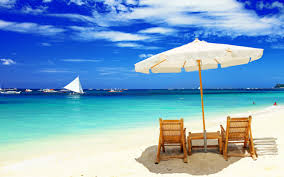
\includegraphics[width=0.8\textwidth]{beach.jpg}
    \caption{Example Image}%
    \label{fig:MultilableImage}%
\end{figure}

The difference between single-label classification and multi-label classification is the outputs of datasets.
In Figure \ref{fig:MultilableImage}, we can classify it as a picture of a beach in classification literature $\in \{Yes, No\}$. In multi-label literature, we can tag sea, beach, chairs, sky, cloud for the picture $\in \{beach, sea, chairs, sand\}$.

\begin{table}
\centering
\begin{tabular}{|c c c c c | c c c c|}
\hline
$X_{1}$ & $X_{2}$ &  $X_{3}$ & $X_{4}$ & $X_{5}$ & $Y_{1}$ & $Y_{2}$ & $Y_{3}$ & $Y_{4}$ \\
\hline
1 & 0.4 & 0.2 & 0 & 1 & 0 & 1 & 1 & 0 \\
0 & 0.2 & 0.6 & 1 & 1 & 1 & 0 & 1 & 0 \\
0 & 0.5 & 0.8 & 1 & 1 & 0 & 0 & 1 & 0 \\
1 & 0.1 & 0.4 & 0 & 1 & 1 & 1 & 1 & 0 \\
1 & 0.8 & 0.2 & 0 & 1 & 0 & 1 & 1 & 0 \\
\hline
0 & 0.5 & 0.3 & 1 & 1 & ? & ? & ? & ? \\
\hline
\end{tabular}
\caption{Multilabel $Y_{1},...,Y_{L} \in 2^L$}
\ref{tab:MultilabelTable}
\end{table}

In general, there exists two main approaches of tackling the multi-label classification problem. One transfers a multi-label problem into a set of binary classification problems which can be handled by a set of binary classifiers. The other one applies algorithms to complete multi-label classification. 

Several problem transformation methods can be applied to multi-label classification. A baseline method, named the binary relevance method\citep{read2011classifier}, trains one binary classifier for each label independently. Depending on the results of the classifiers, the combined model predicts all labels for an unseen sample. The method divides the problem into multiple binary works which has something in common with the one-vs-all method for multi-class classification. Problem transformation benefits from scalability and flexibility because single-label classifier can be implemented to job. Support Vector Machine, Naive Bayes, $k$ Nearest Neighbor have been used in the method\citep{read2011classifier}.

There are some other transformation methods, for instance label powerset transformation. The method builds up one binary classifier for each label combination verified in the training dataset\citep{tsoumakas2006multi}. The random $k$-labelsets algorithm\citep{tsoumakas2007random} utilizes multiple label powerset classifier which is trained on a random sub dataset of the labels. A voting scheme is used to predict unseen samples via a ensemble method.

Multilayer neural network can be trained to learn a model from multi-label examples. We will generate a 3 labels dataset and use a 2 layer network to do classification.

\section{Multi-Label Learning}
Let $X = R^d$ represent the domain of dataset and let $Y = {1,2,..,L}$ be the finite set of labels. Given that we have a set of training dataset $T = {(x_{1},Y_{1}),(x_{2},Y_{2}),...,(x_{l},Y_{l})} (x_{i} \in X, Y_{i} \subset Y)$ which are extracted from an unknown distribution $D$. Our target of task is to learn a multi-label classifier $h: X \to 2^y $ via optimizing specific evaluation metric. However, instead of learning a multi-label classifier, we will learn a function $f$ while $f(X) \to R^d$. Supposing that a high performance classifier can output a closer subset for labels in $Y_{i}$ than those missing or exceeding in $Y_{i}$, which means $f(x_{i}, y_{1}) > f(x_{i}, y_{2})$ if $y_{1} \in Y{i}$ and $y_{2} \notin Y{i}$. We can transfer real valued function $f(\cdot , \cdot)$ to a ranking function $r(\cdot , \cdot)$ that maps the outputs of $f(x_{i}, y_{1})$ to any $y \in Y$ if $f(x_{i}, y_{1}) > f(x_{i}, y_{2})$. It is worth noting that the multi-label classifier $h(\cdot)$ can be derived from the function $f(\cdot , \cdot)$ where $h(x_{i}) = {y|f(x_{i}, y) > t(x_{i}), y \in Y}$, and $t(\cdot)$ is a threshold function.

Single-label and multi-class classification can be regarded as two degenerated variants of multi-label learning problem if each sample has only one single label. However, multi-label problem is much more difficult than traditional single-label problems because of high dimensional output space. For example, the number of label sets increases exponentially with increasing number of class labels. If there are $10$ class labels for dataset, there are $2^20$ possible label sets maximun.

The challenge of huge combination of output labels is hard to overcome. One of methods is to investigate dependency among labels. For example, if an image labelled with $castle$, it would be highly labelled with $brick$ and $mountain$. A movie which is labelled with $comedy$ is unlikely related to a $documentary$. Therefore, successful exploitation of the label correlations is regarded as an effective approach to high accuracy multi-label learning process. There are three categories, based on the order of correlation of labels, for existing strategies to find the relation between labels. They are first order strategy, second order strategy and high-order strategy. 

The first order strategy treats label by label independently and ignores correlation between labels. It can be regarded as decomposing a multi-label learning problem into a set of binary classification problems based on each label. The method benefits from simple computation and high efficiency. However, accuracy could be suboptimal because of ignoring the correlations of labels.

The second order strategy considers pairwise relations between labels, for example, interaction between any pair of labels, or the ranking between related labels and unrelated labels. The method can help to achieve good generalization performance because the label correlations are investigated in some extent. In real world, there are higher order correlations than second order assumption in many applications.

The high order strategy investigates more than $2$ order correlations among labels which can be the influences on each label or addressing connections among sub space of output labels. It is obvious that high order strategy has the strongest model capabilities than previous two strategies on the cost of complexity and intensive computation.

\section{Evaluation Metrics}

In supervised learning settings, different metrics, like accuracy and area under the ROC curve, are used to evaluate the generalization performance of learning system. In multi-label learning, evaluating performance is more complicated  than single-label problems with the increasing number of labels simultaneously. Therefore, two main types of evaluation methods are implemented in multi-label learning, say example-based metrics\citep{ghamrawi2005collective} and label-metrics\citep{tsoumakas2007random}.

The two types of metrics evaluate the outputs of classifier from different perspective. Given that $S = {(x_{i}, Y_{i})}$ is the test instance and $h(\cdot)$ is the learned multi-label classifier. Example-based metrics achieve all class labels of each test example, and then compute the mean value of test set to evaluate generalization performance. Compared to considering all class labels simultaneously, label-based metrics evaluate performance by treating each class label separately and computing macro/micro-averaged value of all class labels.

In a supervised classification problem, there have a ground truth output and a predicted output of test instance. So the results of each test instance can be be assigned to one of the four categories:
\begin{itemize}
\item True Positive (TP) - label is positive and prediction is also positive
\item True Negative (TN) - label is negative and prediction is also negative
\item False Positive (FP) - label is negative but prediction is positive
\item False Negative (FN) - label is positive but prediction is negative
\end{itemize}

Here we define a set $D$ of $N$ instances and $Y_{i}$ to be a family of ground truth label sets and $P_{i} = h(x_{i})$ to be a family of predicted label set. The set of all unique labels is
\begin{equation}\label{eq:UniLabel}
L = \bigcup_{i=0}^{N-1} L_{i}
\end{equation}
While the definition of indicator function $I_{A}$ on a set $A$ is presented as
\begin{equation}\label{eq:IndicatorFunc}
I_{A}(x) =
  \begin{cases}
    1       & \quad \text{if } x \in A\\
    0  & \quad \text{otherwise}\\
  \end{cases}
\end{equation}

\subsection{Example-based Metrics}

\textbf{Hamming Loss} evaluates performance via counting the number of misclassification labels. The smaller value of hamming loss, the better performance.
\begin{equation}\label{eq:HammingLoss}
\frac{1}{N \cdot \left|L\right|} \sum_{i=0}^{N - 1} \left|L_i\right| + \left|P_i\right| - 2\left|L_i
          \cap P_i\right|
\end{equation}

\textbf{Subset Accuracy} evaluates the fraction of correctly predicted instance while the predicted label set is identical to the ground truth label set. It is equivalent to traditional accuracy metric.
\begin{equation}\label{eq:SubsetAcu}
\frac{1}{N} \sum_{i=0}^{N-1} I_{\{L_i\}}(P_i)
\end{equation}

\textbf{Precision} is defined as
\begin{equation}\label{eq:Precision}
\frac{1}{N} \sum_{i=0}^{N-1} \frac{\left|L_i \cap P_i\right|}{\left|P_i\right|}
\end{equation}

\textbf{Recall} is defined as
\begin{equation}\label{eq:Recall}
\frac{1}{N} \sum_{i=0}^{N-1} \frac{\left|L_i \cap P_i\right|}{\left|L_i\right|}
\end{equation}

\textbf{Accuracy} is defined as
\begin{equation}\label{eq:Accuracy}
\frac{1}{N} \sum_{i=0}^{N - 1} \frac{\left|L_i \cap P_i \right|}
        {\left|L_i\right| + \left|P_i\right| - \left|L_i \cap P_i \right|}
\end{equation}

\textbf{F1 Measure} is an integrated version combined by harmonic mean of \textbf{Precision} and \textbf{Recall}. 
\begin{equation}\label{eq:Accuracy}
\frac{1}{N} \sum_{i=0}^{N-1} 2 \frac{\left|P_i \cap L_i\right|}{\left|P_i\right| \cdot \left|L_i\right|}
\end{equation}

\subsection{Label-based Metrics}

\textbf{Macro Precision} (precision averaged across all labels) is defined as
\begin{equation}\label{eq:MacroPrecision}
PPV(\ell)=\frac{TP}{TP + FP}=
          \frac{\sum_{i=0}^{N-1} I_{P_i}(\ell) \cdot I_{L_i}(\ell)}
          {\sum_{i=0}^{N-1} I_{P_i}(\ell)}
\end{equation}

\textbf{Macro Recall} (recall averaged across all labels) is defined as
\begin{equation}\label{eq:MacroRecall}
TPR(\ell)=\frac{TP}{P}=
          \frac{\sum_{i=0}^{N-1} I_{P_i}(\ell) \cdot I_{L_i}(\ell)}
          {\sum_{i=0}^{N-1} I_{L_i}(\ell)}
\end{equation}

\textbf{F1 Measure by label} is the harmonic mean between \textbf{Precision} and \textbf{Recall}. 
\begin{equation}\label{eq:LabelAccuracy}
F1(\ell) = 2
                            \cdot \left(\frac{PPV(\ell) \cdot TPR(\ell)}
                            {PPV(\ell) + TPR(\ell)}\right)
\end{equation}

\textbf{Micro Precision} (precision averaged over all the example/label pairs) is defined as
\begin{equation}\label{eq:MicroPrecision}
\frac{TP}{TP + FP}=\frac{\sum_{i=0}^{N-1} \left|P_i \cap L_i\right|}
          {\sum_{i=0}^{N-1} \left|P_i \cap L_i\right| + \sum_{i=0}^{N-1} \left|P_i - L_i\right|}
\end{equation}

\textbf{Micro Recall} (recall averaged over all the example/label pairs) is defined as
\begin{equation}\label{eq:MicroRecall}
\frac{TP}{TP + FN}=\frac{\sum_{i=0}^{N-1} \left|P_i \cap L_i\right|}
        {\sum_{i=0}^{N-1} \left|P_i \cap L_i\right| + \sum_{i=0}^{N-1} \left|L_i - P_i\right|}
\end{equation}

\textbf{Micro F1 Measure by label} is the harmonic mean between \textbf{Micro Precision} and \textbf{Micro Recall}. 
\begin{equation}\label{eq:LabelMicroAccuracy}
2 \cdot \frac{TP}{2 \cdot TP + FP + FN}=2 \cdot \frac{\sum_{i=0}^{N-1} \left|P_i \cap L_i\right|}{2 \cdot
        \sum_{i=0}^{N-1} \left|P_i \cap L_i\right| + \sum_{i=0}^{N-1} \left|L_i - P_i\right| + \sum_{i=0}^{N-1}
        \left|P_i - L_i\right|}
\end{equation}

For the label-based metrics, the larger the metrics value means the higher generalization performance.

With the previous metrics, there are diverse methods to evaluate model generalization performance. In most multi-label training, learning algorithms optimize one of the metrics. To make evaluation fair and precise, the learning algorithms should be tested on different metrics to evaluate performance to avoid bias.

Most multi-label metrics are non-convex and discrete, most algorithms turn to optimize alternative multi-label metrics. Recent some researcher study the consistency of multi-label learning\citep{gao2013consistency}, for example, figuring if the loss of classifier converges to the Bayes loss while increasing training set size.

\section{Loss Function}

To adapt a neural network handling single-label instances to multi-label instances, we need to design a specific loss function instead of squared error loss function to track the characteristics of multi-label learning and some revision of stochastic gradient descent. 

\section{Artificial Neural Networks}



\section{Weather Classification}




 % Multilable Introduction

% Chapter 6

\chapter{Multi-lable Classification Methodology} % Write in your own chapter title
\label{Chapter6}
\lhead{Chapter 6. \emph{Methodology}}

\section{Artificial Dataset}

To demonstrate the approach, the dataset, named color detector, is created artificially. To each image, it has three labels for representing colour, $red$, $green$ and $blue$. If an image is red hue, it has a label for $red$ and label values of $green$ and $blue$ are negative. The representation of colour combination follows colour wheels. If an image has a hue close to $purple$, it has positive labels for $red$ and $blue$, and negative label for $green$, and so on.
\graphicspath{ {./Figures/} }
\begin{figure}[!htb]
\centering
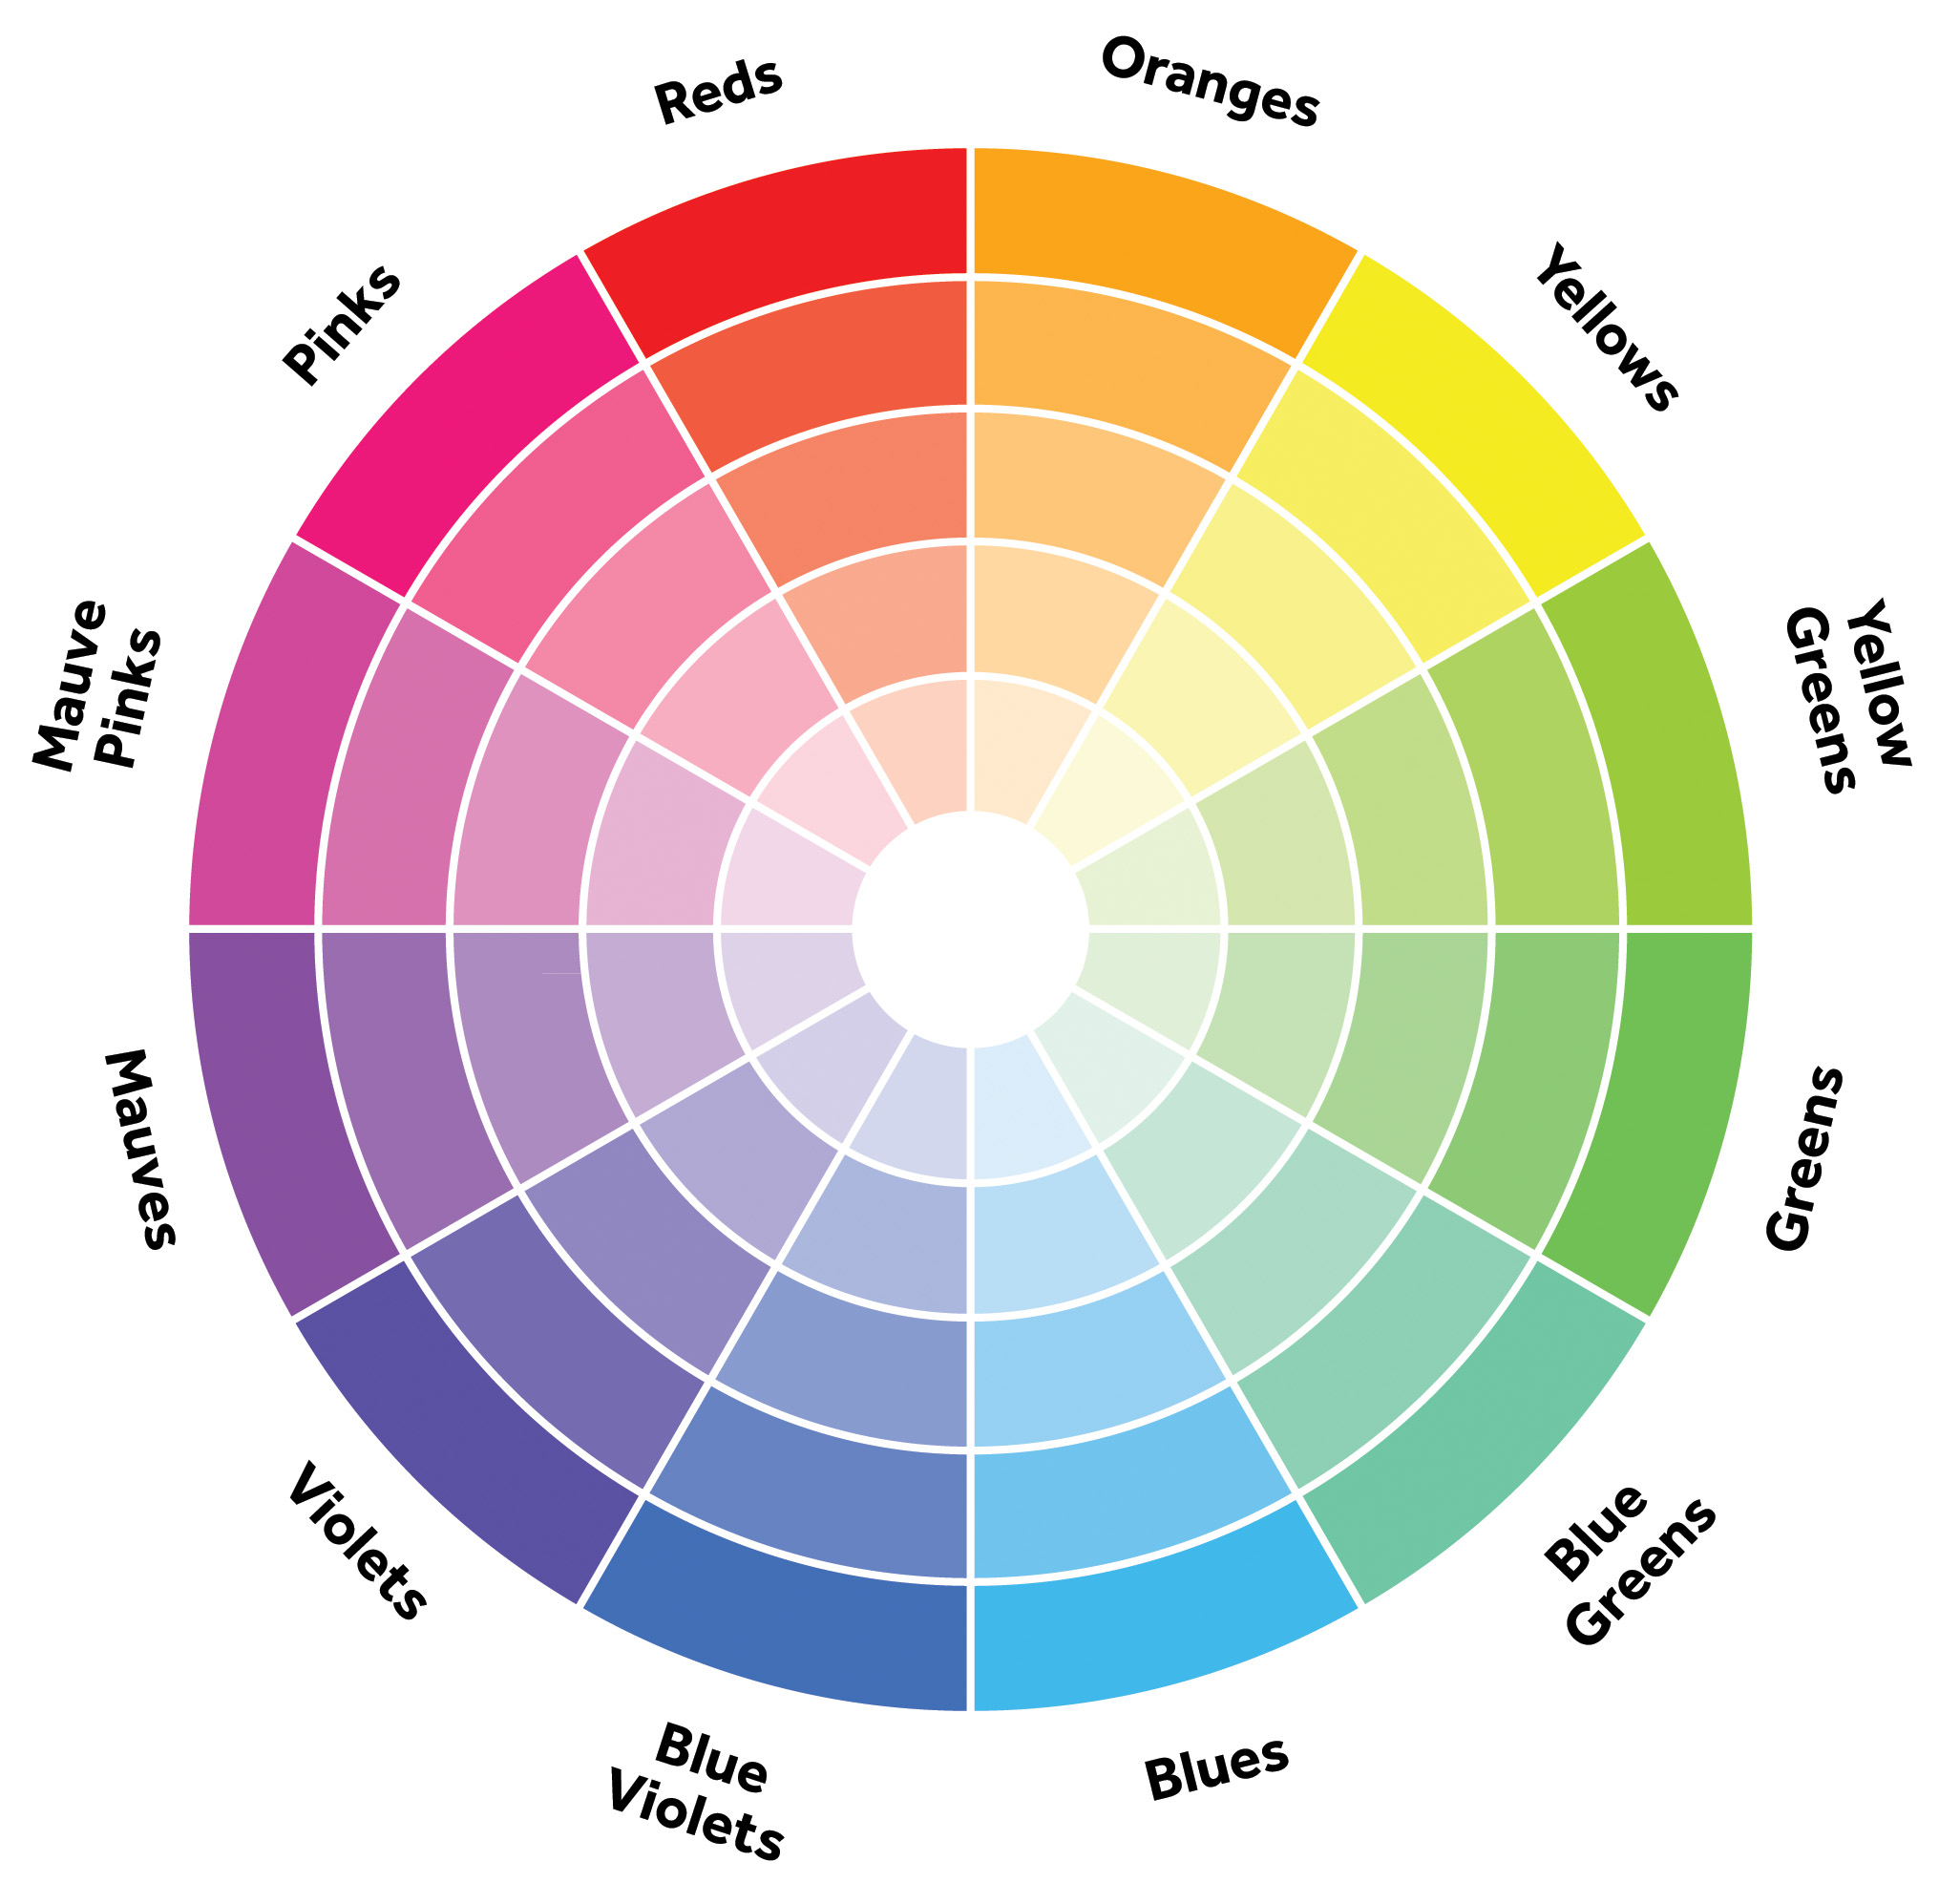
\includegraphics[scale=0.1]{color_wheel.jpg}
\caption{\label{fig:perceptron}Colour Wheel Diagram}
\end{figure}

For each sample $x_{i}$, it owns 3 labels ${y_{0},y_{1},y_{2}} y_{j} \in \{-1,1\}$ which represent $red$, $green$ and $blue$ respectively.

\subsection{Colour Generation}

To generate dataset artificially, we create $16x16$ size images and each image has $256$ pixels. For each pixel, we generate a random floating point number $h$ in the range $[0.0, 1.0)$ and use it as value for Hue via formulation.
\begin{equation}\label{eq:FormulationHue}
H = h + r * 0.4 - 0.2 (r \in [0.0,1.0))
\end{equation}
Where $r$ is another random floating point number. Then we generate 2 random floating point numbers as Saturation(S) and Value(V) values. We transform HSV values to RGB values and time $255$ for each pixel. Repeating the steps, we can get a $256$ pixels image. Because we get a RGB image via converting a HSV image, we compute RGB label value basing on previous $h$.

\graphicspath{ {./Figures/} }
\begin{figure}[!htb]
\centering     %%% not \center
\subfigure[L:-1 -1 1]{\label{fig:a}
\includegraphics[width=0.3\textwidth]{0}}
\subfigure[L:-1 1 1]{\label{fig:b}
\includegraphics[width=0.3\textwidth]{1}}
\subfigure[L:-1 1 -1]{\label{fig:c}
\includegraphics[width=0.3\textwidth]{3}}
\caption{Multi-label Samples. Left image is a blue one, middle one is green plus blue and right one is green.}
\end{figure}

The dataset contains $1000$ images in total. $960$ images are training samples and $40$ are test samples. 

\section{Artificial Neural Networks}

Artificial Neural networks are a good way to learn a nonlinear function which can be used to map samples to multi labels. At the first layer of a neural networks, neurons take raw dataset while the neurons in the last layer produce outputs. Among the first and the last layers, the middle layers are called hidden layers because they do not connect to external world. The 3-layer neural networks can represent any bounded degree polynomial under certain conditions\citep{barron1993universal}. The weights of neural networks are learned by algorithms deployed over training dataset. One of successful learning algorithms is the Backpropagation algorithm which updates weights by propagating errors caused by comparing network's prediction for each sample with actual target value.

To adapt classical neural networks, which handle simple-label classification, to classify multi-label samples, we need to modify two factors. One is to design a new error function which is fitting the characteristics of multi-label samples instead of single-label ones. The other is to find a moderate metric according to new designed error function.

















 % Multilable Methodology

%% Chapter 7

\chapter{Methodology} % Write in your own chapter title
\label{Chapter7}
\lhead{Chapter 7. \emph{Methodology}}

\section{Artificial Dataset}

The dataset, named a colour detector, is generated artificially. Each image has three labels to represent colours, $red$, $green$ and $blue$. If an image is a red hue only, it has a label for $red$ while the label values of $green$ and $blue$ are negative. The representation of colour combination follows colour wheels. If an image has a hue close to $purple$, it has positive labels for $red$ and $blue$, and negative label for $green$, and so on.
\graphicspath{ {./Figures/} }
\begin{figure}[!htb]
\centering
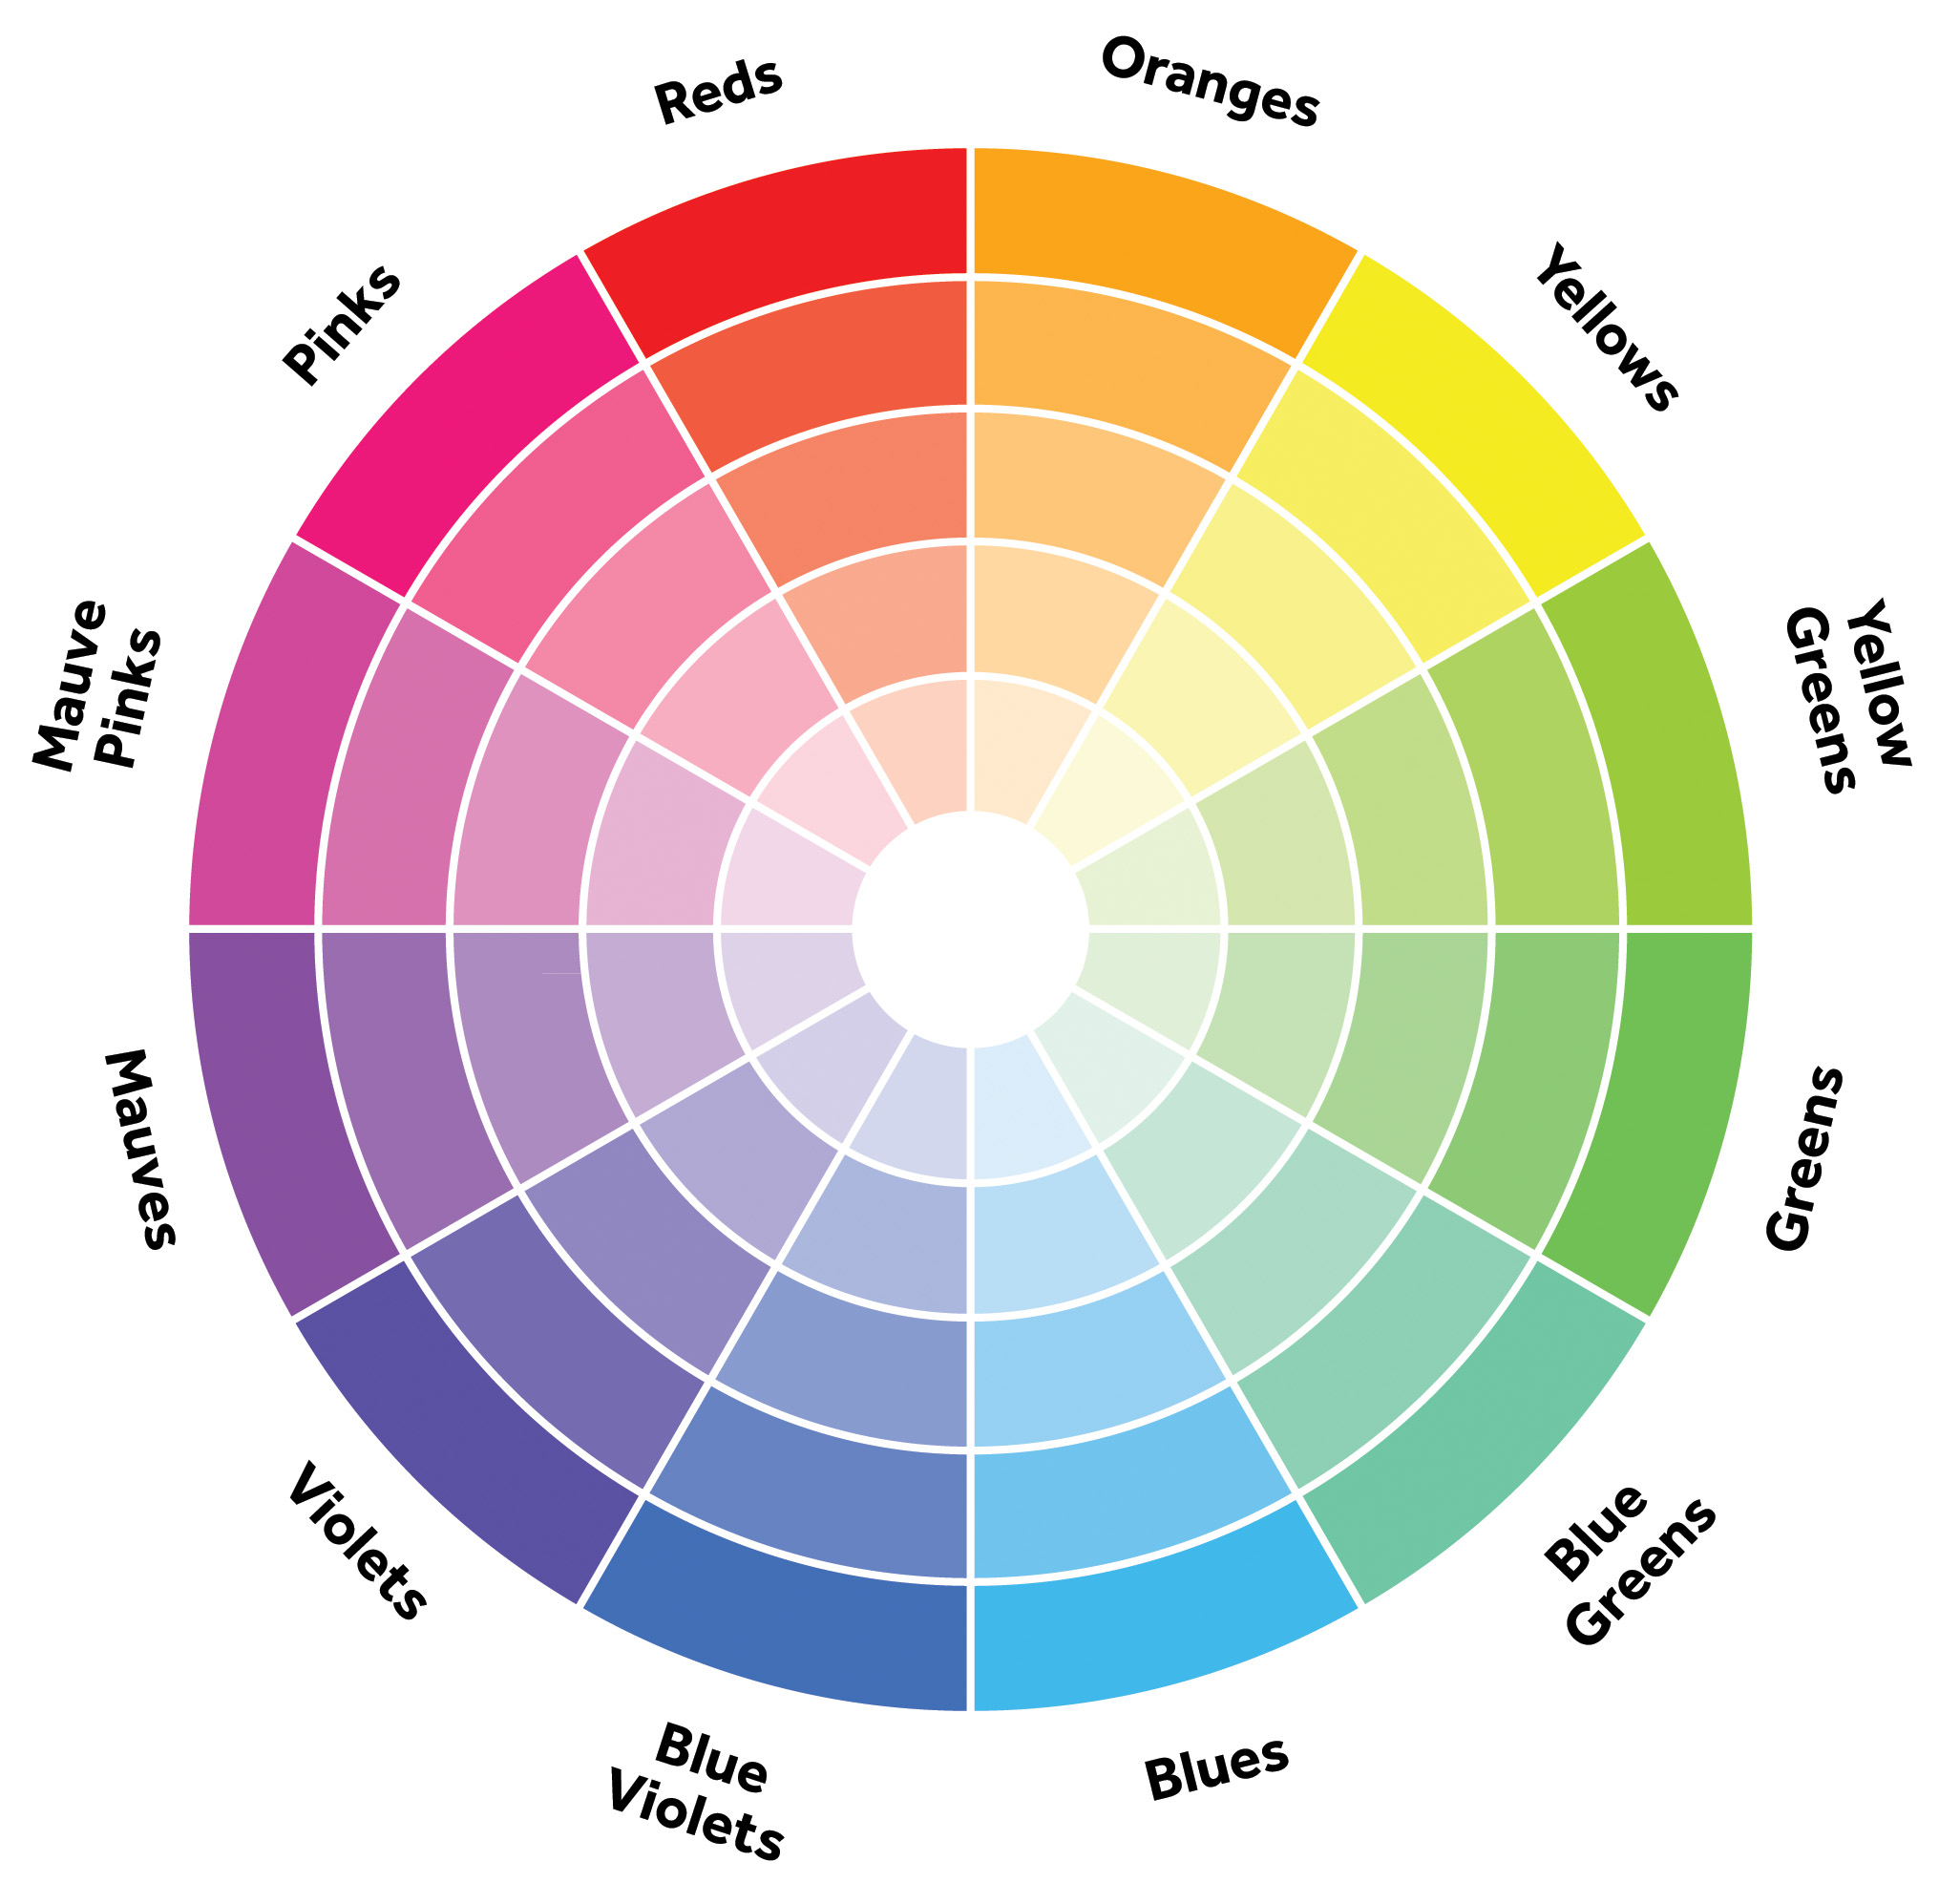
\includegraphics[scale=0.1]{color_wheel.jpg}
\caption{\label{fig:ColorWheel}Colour Wheel Diagram}
\end{figure}

For each sample $x_{i}$, it owns 3 labels ${y_{0},y_{1},y_{2}},  y_{j} \in \{-1,1\}$ which represent $red$, $green$ and $blue$ respectively.

\subsection{Generating images}

The RGB and HSV coordinate systems represent a geometric shape in colour space. The distance among colours contains little meaning. However, corresponding distance makes some intuitive sense and enable conversion possible between RGB coordinates and HSV coordinates.

The dataset consists of images with size $16x16$, so each image has $256$ pixels. To generate an image, I generate a random floating point number $h$ in the range $[0.0, 1.0)$ and use it as value for a hue via formulation.
\begin{equation}\label{eq:FormulationHue}
H = h + r * 0.4 - 0.2 (r \in [0.0,1.0))
\end{equation}
Where $r$ is another random floating point number. We generate 2 random floating point numbers for Saturation(S) and Value(V) values. The HSV values are converted to the RGB values and timed $255$ for each pixel. Following that, an image with $256$ pixels is generated. Because a RGB image is converted to a HSV image, the label values are based on the previous value $h$.

\graphicspath{ {./Figures/RGBhist/} }
\begin{figure}[!htb]
\centering     %%% not \center
\subfigure[Label:1 -1 1]{
\includegraphics[width=0.2\textwidth]{0}}
\subfigure{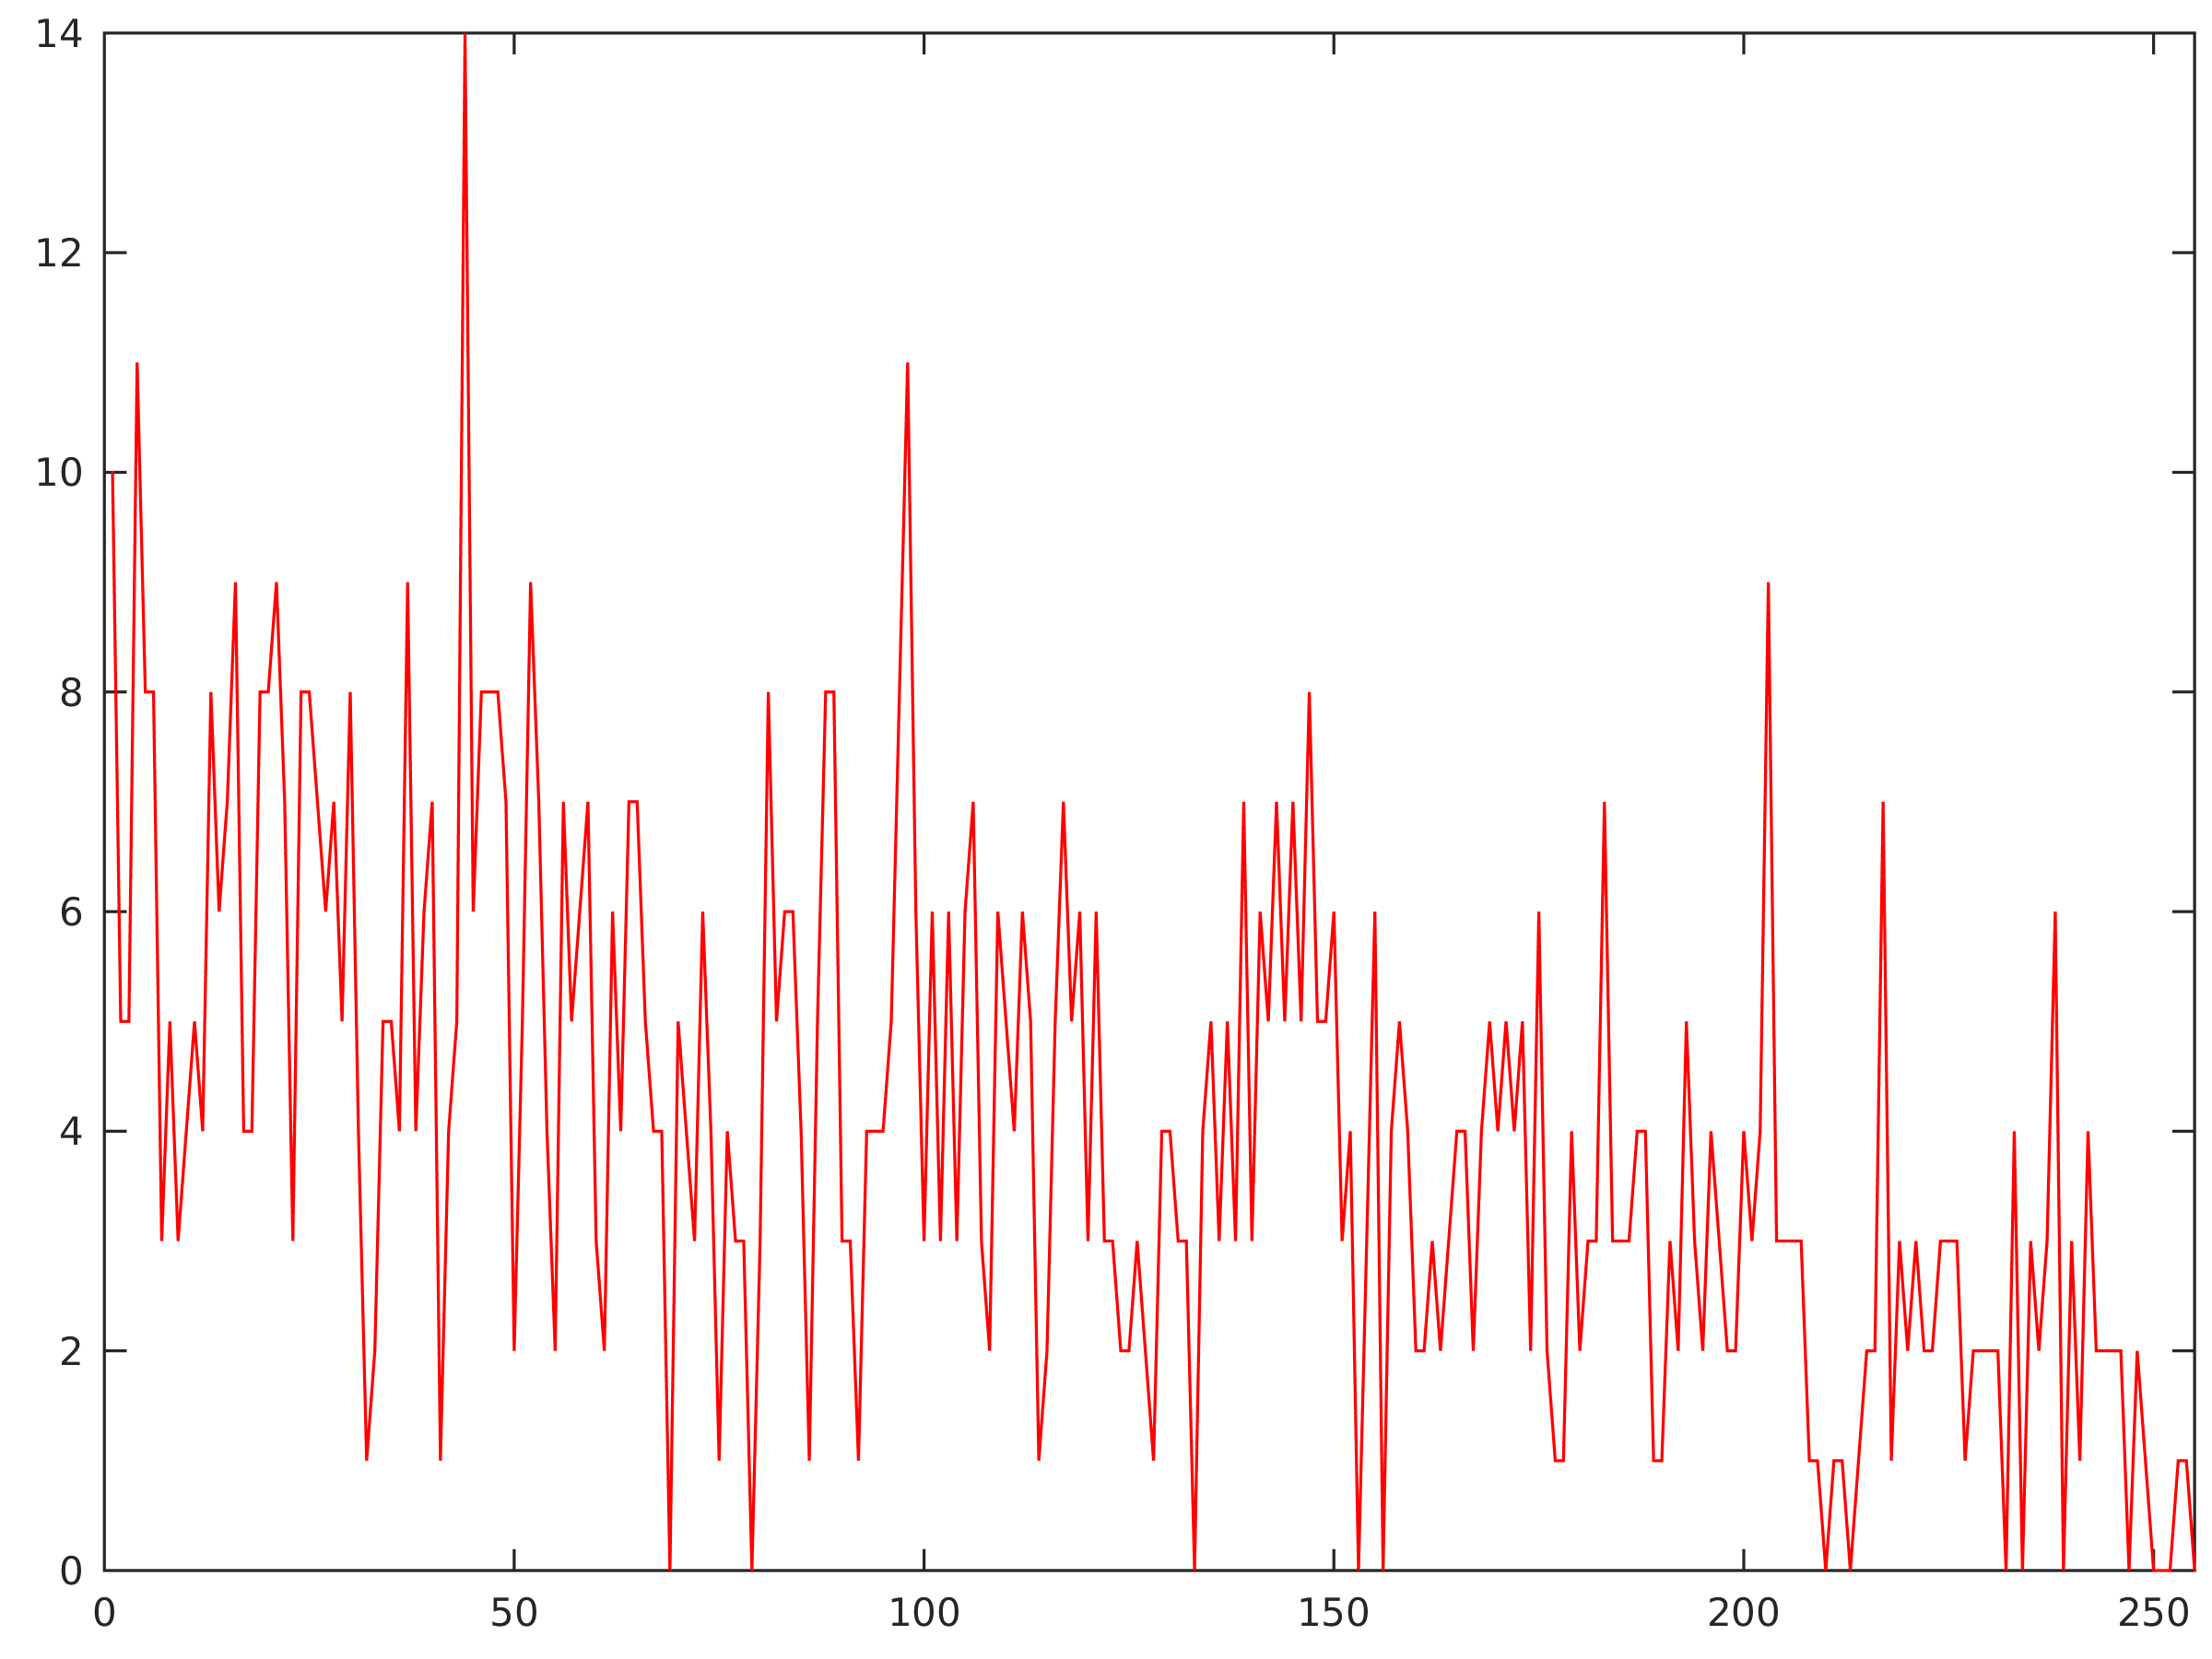
\includegraphics[width=0.25\textwidth]{0r}}
\subfigure{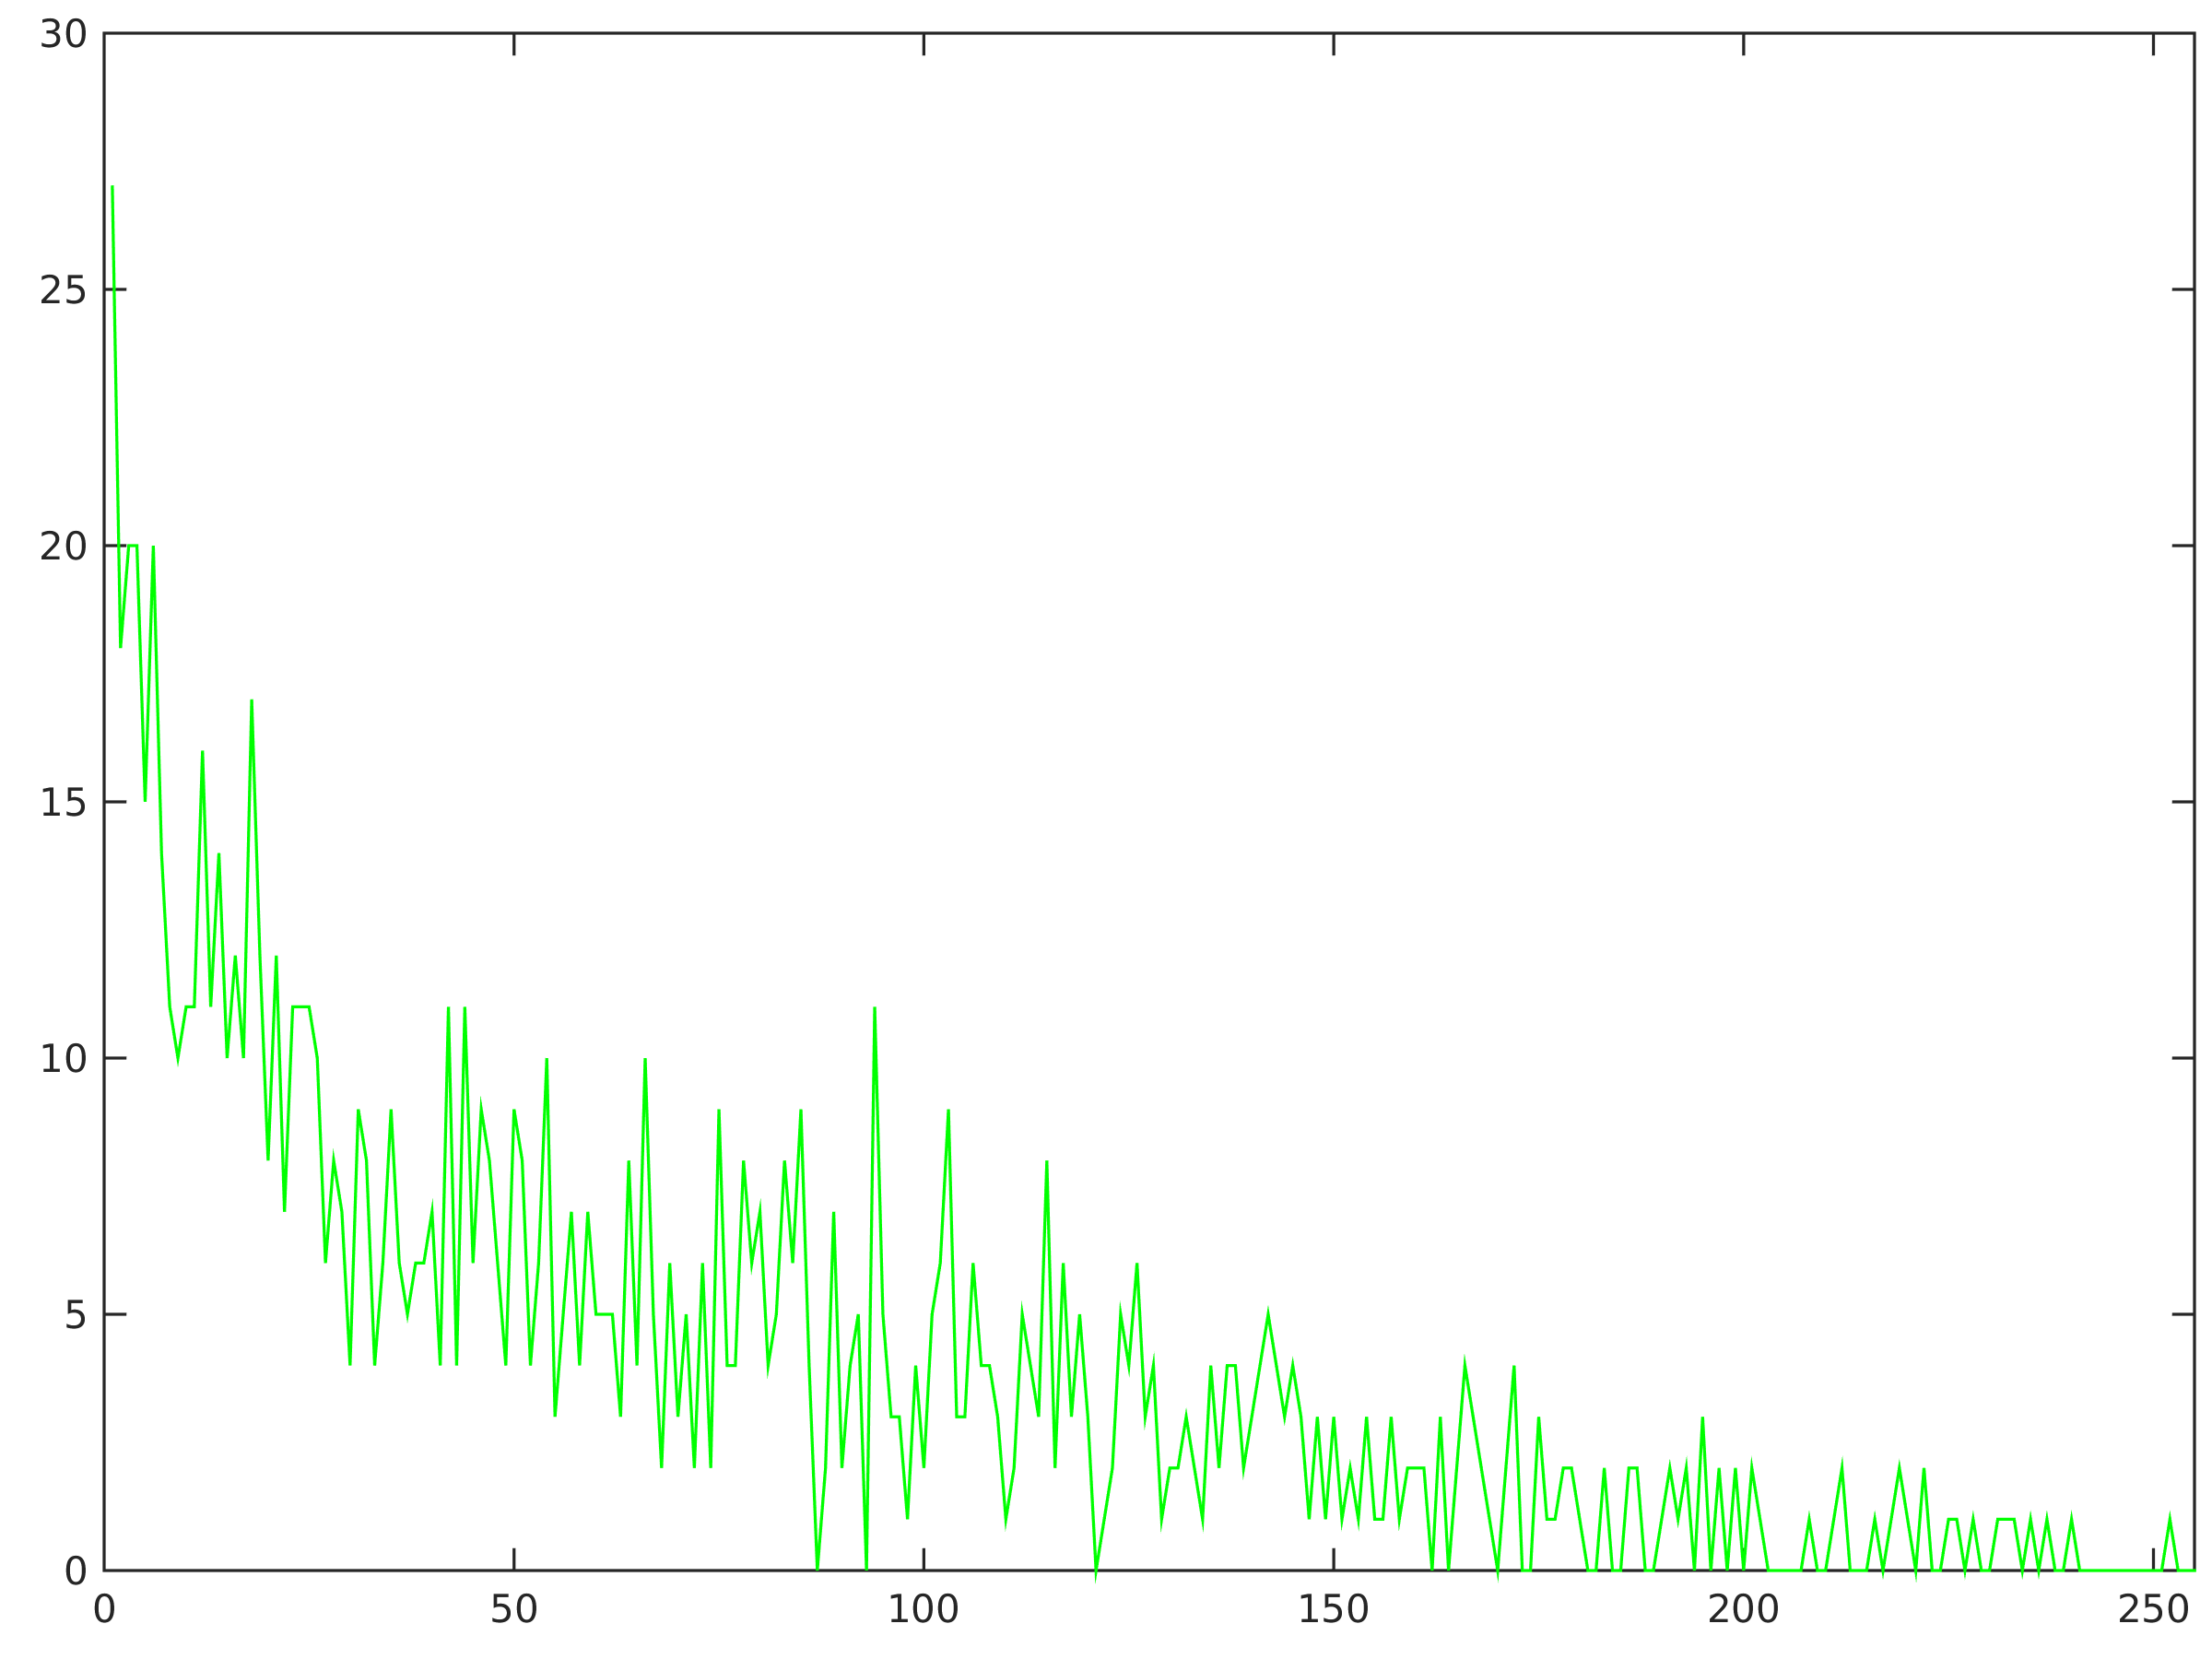
\includegraphics[width=0.25\textwidth]{0g}}
\subfigure{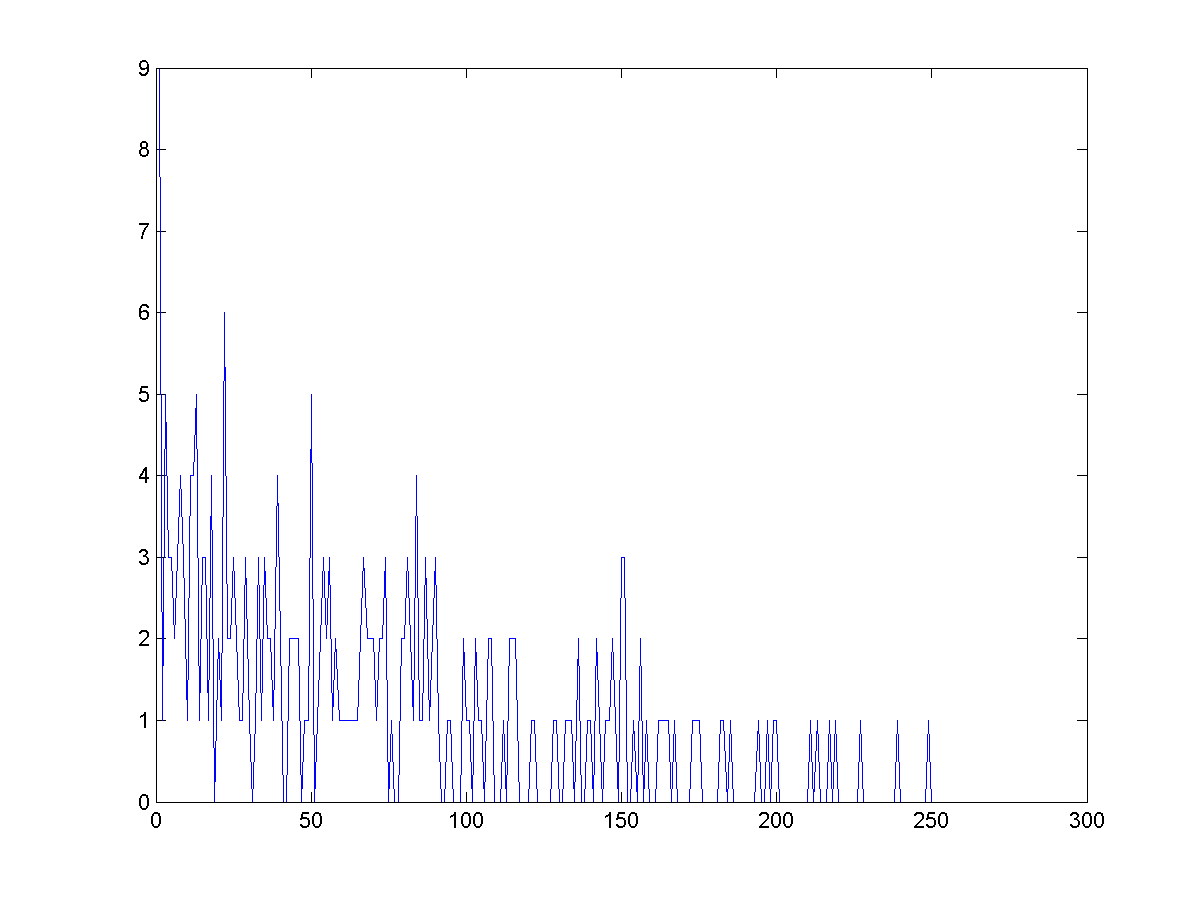
\includegraphics[width=0.25\textwidth]{0b}}
\subfigure[Label:1 1 -1]{
\includegraphics[width=0.2\textwidth]{1}}
\subfigure{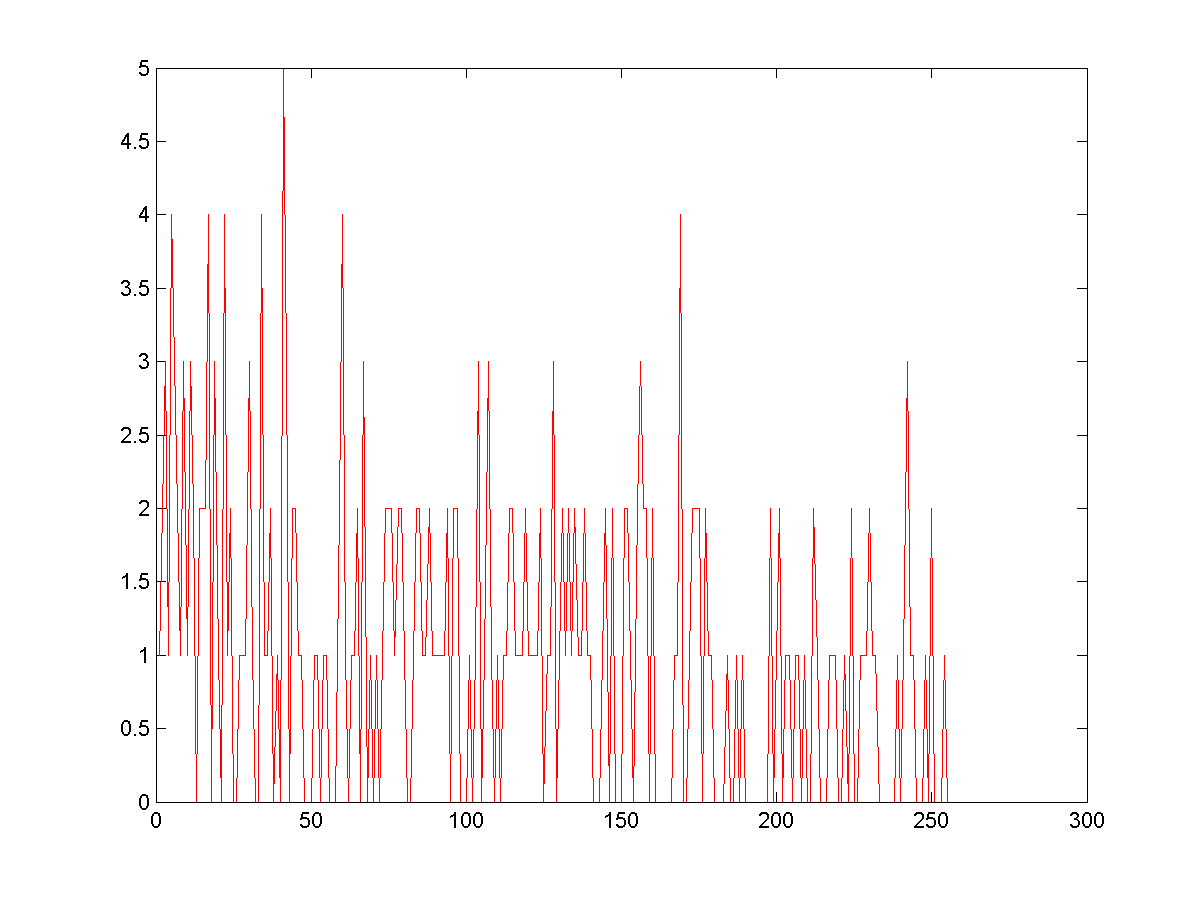
\includegraphics[width=0.25\textwidth]{1r}}
\subfigure{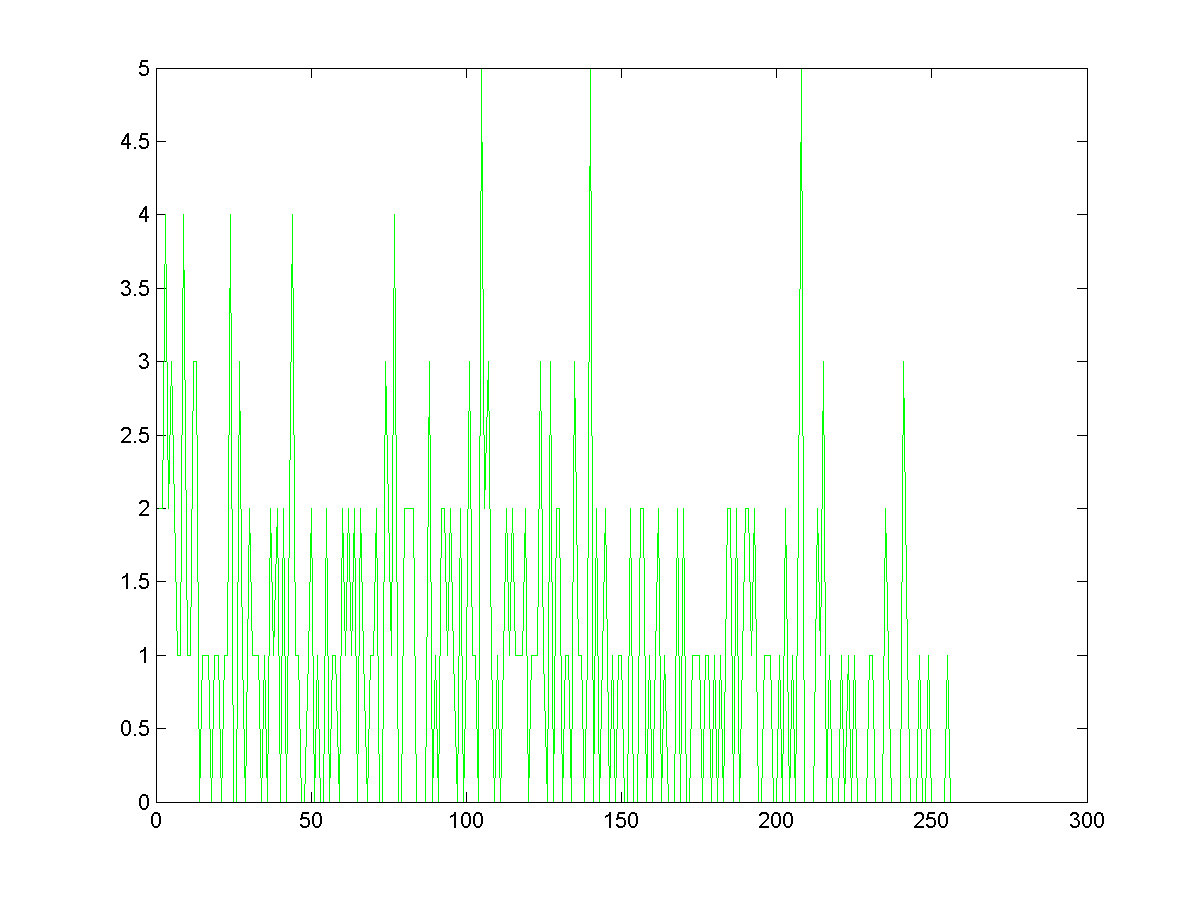
\includegraphics[width=0.25\textwidth]{1g}}
\subfigure{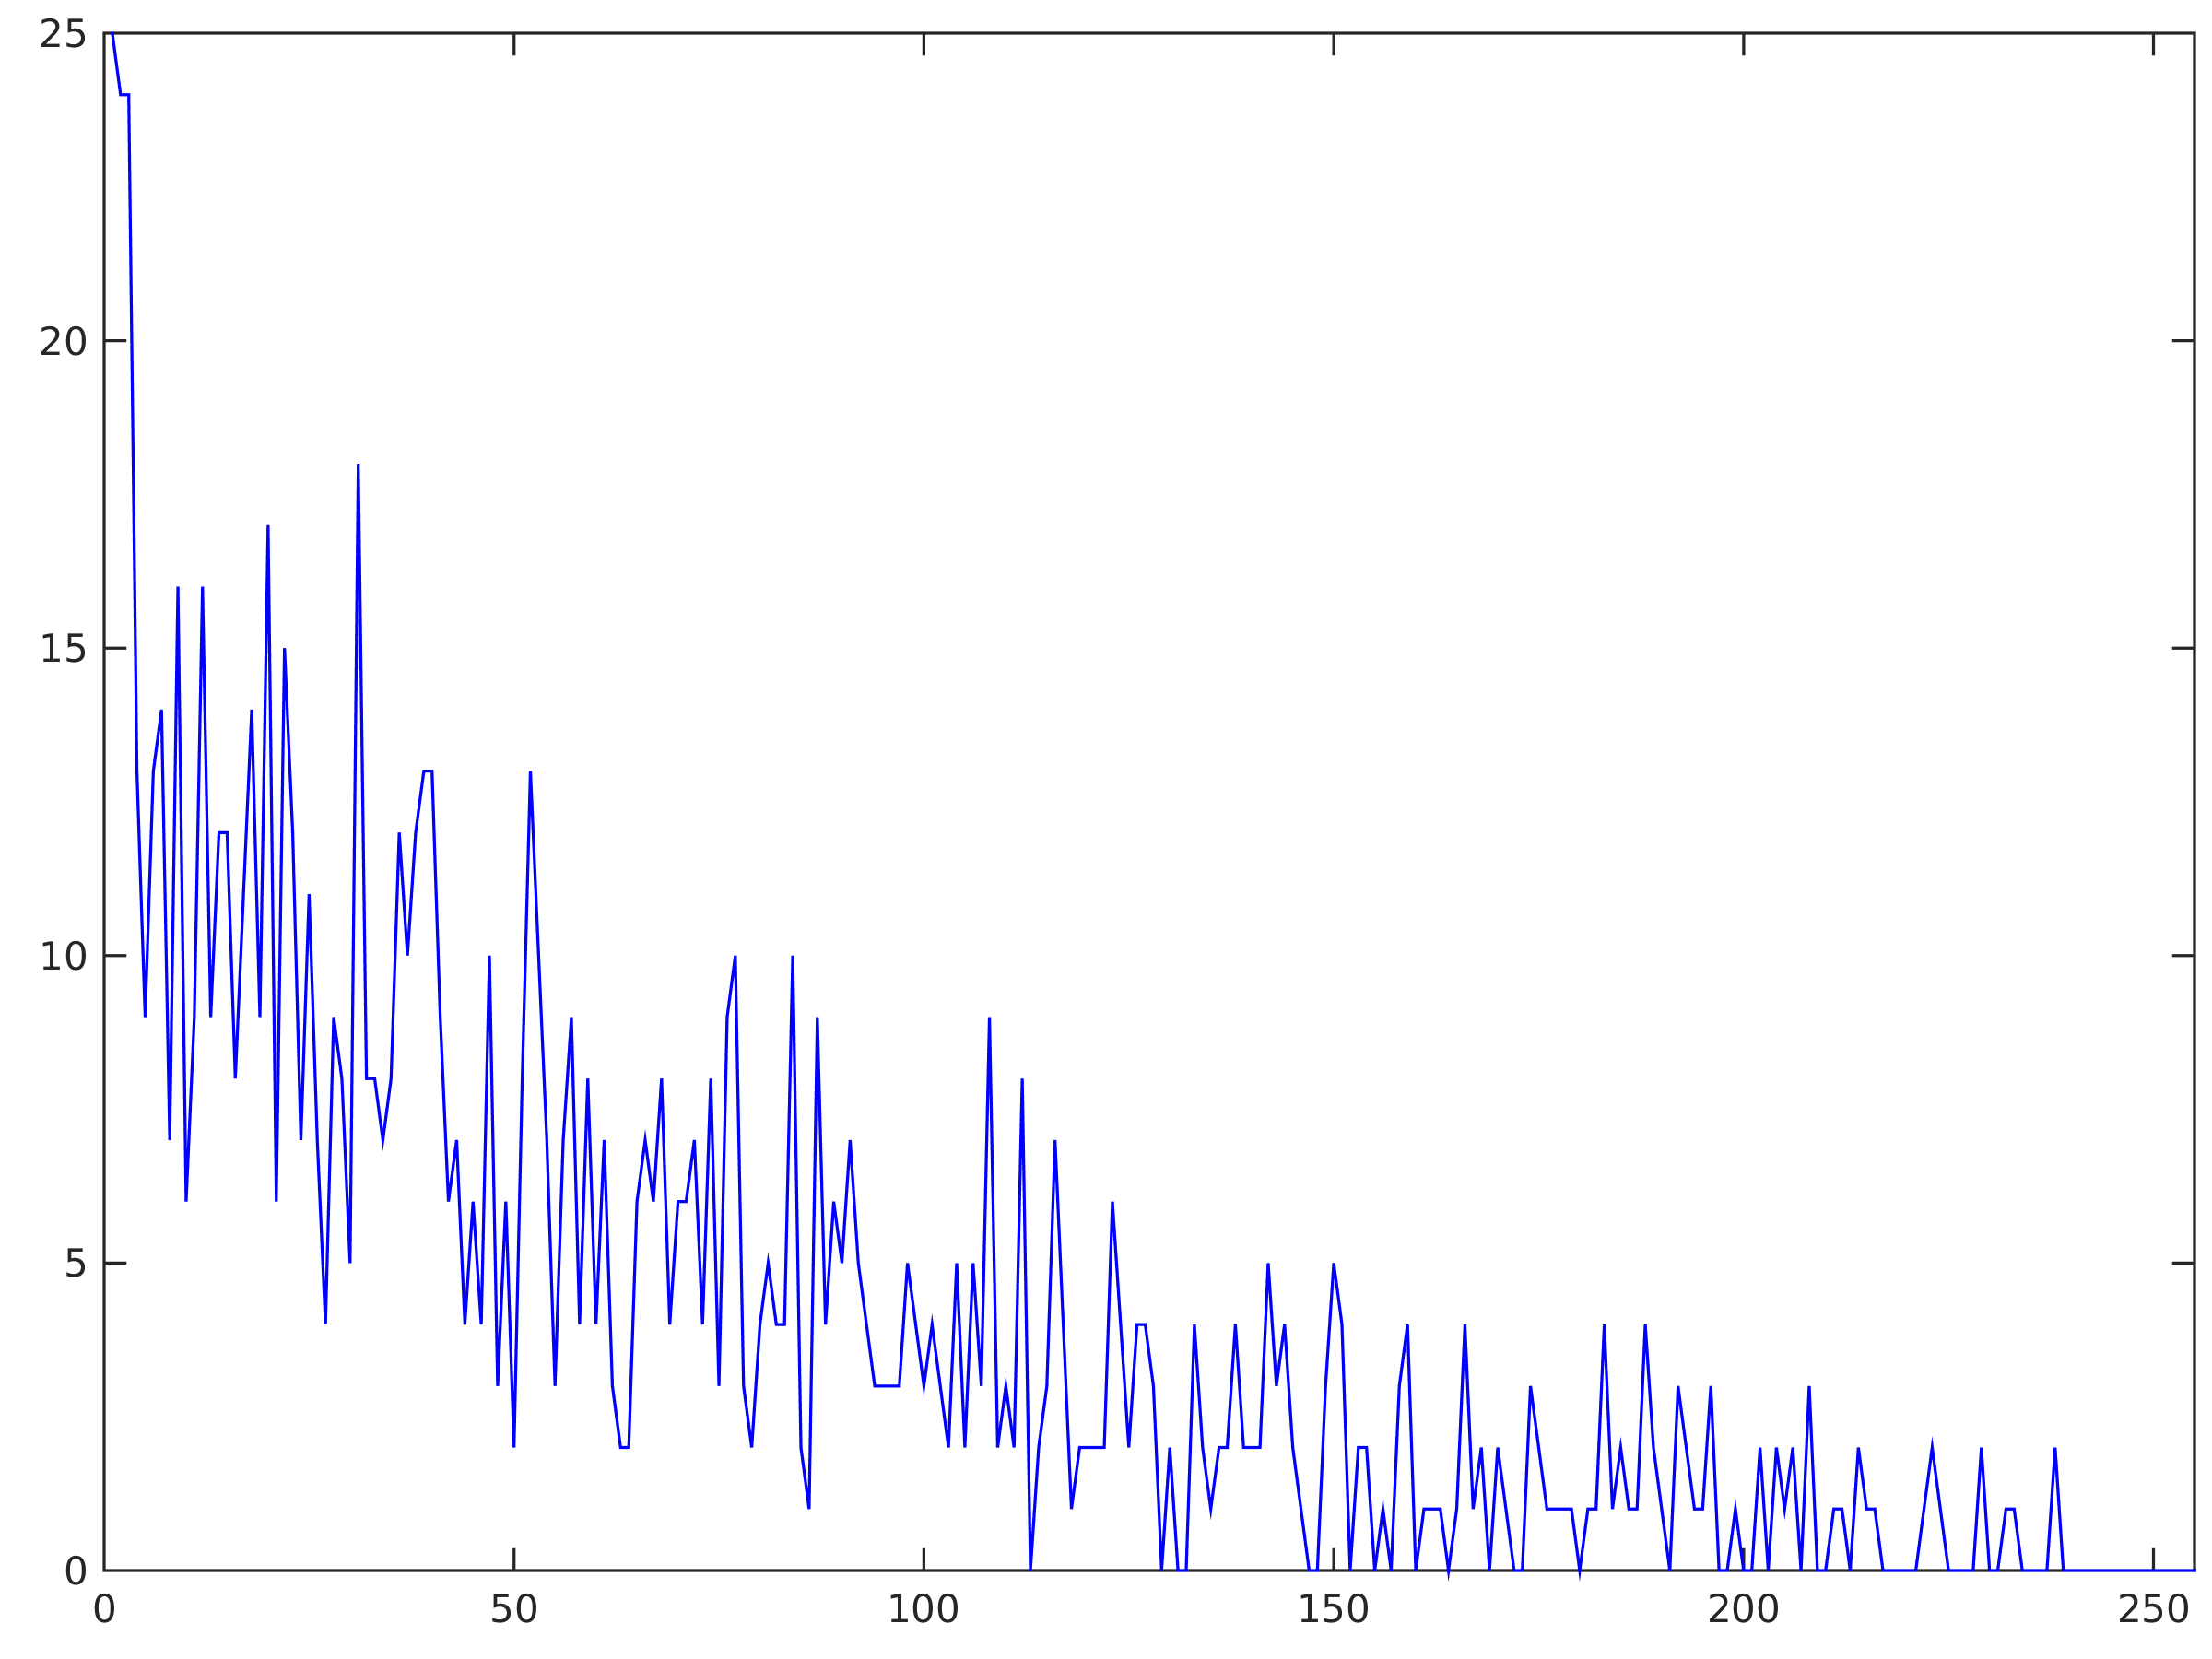
\includegraphics[width=0.25\textwidth]{1b}}
\subfigure[Label:-1 1 -1]{
\includegraphics[width=0.2\textwidth]{2}}
\subfigure{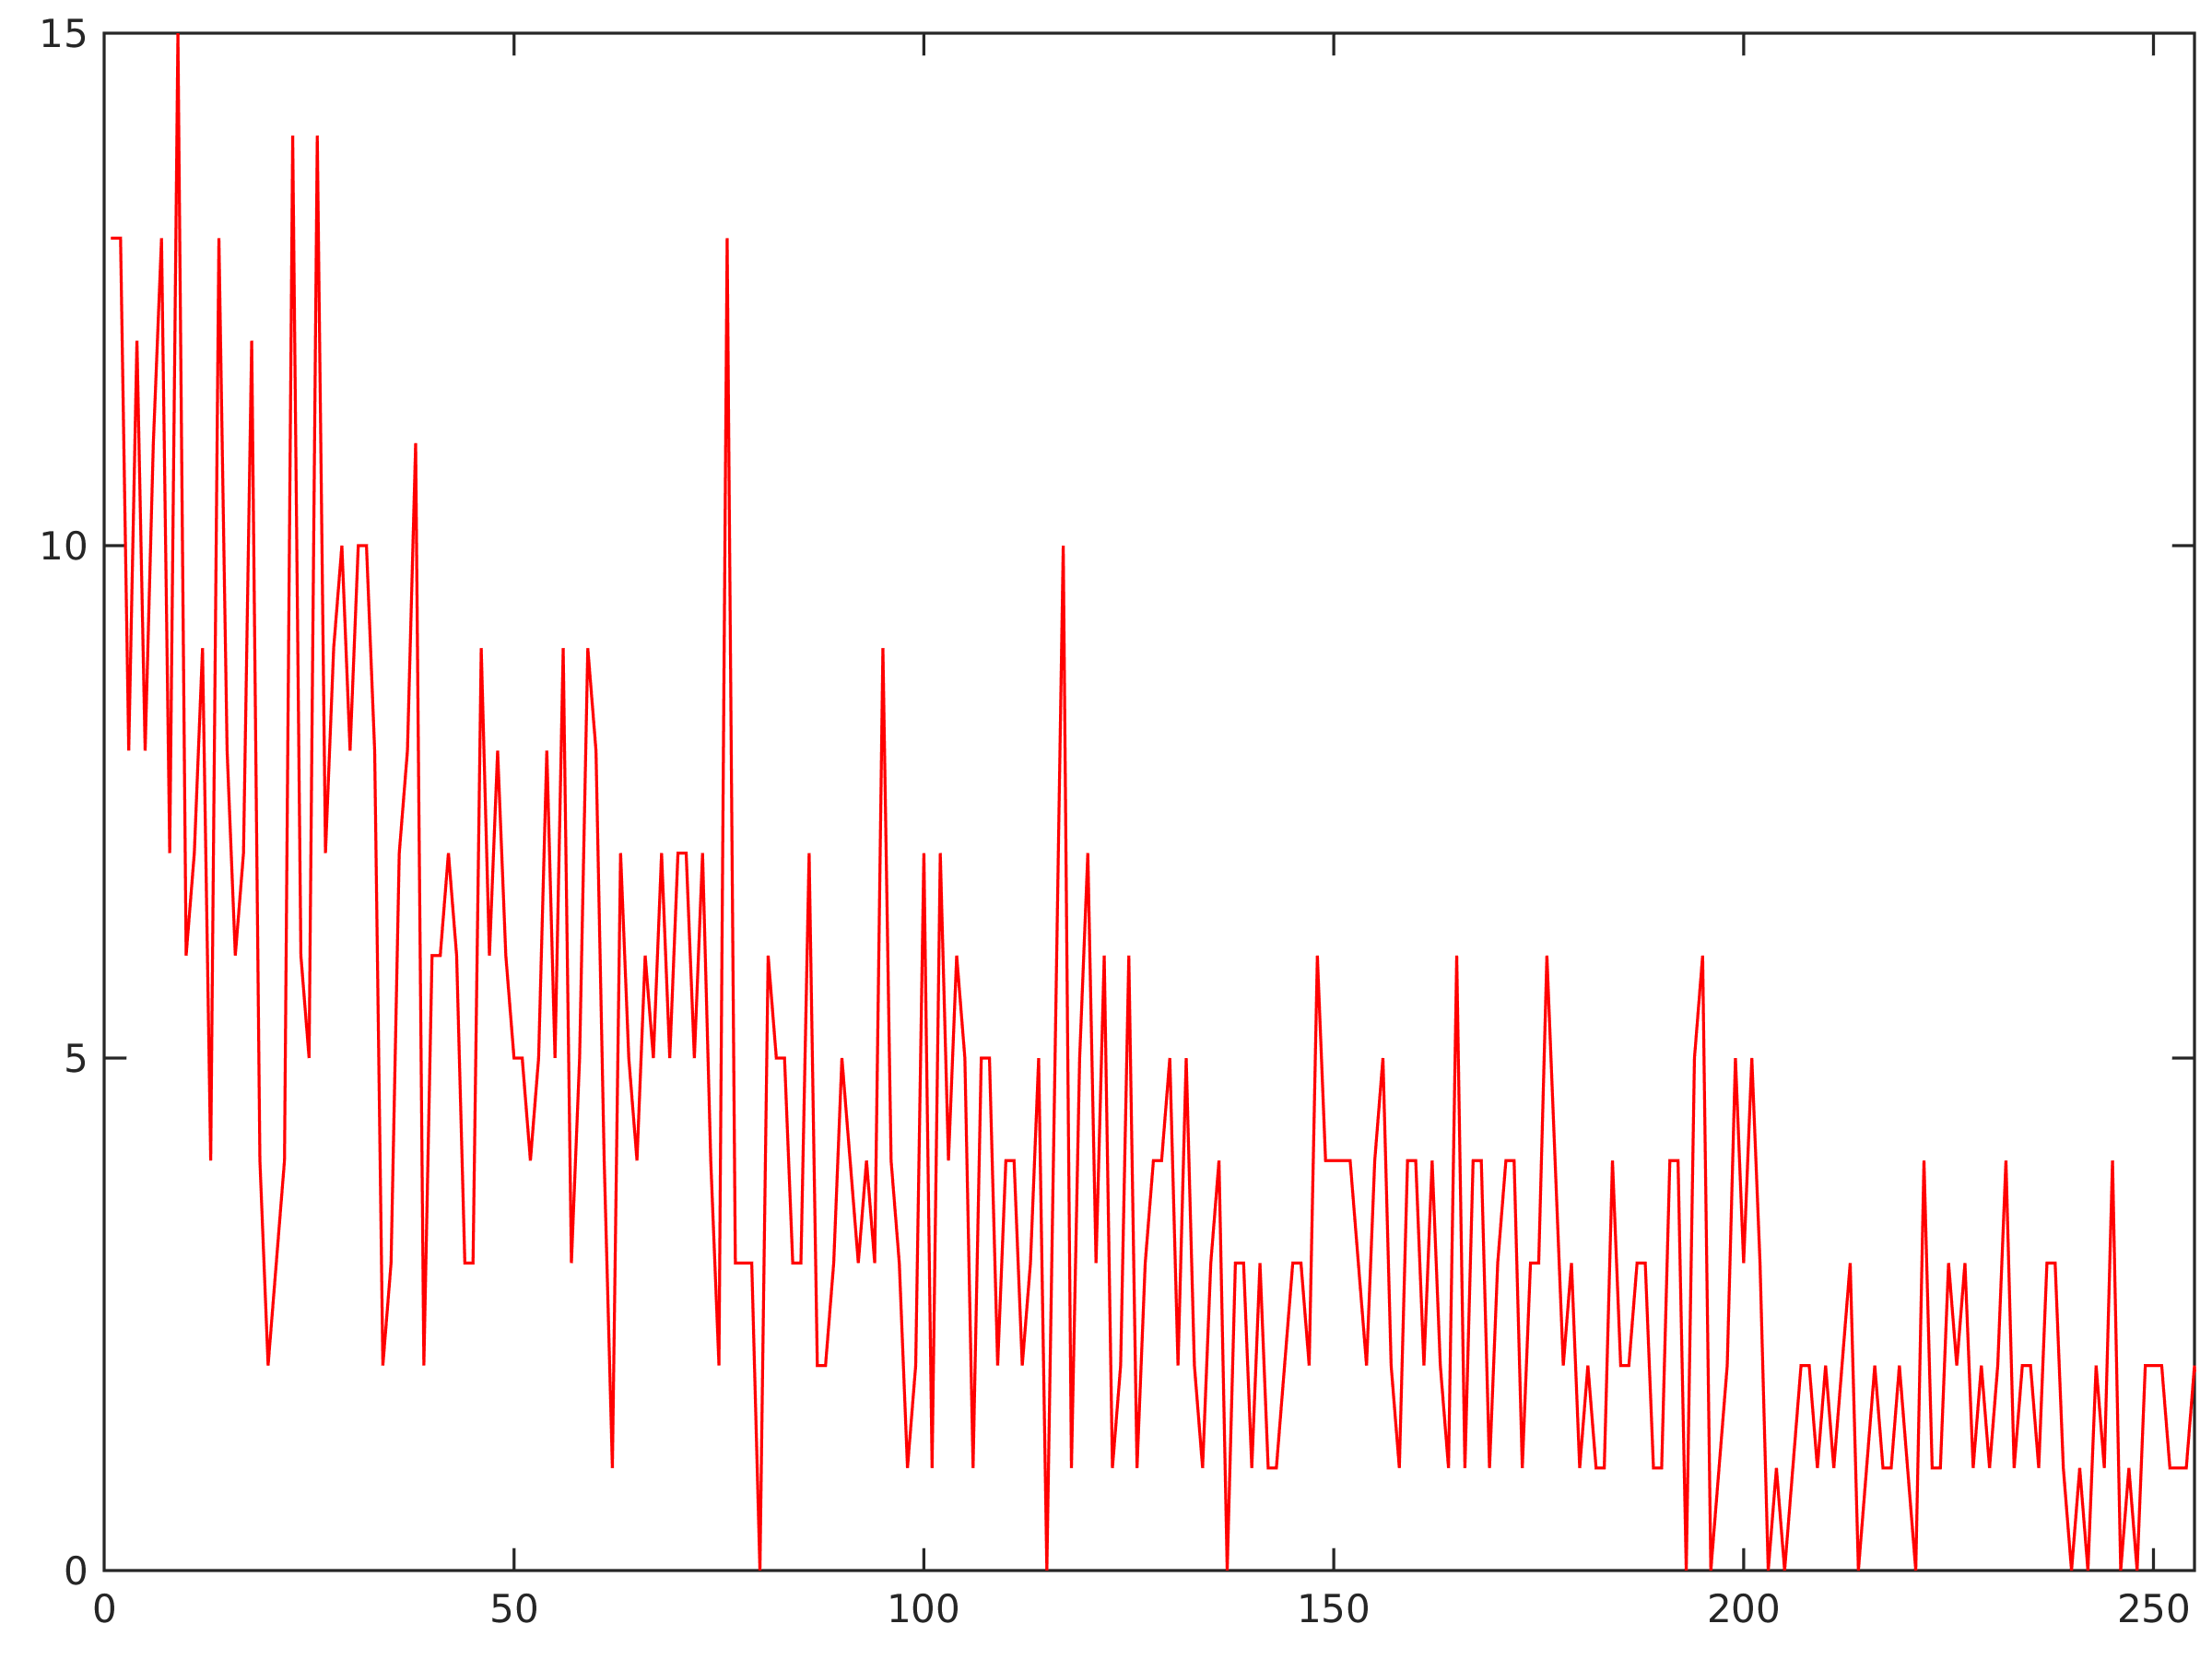
\includegraphics[width=0.25\textwidth]{2r}}
\subfigure{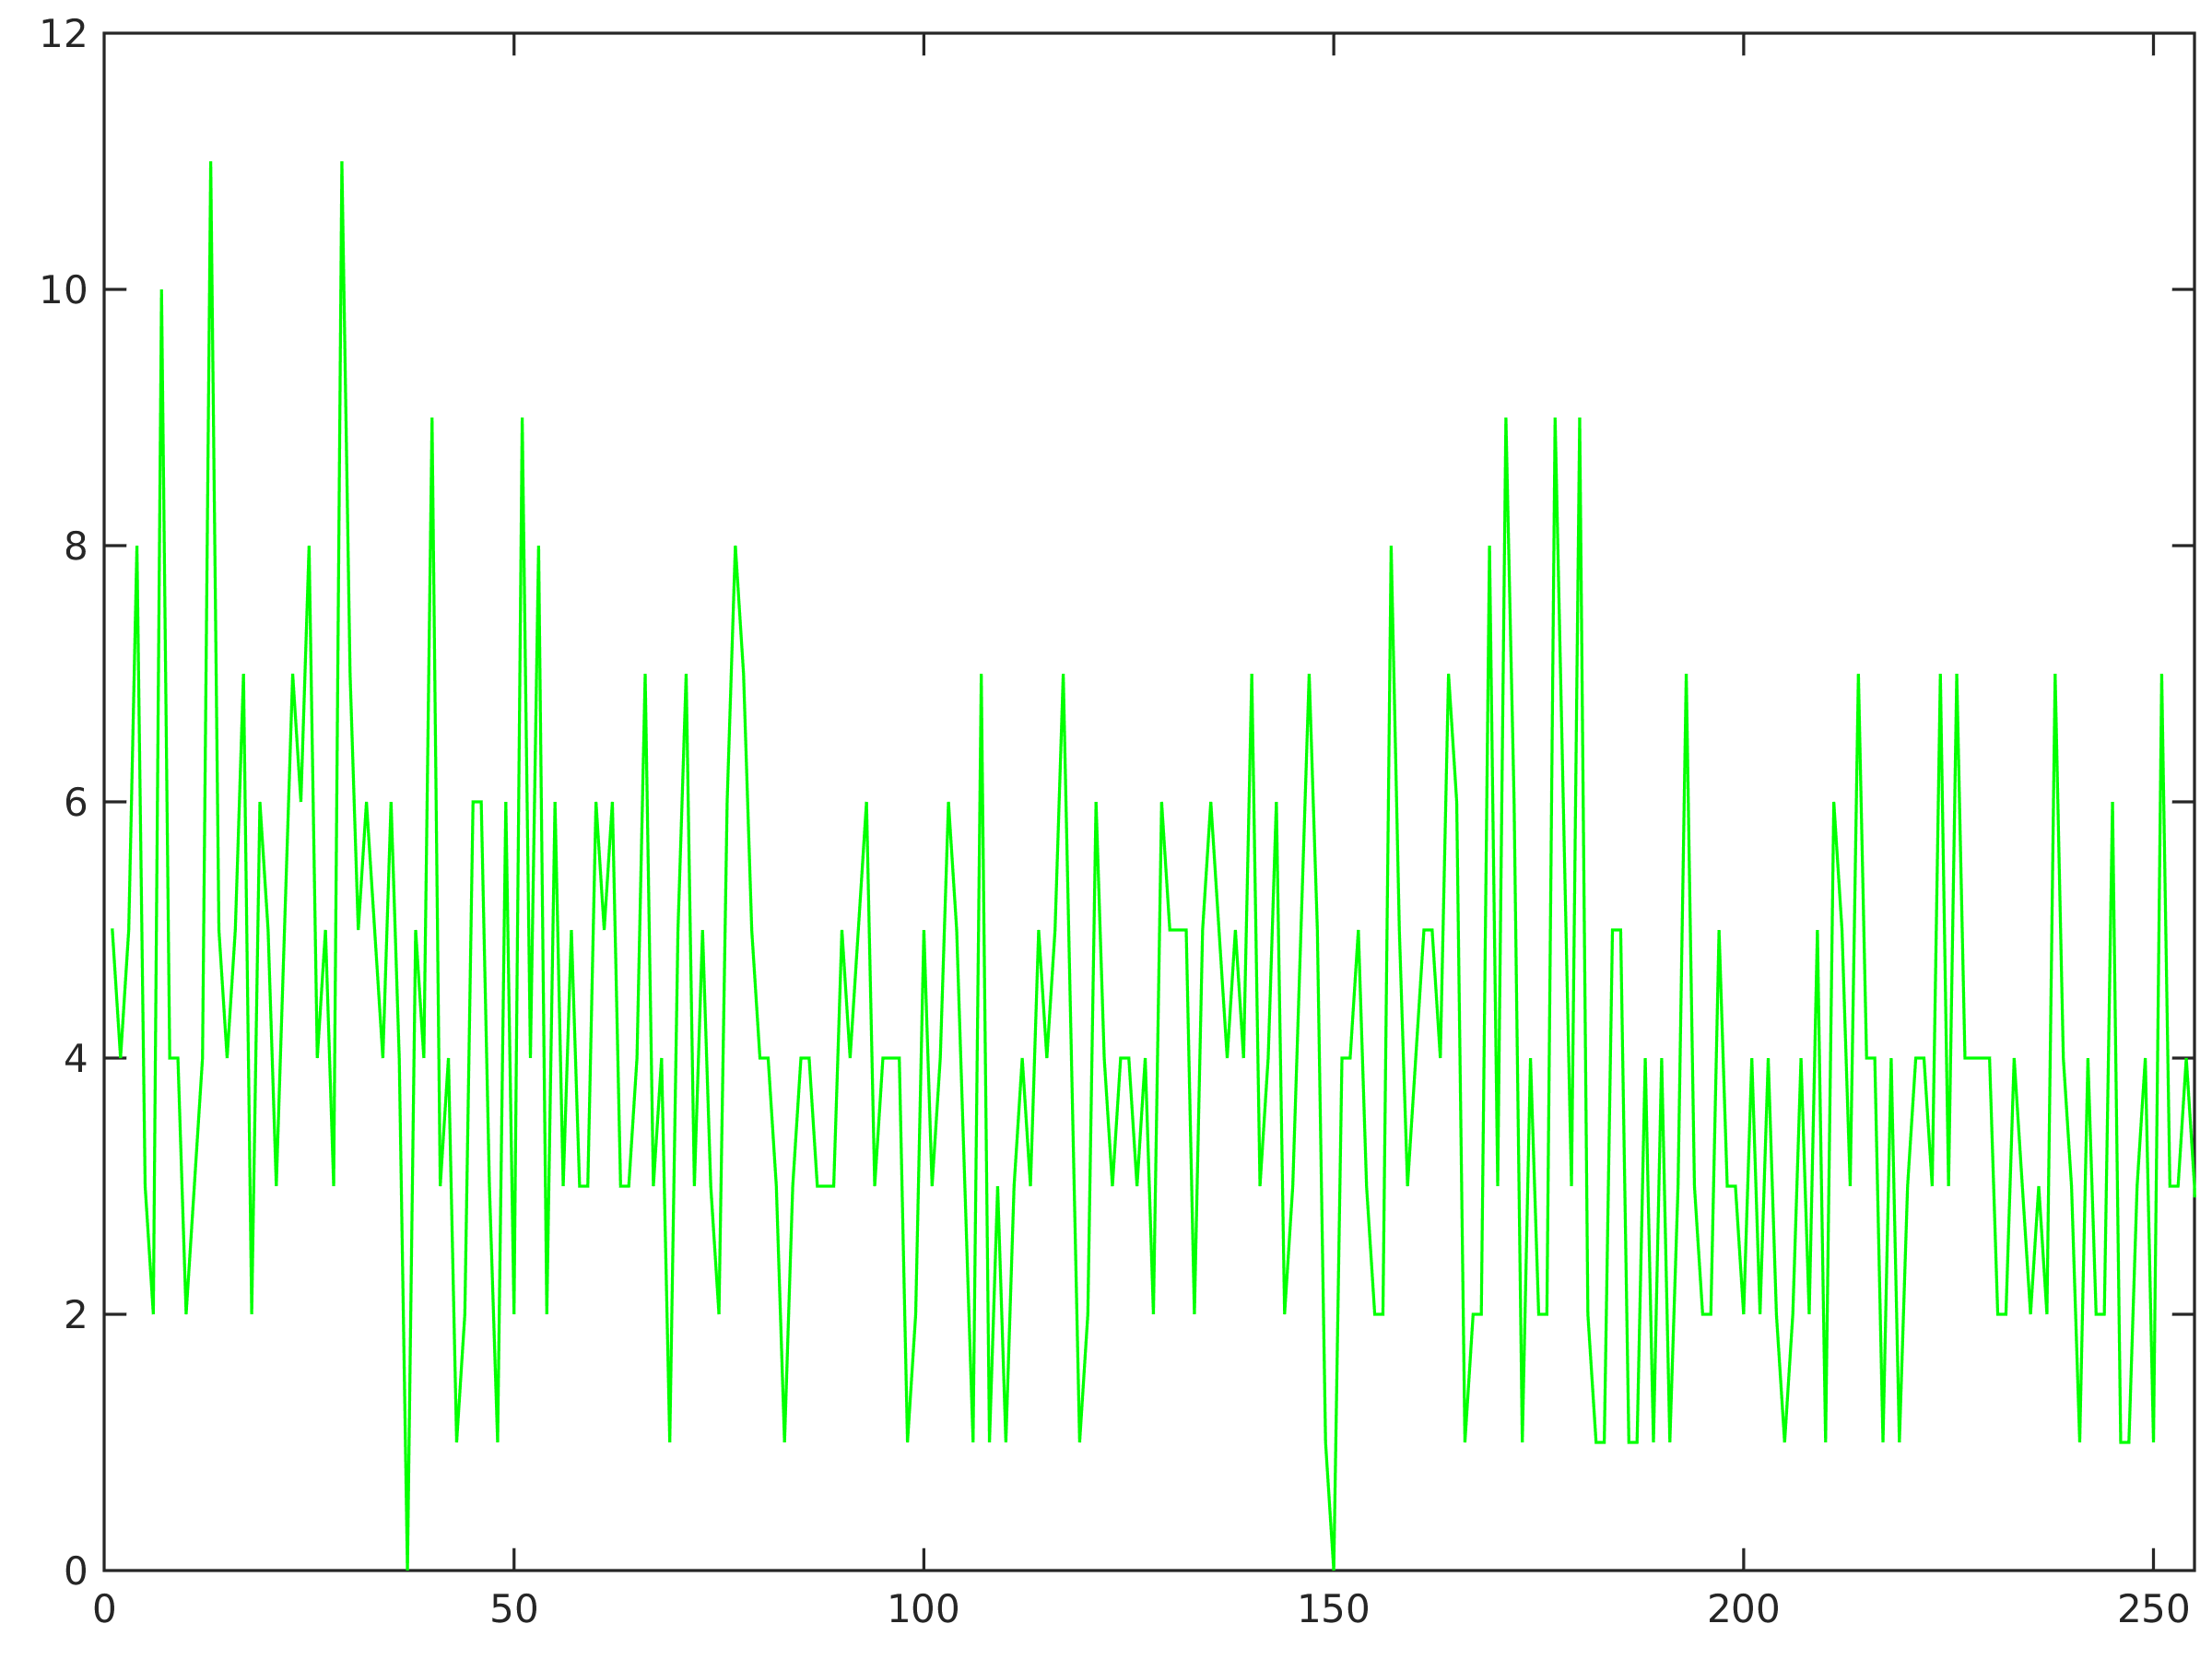
\includegraphics[width=0.25\textwidth]{2g}}
\subfigure{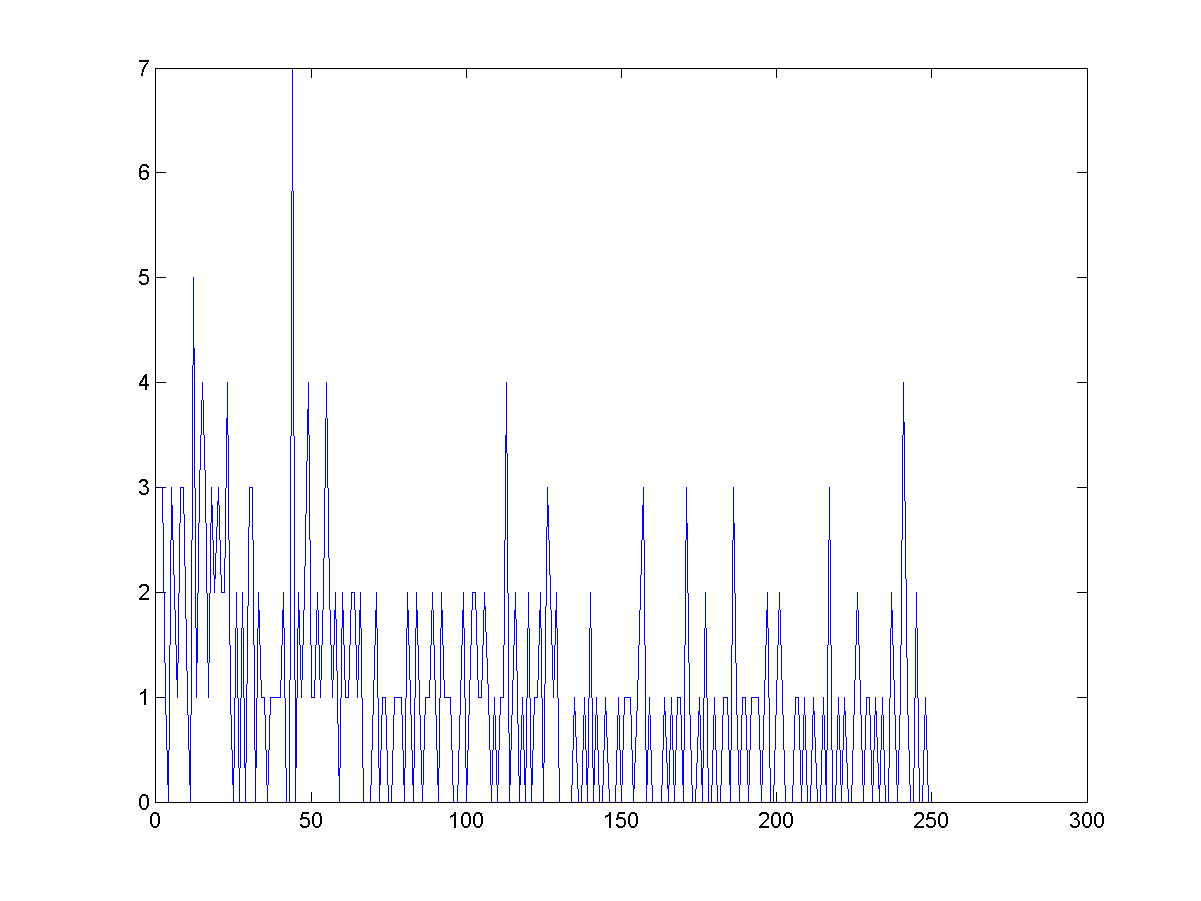
\includegraphics[width=0.25\textwidth]{2b}}
\subfigure[Label:-1 -1 1]{
\includegraphics[width=0.2\textwidth]{3}}
\subfigure{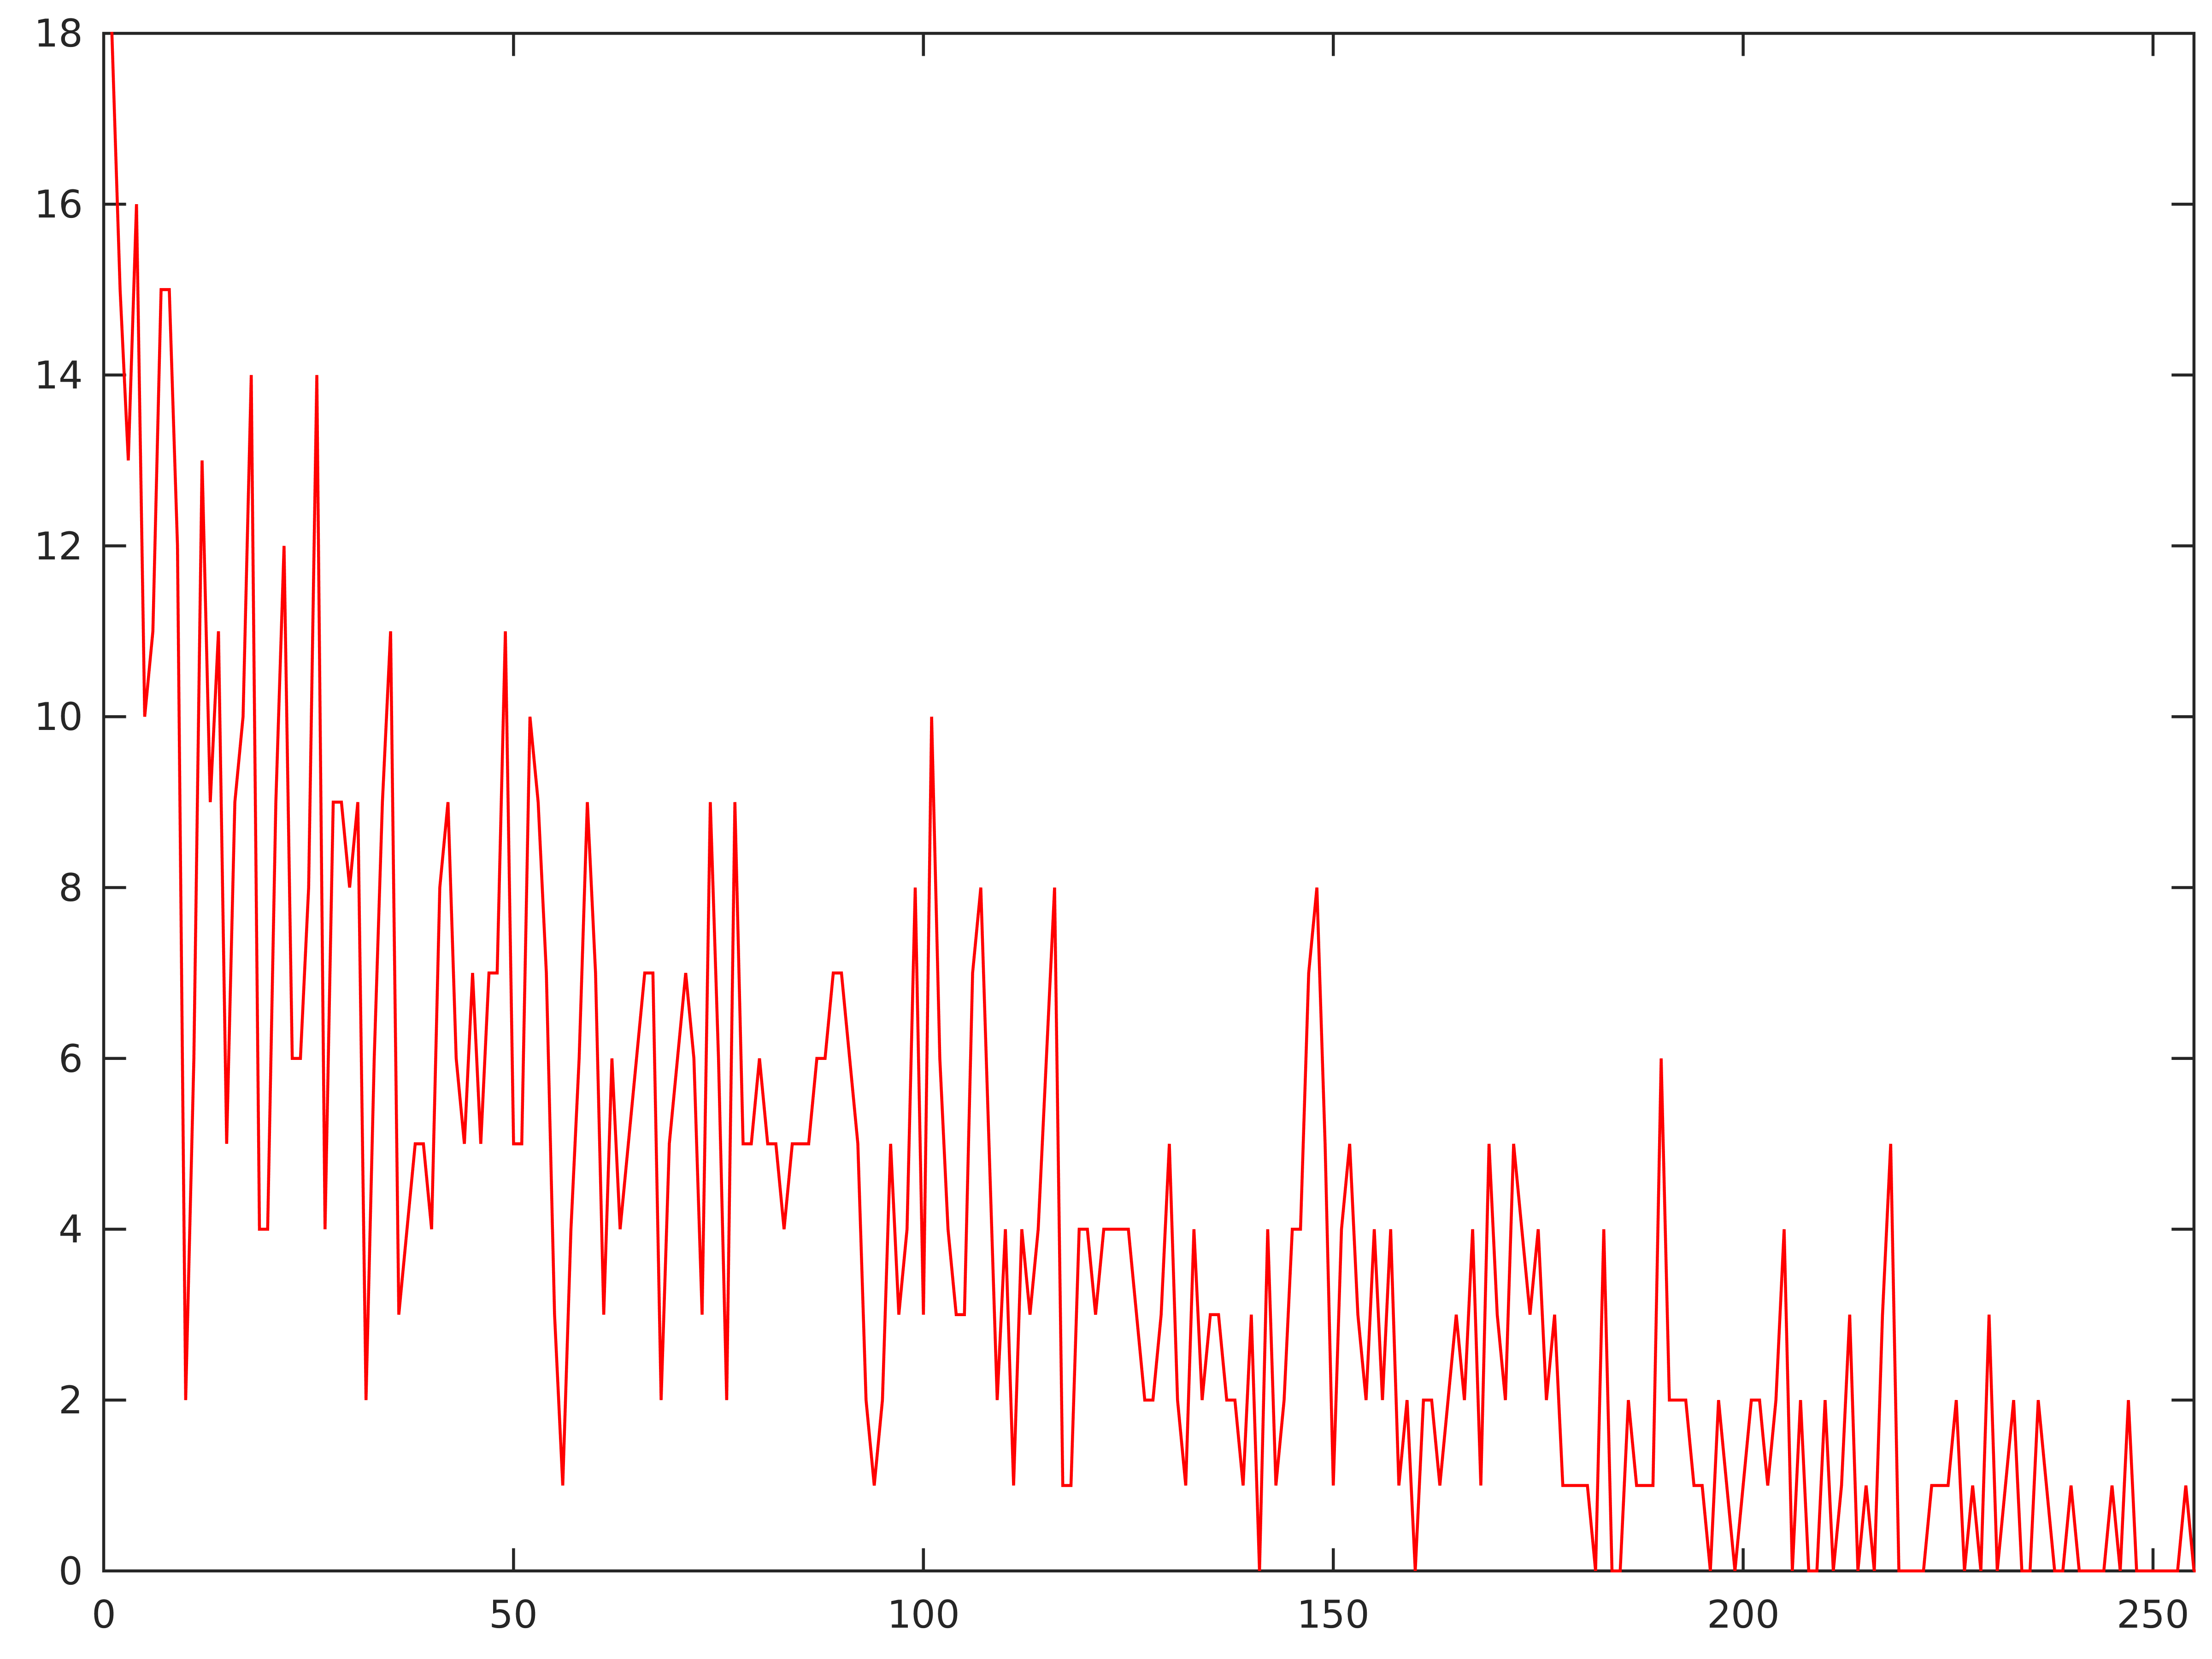
\includegraphics[width=0.25\textwidth]{3r}}
\subfigure{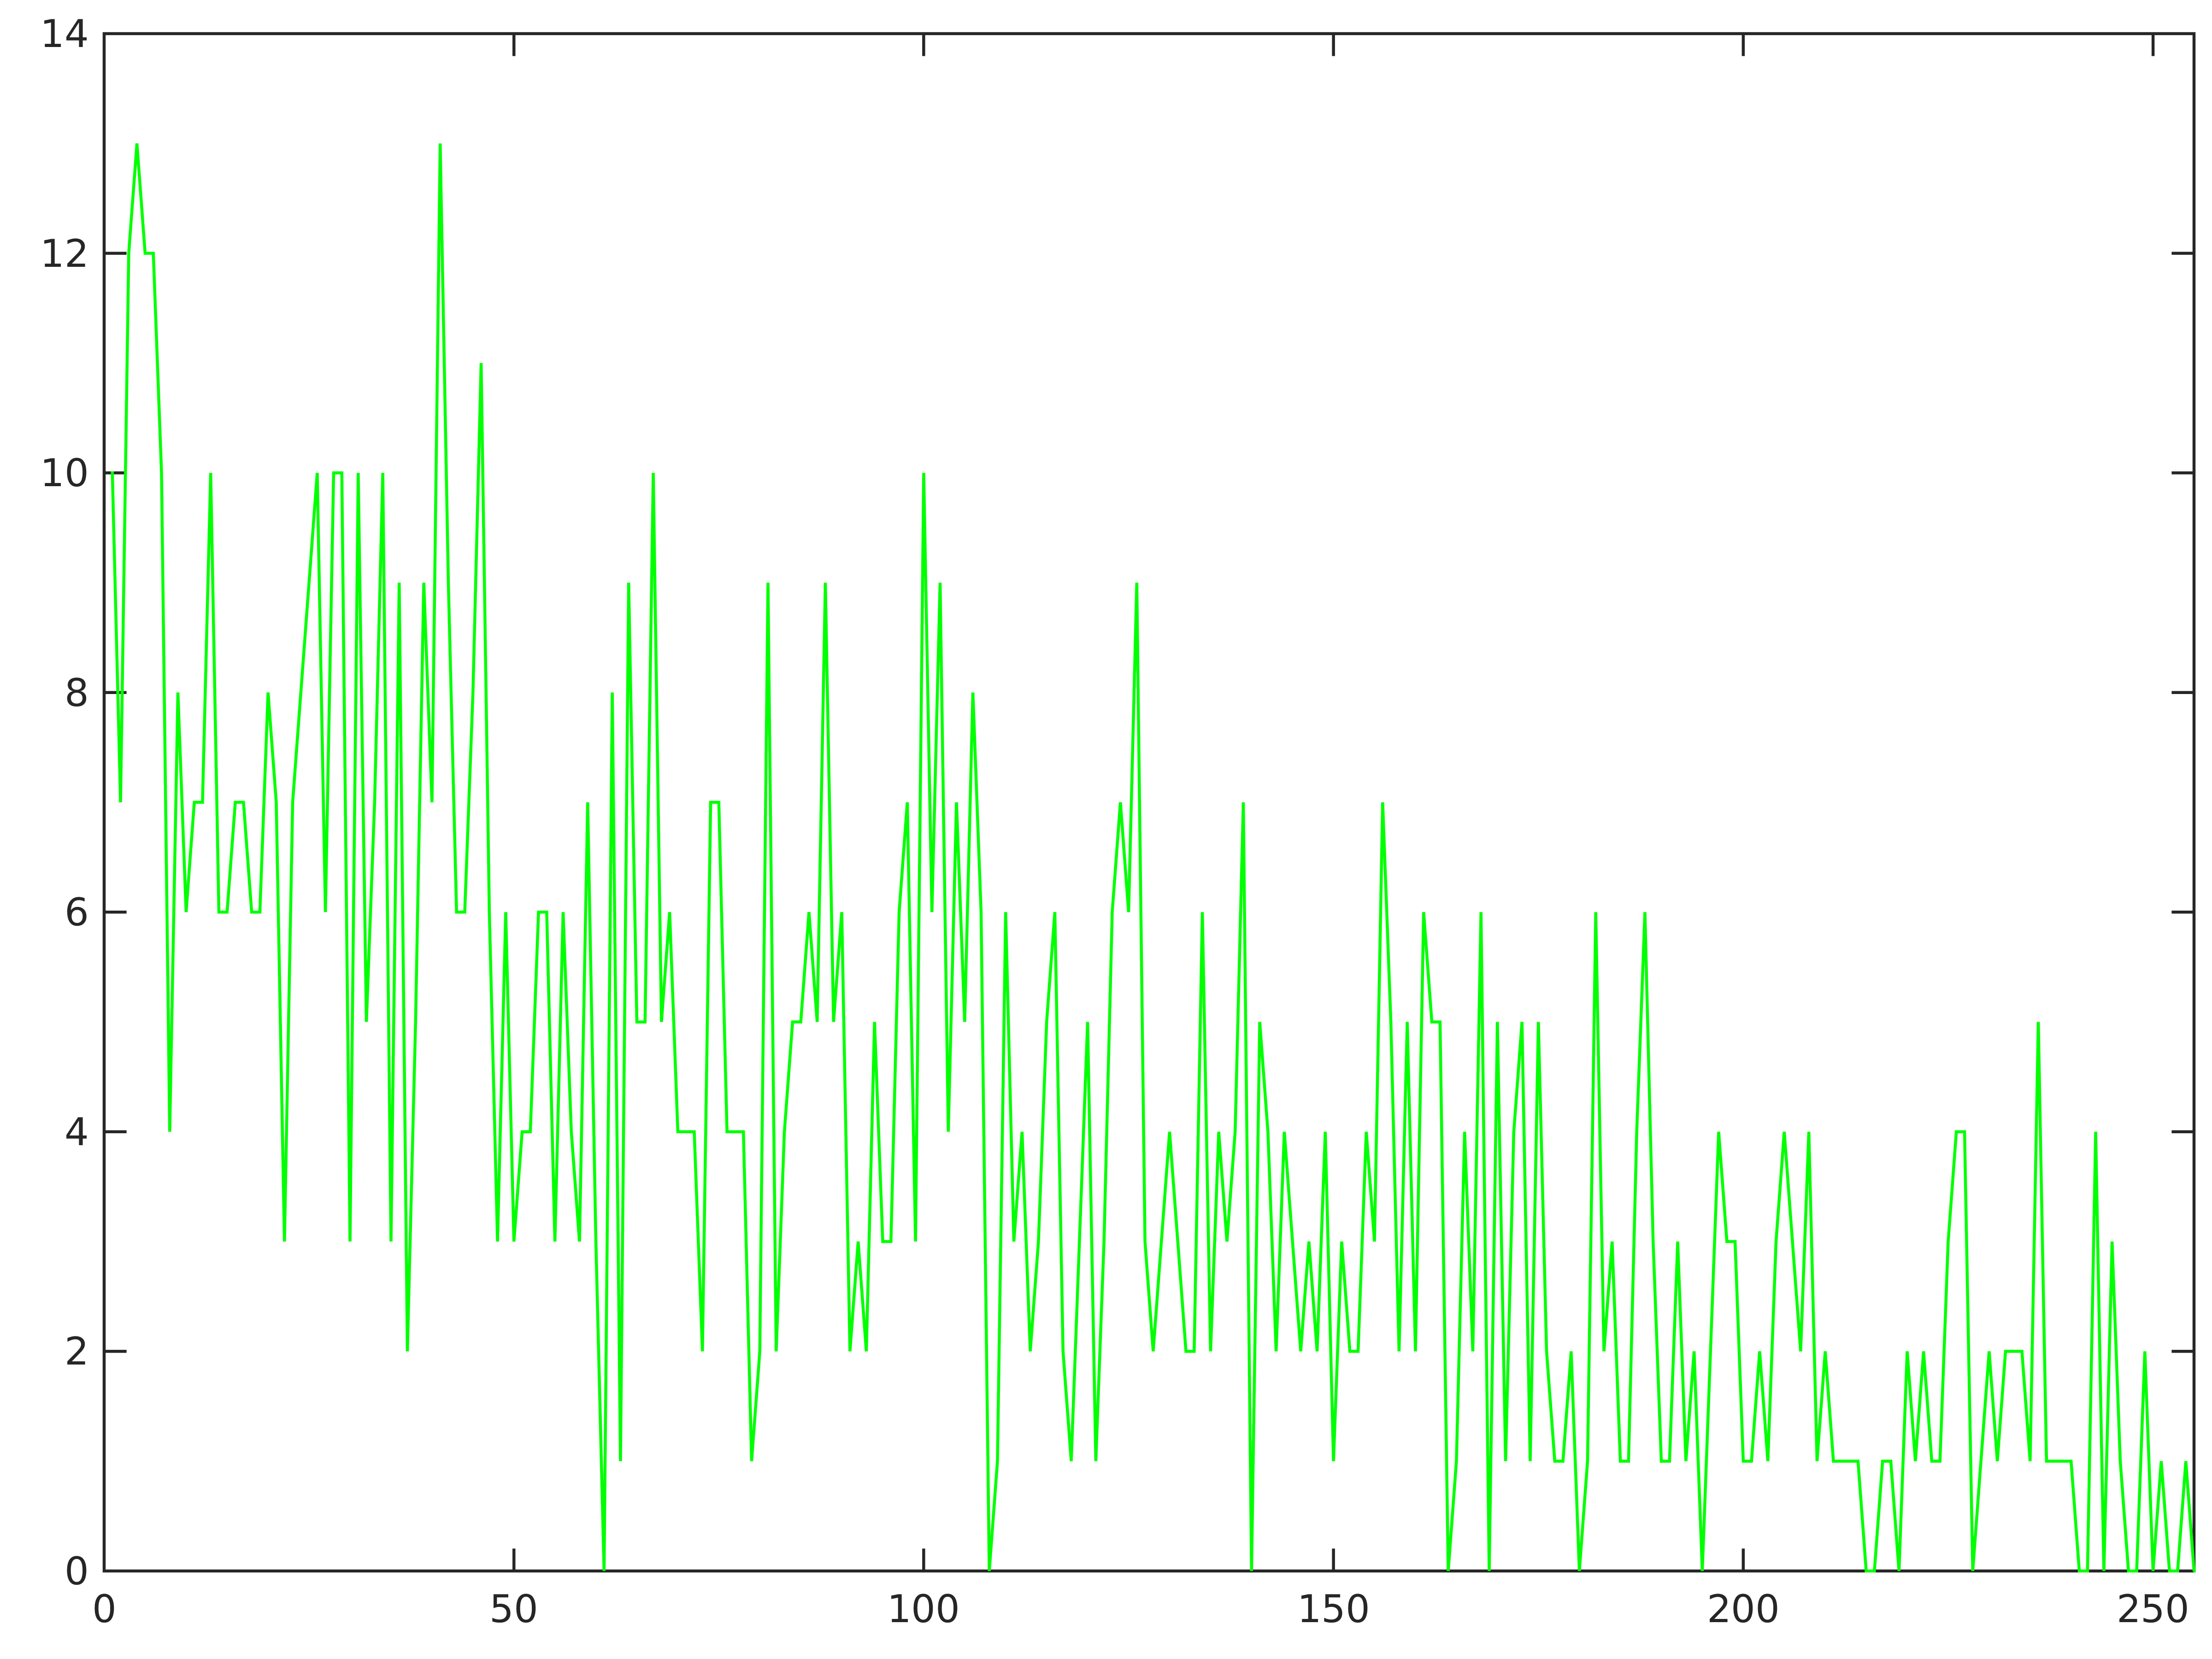
\includegraphics[width=0.25\textwidth]{3g}}
\subfigure{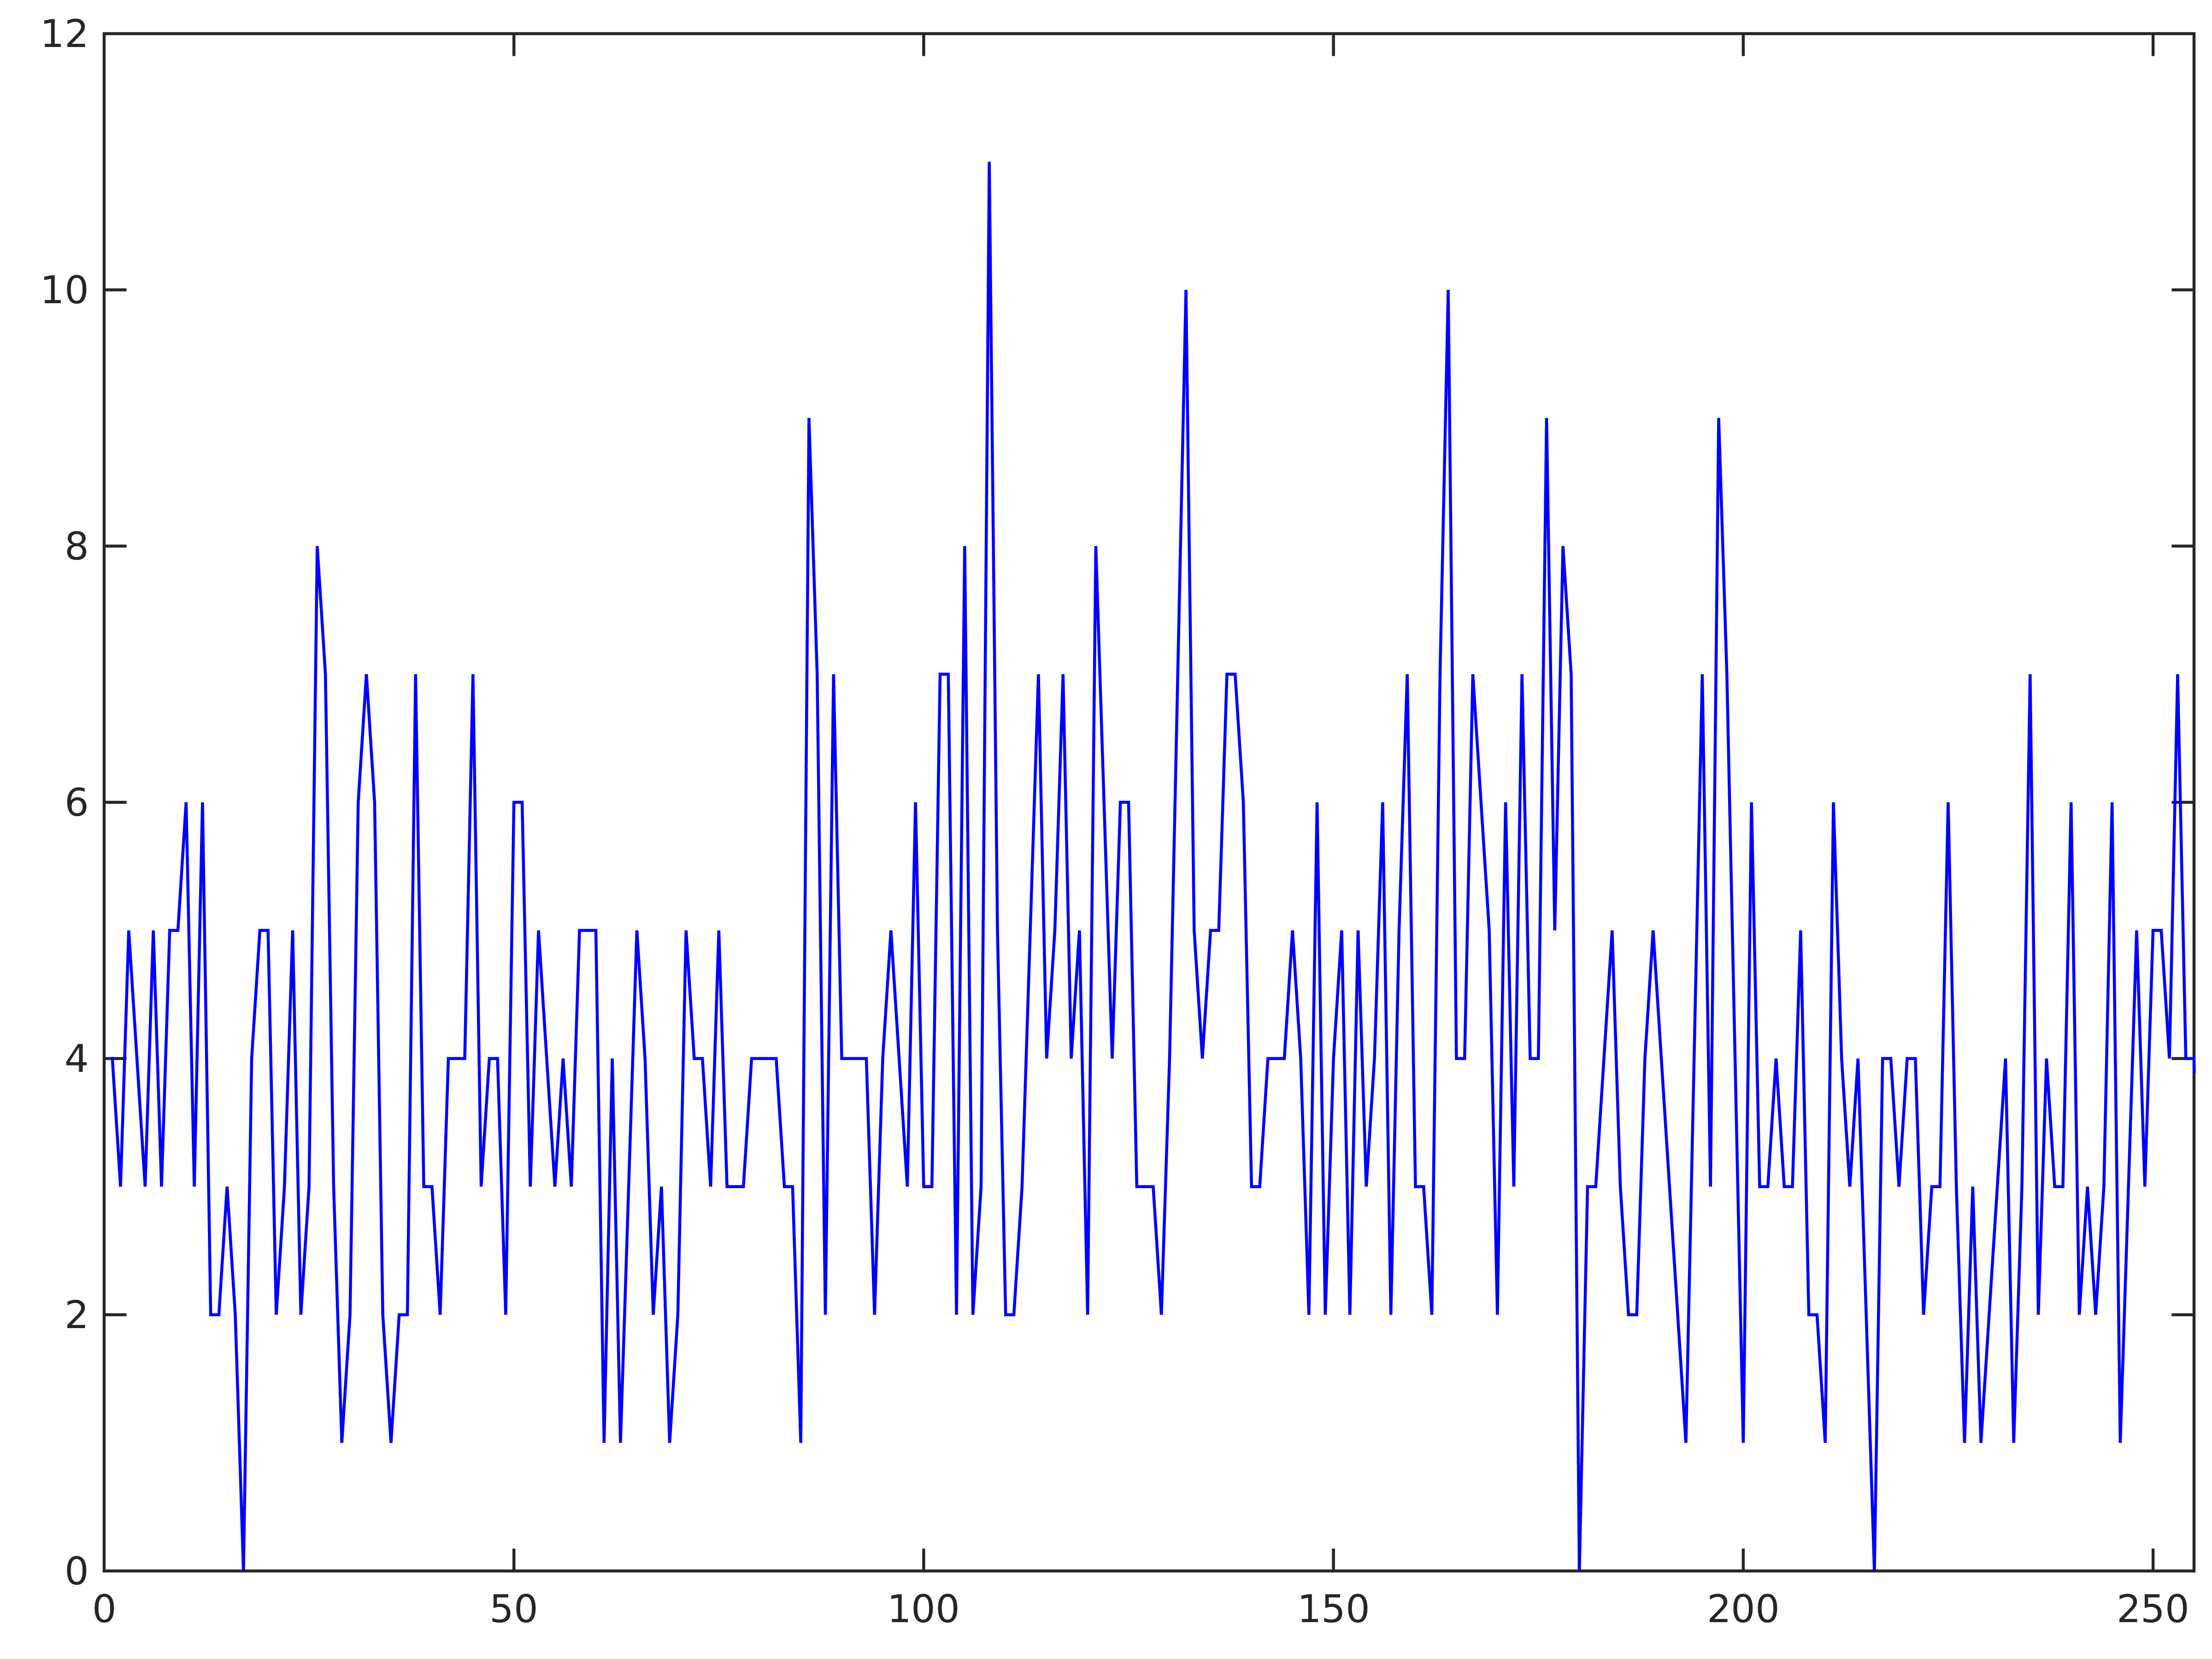
\includegraphics[width=0.25\textwidth]{3b}}
\caption{Multilabel samples and the RGB colour histograms. Three labels mean red, green and blue sequentially. }
\end{figure}

The dataset contains $1000$ images in total. $960$ images are training samples and $40$ are test samples. 

\section{Artificial Neural Network}

The Artificial Neural network is an approach to learning a nonlinear function which can be used to map samples to multi labels. The neurons in the first layer take a raw image while the neurons in the last layer produce outputs. Between the first and the last layers, the middle layers are called hidden layers because they do not connect to external world. A 3 layer neural network can represent any bounded degree polynomial under certain conditions\citep{barron1993universal}. The weights of neural network are learned by algorithms deployed over training dataset. One of successful learning algorithms is the Backpropagation algorithm which updates weights by propagating errors caused by comparing prediction for each sample with actual target values.

Two factors will be modified to adapt a neural network to do multi-label classification. One is to design a new error function which fits the characteristics of multi-label samples instead of single-label ones. The other is to find a moderate metric according to the new designed error function.

\subsection{Network Architecture}

Define $\mathcal{X} = \mathbb{R}^{d}$ as the sample space and $\mathcal{Y} = {1,2,...,Q}$ as the set of output labels. The training dataset is composed of $m$ multi-label samples, such as ${(x_{1}, Y_{1}),(x_{2}, Y_{2}),...,(x_{m}, Y_{m})}$, while each sample $x_{i} \in \mathcal{X}$ is represented as a $d$-dimensional feature vector and a set of $q$ labels associate with the sample. A network network, showed in figure \ref{fig:MultiLabelNet}, can be built up to learn a model .

\graphicspath{ {./Figures/} }
\begin{figure}[!htb]
\centering
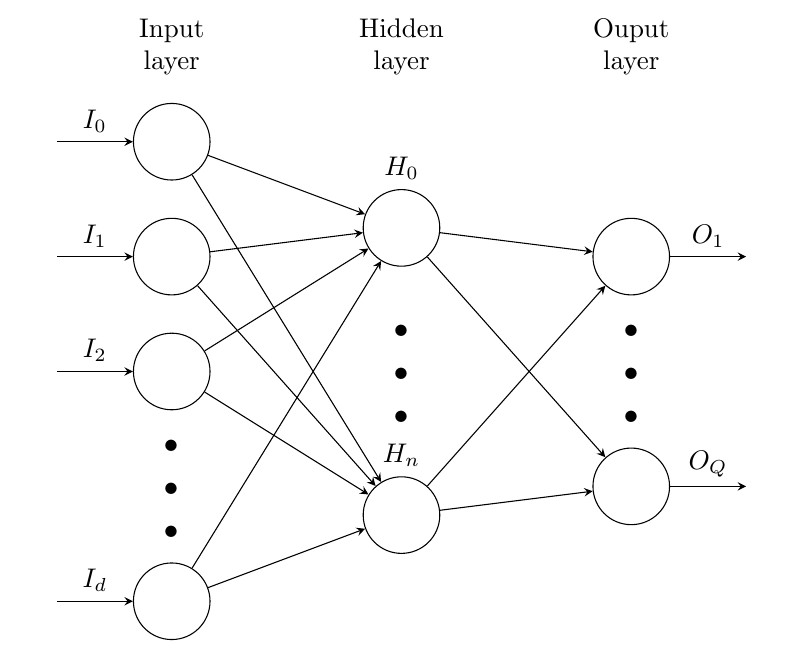
\includegraphics[width=0.8\textwidth]{MultiLabelNet.jpeg}
\caption{\label{fig:MultiLabelNet}Network Topology For Multi-lable classification}
\end{figure}

The network has $d$ input neurons which correspond to a $d$-dimensional feature vector, while last $Q$ neurons represent a combination of output labels. There is a hidden layer in figure \ref{fig:MultiLabelNet} which owns $n$ hidden neurons. The input layer is fully connected with hidden layer and the same connecting method is deployed between hidden layer and the output layer. So there are $d \times n$ weights $(W_{ih}, 1 \leq i \leq d, 1 \leq h \leq n)$ between the input layer and the hidden layer and $n \times q$ weights $(W_{ho}, 1 \leq h \leq n , 1 \leq o \leq q)$ between the hidden layer and the output layer. The bias parameters are represented as $I_{0}$ and  $H_{0}$.

Because the task of multi-label learning is to predict labels of test samples, it needs to evaluate the global error of the model as:
\begin{equation}\label{eq:MultiLableError}
E = \sum_{i=1}^m E_{i}
\end{equation}
$E_{i}$ is the error on sample $x_{i}$ which can be defined as:
\begin{equation}\label{eq:MultiLableSamError}
E_{i} = \sum_{j=1}^Q (c_{j}^i - d_{j}^i)^2
\end{equation}
where $c_{j}^i = c_{j}(x_{i})$ is the predicted $j$-th label by the model on sample $x_{i}$, and $d_{j}^i$ is the actual $j$-th label of sample $x_{i}$. The actual label has value of either $+1 (j \in \mathcal{Y_{i}})$ or $-1 (j \notin \mathcal{Y_{i}})$.

Various learning algorithms can be used to learn a model based on the training dataset. The Backpropagation(BP) algorithm is deployed to learn from errors. However, original BP algorithm could be improper in multi-label learning because the error function \ref{eq:MultiLableSamError} neglects the correlations among labels of a sample. In original BP algorithm, the error function \ref{eq:MultiLableSamError} limits on individual label discrimination, whether a specific label $j \in \mathcal{Y}$ belongs to the sample $x_{i}$ or not. It should take into consideration that labels in $Y_{i}$ are more important than those outside of $Y_{i}$. A new global error function is defined as:
\begin{equation}\label{eq:MultiLableGlobalError}
E = \sum_{i=1}^m E_{i} = \sum_{i=1}^m \frac{1}{|Y_{i}||\hat{Y}_{i}|} \sum_{(k,l) \in Y_{i} \times \hat{Y_{i}}} exp(-(c_{k}^i-c_{l}^i))
\end{equation}
In the error function \ref{eq:MultiLableGlobalError}, the $i$-th errors on the $i$-th sample $(x_{i},Y_{i})$ are accumulated. $\hat{Y}_{i}$ is complementary set of $Y_{i}$ in $\mathcal{Y}$ and $|\cdot|$ computes the cardinality of a set. Specifically, the item, $c_{k}^i-c_{l}^i$, represents the difference between the output labels of the model on a label which belongs to sample $x_{i}$ and a label which does not belong to the same sample. The error function\ref{eq:MultiLableGlobalError} shows that bigger difference leads to better performance. Additionally, the negation of the difference is put into the exponential function to sharply penalize the $i$-th term if $c_{k}^i$ is much smaller than $c_{l}^i$. The sum of $i$-th error term accumulates difference between outputs of any pair of labels which are the one belonging to the sample and the other one not belonging to it. The sum is normalized by the numbers of all pairs, $|Y_{i}||\hat{Y}_{i}|$. And then, the correlations between pair labels are computed. In the other words, labels in $Y_{i}$ should get larger output value than labels in $\hat{Y}_{i}$.

As previous statement, the error function \ref{eq:MultiLableGlobalError} calculates the difference between output labels. The task of learning is minimizing the error function \ref{eq:MultiLableGlobalError} via enlarging output values of labels belonging to the training samples and diminishing the output values of the labels not belonging to it. If the training dataset can cover the distribution of the whole sample space, neural network model can learn it through minimizing error function by feeding training samples.

\subsection{Error Function}

The basic goal of regression problems is to figure out the conditional distribution of the output labels, given the input samples. It is common to use a sum-of-squares error function.

The basic goal of classification problems is to figure out the posterior probabilities of class types, given the input samples. Except for sum-of-squares error function, there are some more approximate error functions which can be considered.

The central goal in training a neural network is to model the hidden generator of the samples instead of memorizing the training samples. Therefore, the best prediction of an input sample can be found if the network can present a new value for the sample. Because the general and complete characterization of the generator of the dataset is the probability density $p(x,t)$. It is available to decompose a joint probability density into the product of the conditional density of the labels, the input data and the density of input data,
\begin{equation}\label{eq:JointProbDensity}
p(x,t) = p(t|x)p(x)
\end{equation}
where $p(t|x)$ represents the probability density of $t$ if $x$ is a distinct label and $p(x)$ represents the density of $x$
\begin{equation}\label{eq:ProbDensityX}
p(x) = \int p(t,x)dt
\end{equation}

Most error functions can be obtained from the idea of maximum likelihood. For training dataset, 
\begin{equation}\label{eq:LikelihoodLoss}
L = \coprod_{\substack{n}}  p(t^n|x^n)p(x^n)
\end{equation}
where each sample is picked out randomly from the same  distribution and their probabilities can be multiplied. The error function can be represented by minimizing the negative logarithm of the likelihood since the negative logarithm is a monotonic function.
\begin{equation}\label{eq:LikelihoodErrorFunc}
E = -ln L = -\sum_{\substack{n}} ln p(t^n|x^n) - \sum_{\substack{n}}lnp(x^n)
\end{equation}
where $E$ is notated as an error function. The task of the neural network is to model the conditional probability density $p(t|x)$. And the second term is independent with the parameters in neural networks.  We can simplify \ref{eq:LikelihoodErrorFunc} to
\begin{equation}\label{eq:SimLikelihoodErrorFunc}
E = -ln L = -\sum_{\substack{n}} ln p(t^n|x^n) + C
\end{equation}
It is worth noting that error functions are dependent on different assumptions of the forms of the conditional distribution $p(t|x)$. In this classification task, $t$ represents labels which act as class members or the prediction of the probabilities of class members.

\subsection{Cross Entropy}

The Mean Square Error is a common risk metric comparable to the predicted value of the squared error loss. It is simple to implementation and non-negative. However, it has the disadvantage of heavily weighting outliers\citep{bermejo2001oriented}.

Given that there are two discrete distributions $p(x)$ and $q(x)$ over the same variable $x$. The relative entropy, relating to cross entropy, is a measurement of the distance between samples:
\begin{equation}\label{eq:RelativeEngtropy}
D_{pq}(p(x), q(x)) = \sum_{\substack{x}}q(x)ln\frac{q(x)}{p(x)}
\end{equation}
where the relative entropy is not a true metric because \ref{eq:RelativeEngtropy} could not be symmetric in the interchange $p \leftrightarrow q$ and probably not satisfy the triangle inequality.

Cross entropy loss, also named logistic regression loss, is an alternative measurement of a probability distribution. The measure is commonly used in neural networks. It can be used to evaluate the posterior probabilities of class membership.

Given that training a neuron, which has several input data, $x_{1}, x_{2},...,$ with weights $w_{1}, w_{2},...,$ and a bias, $b$, the outputs, for example two classes, can be represented as the weighted sum of the input data.
\begin{equation}\label{eq:EquationNN}
a = f(x) = \sum_{i}w_{i}x_{i} + b
\end{equation}
Then the cross entropy cost function is
\begin{equation}\label{eq:TwoClassCrossEntropyCostFunc}
C = -\frac{1}{n} \sum_x \left[y \ln a + (1-y ) \ln (1-a) \right]
\end{equation}
where $n$ is the number of training samples, $a$ is the prediction result and $y$ is actual result.

The cross entropy can act as a cost function because of two properties. First, $C$ is non-negative, because the items of logarithms are in the range $[0,1]$ and there is a minus sign at the beginning of the sum. Second, if the prediction output is close to the actual value for all training samples, the loss value, $C$, will be close to $0$. Given that $y = 0$ and the prediction value $a \approx 0$, the first item in \ref{eq:TwoClassCrossEntropyCostFunc} is $0$ while the second item is $-\ln(1-a) \approx 0$. The similar situation occurs for situation, $y = 1$ and $a \approx 1$. Therefore, the value of cost function will be small, if the prediction value is close to the actual value.

In total, the cross entropy tends to $0$, when the neuron acts better at predicting the output $y$ for total training inputs $x$. The two properties are basic to a cost function. Although the quadratic cost function satisfy the properties, the cross entropy has the advantage on avoiding the issue of learning curve slowing down. To illustrate the advantage, the partial derivative of the cross entropy cost function can be done with the respect to the weights. Applying the chain rule twice on \ref{eq:TwoClassCrossEntropyCostFunc}
\begin{eqnarray}\label{eq:DerCrossEntropyCostFunc}
  \frac{\partial C}{\partial w_j} & = & -\frac{1}{n} \sum_x \left(
    \frac{y }{f(x)} -\frac{(1-y)}{1-f(x)} \right)
  \frac{\partial f}{\partial w_j} \\
 & = & -\frac{1}{n} \sum_x \left( 
    \frac{y}{f(x)}-\frac{(1-y)}{1-f(x)} \right)f'(x) x_j.
\end{eqnarray}
where the second equation can be represented as
\begin{equation}\label{eq:SecondDerCrossEntropyCostFunc}
  \frac{\partial C}{\partial w_j} = \frac{1}{n}  \sum_x \frac{f'(x) x_j}{f(x) (1-f(x))} (f(x)-y)
\end{equation}
Because the defination of the sigmoid function is $f(x) =1/(1+e^{-x})$ and the derivative of sigmoid function is $f'(x) =f(x)(1-f(x))$. Then the items $f'(x)$ and $f(x) =1/(1+e^{-x})$ cancel in the equation and it becomes
\begin{equation}\label{eq:SimDerCrossEntropyCostFunc}
 \frac{\partial C}{\partial w_j} =  \frac{1}{n} \sum_x x_j(f(x)-y)
\end{equation}
The equation shows that the rate of learning weights is controlled by $f(x) - y$. The larger the error is, the faster the neuron learns. In particular, the property avoids the learning slowdown because the derivative item $f'(x)$ gets canceled out in the quadratic cost.

In the similar way, the bias can be computed by the partial derivative.
\begin{equation}\label{eq:BiasCrossEntropyCostFunc}
\frac{\partial C}{\partial b} = \frac{1}{n} \sum_x (f(x)-y)
\end{equation}


\subsection{Training and Testing}

Following the training process, gradient descent is used to minimize the global error function with backpropagation. 

To train a sample $(x_{i}, Y_{i})$, in which $x_{i}$ is the input data and $Y_{i}$ is the associated label, the predicted output labels computed by the neural network for is
\begin{equation}\label{eq:MultiLabelActivation}
c_{k} = f(netc_{k} + \theta_{k})
\end{equation}
where $\theta_{k}$ is the bias units of $k$ layer, $f()$ is the activation function of the output neurons which is a $tanh$ function\ref{eq:tanh} in this project. $netc_{k}$ is the input data of the layer:
\begin{equation}\label{eq:MultiLabel}
netc_{k} = \sum_{s=1}^M b_{s}w_{sk}
\end{equation}
where $w_{sk}$ is the weights for layers $s$ and $k$, while $M$ is the number of neurons in the hidden layer.

As $tanh$ function is differentiable, the general error of the $k$-th output neuron can be defined:
\begin{equation}\label{eq:MultiLableErrorDif}
d_{k} = -\frac{\partial E}{\partial netc_{k}}
\end{equation}
combining with \ref{eq:MultiLabelActivation}, we can get
\begin{equation}\label{eq:MultiLableChainRule}
d_{k} = -\frac{\partial E_{i}}{\partial c_{j}} \frac{\partial c_{j}}{\partial netc_{k}} = - \frac{\partial E_{i}}{\partial c_{j}} f'(netc_{k} + \theta_{k})
\end{equation}
With considering global error function \ref{eq:MultiLableGlobalError}
\begin{equation}\label{eq:MultiLablePartialC}
\frac{\partial E_{i}}{\partial c_{j}}= 
\begin{cases}
    -\frac{1}{|Y_{i}||\hat{Y}_{i}|} \sum_{l \in \hat{Y}_{i}} exp(-(c_{j} - c_{l}))       & \quad \text{if } j \in Y_{i}\\
    \frac{1}{|Y_{i}||\hat{Y}_{i}|} \sum_{k \in Y_{i}} exp(-(c_{k} - c_{j}))       & \quad \text{if } j \in \hat{Y}_{i}\\
  \end{cases}
\end{equation}
with derivation of $tanh$, and substituting it with \ref{eq:MultiLableChainRule} and \ref{eq:MultiLablePartialC} we can get
\begin{equation}\label{eq:MultiLableGenErr}
d_{k}= 
\begin{cases}
    \big(-\frac{1}{|Y_{i}||\hat{Y}_{i}|} \sum_{l \in \hat{Y}_{i}} exp(-(c_{j} - c_{l}))\big)(1+c_{j})(1-c_{j})       & \quad \text{if } j \in Y_{i}\\
    \big(\frac{1}{|Y_{i}||\hat{Y}_{i}|} \sum_{k \in Y_{i}} exp(-(c_{k} - c_{j}))\big)(1+c_{j})(1-c_{j})       & \quad \text{if } j \in \hat{Y}_{i}\\
  \end{cases}
\end{equation}
According to the previous method, we can define the general error of the $s$-th hidden neuron:
\begin{equation}\label{eq:MultiLableGenErrS}
e_{s} = - \frac{\partial E_{i}}{\partial netb_{s}}
\end{equation}
with $b_{s} = f(netb_{s} + \lambda_{s})$ and chain rule,
\begin{equation}\label{eq:MultiLablePartialE}
e_{s} = - \frac{\partial E_{i}}{\partial b_{s}} \frac{\partial b_{s}}{\partial netb_{s}} = - \big( \sum_{j=1}^Q \frac{\partial E_{i}}{\partial netc_{j}} \frac{\partial netc_{j}}{\partial b_{s}}\big)f'(netb_{s} + \lambda_{s})
\end{equation}
For $d_{j} = - \frac{\partial E_{i}}{\partial netc_{j}}$ and $netc_{j} = \sum_{s=1}^M b_{s}w_{sj}$, then 
\begin{equation}\label{eq:MultiLableGenErrEs}
e_{s} = \big( \sum_{j=1}^Q d_{j} \times \frac{\partial (\sum_{s=1}^M b_{s}w_{sj})}{\partial b_{s}}\big) f'(netb_{s} + \lambda_{s}) = \big( \sum_{j=1}^Q d_{j}w_{sj}\big) f'(netb_{s} + \lambda_{s})
\end{equation}
As function $f()$ is $tanh$, we get
\begin{equation}\label{eq:MultiLableGenErrEsFin}
e_{s} = \big( \sum_{j=1}^Q d_{j}w_{sj}\big) (1+b_{s})(1-b_{s})
\end{equation}
The Stochastic Gradient Descent(SGD) is used to approximate function.
\begin{equation}\label{eq:MultiLableUpdateWeights}
\Delta w_{sj} = -\alpha \frac{\partial E_{i}}{\partial w_{sj}} = \alpha \frac{\partial E_{i}}{\partial netc_{j}} \frac{\partial netc_{j}}{\partial w_{sj}} = \alpha d_{j}b_{s}
\end{equation}
\begin{equation}\label{eq:MultiLableUpdateHidWeights}
\Delta v_{hs} = -\alpha \frac{\partial E_{i}}{\partial v_{hs}} = \alpha \frac{\partial E_{i}}{\partial netb_{s}} \frac{\partial netb_{s}}{\partial v_{hs}} = \alpha e_{s}a_{h}
\end{equation}
while the bias are updated according to
\begin{equation}\label{eq:MultiLableUpdateBias}
\Delta \theta_{j} = \alpha d_{j} \text{ } \Delta \lambda_{s} = \alpha e_{s}
\end{equation}
in previous Equations, $\alpha$ is learning rate in the range of $[0.0 \text{ } 1.0]$.

In the training process, a learning algorithm has been set up with backpropagation. Moreover, training samples are fed into the neural network in each epoch. After all training samples $(x, Y)$ fed into network, weights and bias are updated through equations\ref{eq:MultiLableUpdateWeights} and \ref{eq:MultiLableUpdateBias}. The training samples are fed into the network iteratively while global error value decreases. Finally, the error value converges to a minimum value.

In the testing process, the network predicts a sample which has a set of actual labels $c_{j} (j = 1,2,...,Q)$ by ranking the labels. Because the output value of each label is in range $[-1.0,1.0]$, a threshold function $t(x)$ is used to determine associated label set for the sample $x$. A large margin ranking system\citep{elisseeff2001kernel} is adopted to generalize the sets. $t(x)$ is a linear function, $t(x) = w^T\cdot c(x) + b$, where $c(x) = (c_{1}(x), c_{2}(x),...,c_{Q}(x))$ is a $Q$-dimensional vector which represents $j$ output labels of a sample. Learning the threshold function $t(x)$ follows the steps. For every training sample $(x_{i}, Y_{i}) (1 \leq i \leq m)$, the relation between $c(x_{i})$ and target value $t(x_{i})$ is:
\begin{equation}\label{eq:MultiLableThreshFunc}
t(x_{i}) =  \operatorname{arg\,max}_t (|\{k|k \in Y_{i}, c_{k}^i \leq t\}| + |\{l|l \in \hat{Y}_{i}, c_{l}^i \geq t\}|) 
\end{equation}
If there are several minimum values and optimal values are in a division, the middle value of the division is chosen. The task of learning the parameters of threshold function is to solve the matrix equation $\Phi \cdot w' = t$. The matrix $\Phi$ has dimensions $m \times (Q + 1)$ in which $i$-th vector is $(c_{1}^i, c_{2}^2,...,c_{Q}^i,1)$, $w'$ is $(Q+1)$ dimensional vector $(w,b)$ and $t$ is the $m$ dimensional vector $(t(x_{1}), t(x_{2}),...,t(x_{m}))$. Linear least squares is used to find the solution of the equation. Given a sample $x$, the network predicts output label vector $c(x)$ and the threshold value for $x$ is gotten by solving equation$t(x) = w^T \cdot c(x) + b$.

The computational complexity of evaluating derivatives of the error function is linear with the neuron numbers. Three main components are composed of computation, feedforward process, backpropagation process and updating weights process. In the feed-forward process, to compute $b_{i}$ and $c_{j}$, the computation cost is mainly on evaluating the sums and activation function. In the backpropagation process(\ref{eq:MultiLableGenErr}and\ref{eq:MultiLableGenErrEsFin}), the computational complexity of $d_{k}$ and $e_{s}$ is $O(Q)$. In the updating weights process, the overall computational cost is $O(W)$ where $W$ is the total number of weights . 





















 % Conclusion

%% ----------------------------------------------------------------
% Now begin the Appendices, including them as separate files

\addtocontents{toc}{\vspace{2em}} % Add a gap in the Contents, for aesthetics

\appendix % Cue to tell LaTeX that the following 'chapters' are Appendices

% Appendix A

\chapter{Appendix Title Here}
\label{AppendixA}
\lhead{Appendix A. \emph{Appendix Title Here}}

Write your Appendix content here.	% Appendix Title

%\input{./Appendices/AppendixB} % Appendix Title

%\input{./Appendices/AppendixC} % Appendix Title

\addtocontents{toc}{\vspace{2em}}  % Add a gap in the Contents, for aesthetics
\backmatter

%% ----------------------------------------------------------------
\label{Bibliography}
\lhead{\emph{Bibliography}}  % Change the left side page header to "Bibliography"
\bibliographystyle{unsrtnat}  % Use the "unsrtnat" BibTeX style for formatting the Bibliography
\bibliography{Bibliography}  % The references (bibliography) information are stored in the file named "Bibliography.bib"

\end{document}  % The End
%% ----------------------------------------------------------------